% Options for packages loaded elsewhere
\PassOptionsToPackage{unicode}{hyperref}
\PassOptionsToPackage{hyphens}{url}
%
\documentclass[
  12pt,
  oneside]{book}
\usepackage{amsmath,amssymb}
\usepackage{setspace}
\usepackage{iftex}
\ifPDFTeX
  \usepackage[T1]{fontenc}
  \usepackage[utf8]{inputenc}
  \usepackage{textcomp} % provide euro and other symbols
\else % if luatex or xetex
  \usepackage{unicode-math} % this also loads fontspec
  \defaultfontfeatures{Scale=MatchLowercase}
  \defaultfontfeatures[\rmfamily]{Ligatures=TeX,Scale=1}
\fi
\usepackage{lmodern}
\ifPDFTeX\else
  % xetex/luatex font selection
\fi
% Use upquote if available, for straight quotes in verbatim environments
\IfFileExists{upquote.sty}{\usepackage{upquote}}{}
\IfFileExists{microtype.sty}{% use microtype if available
  \usepackage[]{microtype}
  \UseMicrotypeSet[protrusion]{basicmath} % disable protrusion for tt fonts
}{}
\makeatletter
\@ifundefined{KOMAClassName}{% if non-KOMA class
  \IfFileExists{parskip.sty}{%
    \usepackage{parskip}
  }{% else
    \setlength{\parindent}{0pt}
    \setlength{\parskip}{6pt plus 2pt minus 1pt}}
}{% if KOMA class
  \KOMAoptions{parskip=half}}
\makeatother
\usepackage{xcolor}
\usepackage[left=4cm, right=3cm, top=2.5cm, bottom=2.5cm]{geometry}
\usepackage{color}
\usepackage{fancyvrb}
\newcommand{\VerbBar}{|}
\newcommand{\VERB}{\Verb[commandchars=\\\{\}]}
\DefineVerbatimEnvironment{Highlighting}{Verbatim}{commandchars=\\\{\}}
% Add ',fontsize=\small' for more characters per line
\usepackage{framed}
\definecolor{shadecolor}{RGB}{248,248,248}
\newenvironment{Shaded}{\begin{snugshade}}{\end{snugshade}}
\newcommand{\AlertTok}[1]{\textcolor[rgb]{0.94,0.16,0.16}{#1}}
\newcommand{\AnnotationTok}[1]{\textcolor[rgb]{0.56,0.35,0.01}{\textbf{\textit{#1}}}}
\newcommand{\AttributeTok}[1]{\textcolor[rgb]{0.13,0.29,0.53}{#1}}
\newcommand{\BaseNTok}[1]{\textcolor[rgb]{0.00,0.00,0.81}{#1}}
\newcommand{\BuiltInTok}[1]{#1}
\newcommand{\CharTok}[1]{\textcolor[rgb]{0.31,0.60,0.02}{#1}}
\newcommand{\CommentTok}[1]{\textcolor[rgb]{0.56,0.35,0.01}{\textit{#1}}}
\newcommand{\CommentVarTok}[1]{\textcolor[rgb]{0.56,0.35,0.01}{\textbf{\textit{#1}}}}
\newcommand{\ConstantTok}[1]{\textcolor[rgb]{0.56,0.35,0.01}{#1}}
\newcommand{\ControlFlowTok}[1]{\textcolor[rgb]{0.13,0.29,0.53}{\textbf{#1}}}
\newcommand{\DataTypeTok}[1]{\textcolor[rgb]{0.13,0.29,0.53}{#1}}
\newcommand{\DecValTok}[1]{\textcolor[rgb]{0.00,0.00,0.81}{#1}}
\newcommand{\DocumentationTok}[1]{\textcolor[rgb]{0.56,0.35,0.01}{\textbf{\textit{#1}}}}
\newcommand{\ErrorTok}[1]{\textcolor[rgb]{0.64,0.00,0.00}{\textbf{#1}}}
\newcommand{\ExtensionTok}[1]{#1}
\newcommand{\FloatTok}[1]{\textcolor[rgb]{0.00,0.00,0.81}{#1}}
\newcommand{\FunctionTok}[1]{\textcolor[rgb]{0.13,0.29,0.53}{\textbf{#1}}}
\newcommand{\ImportTok}[1]{#1}
\newcommand{\InformationTok}[1]{\textcolor[rgb]{0.56,0.35,0.01}{\textbf{\textit{#1}}}}
\newcommand{\KeywordTok}[1]{\textcolor[rgb]{0.13,0.29,0.53}{\textbf{#1}}}
\newcommand{\NormalTok}[1]{#1}
\newcommand{\OperatorTok}[1]{\textcolor[rgb]{0.81,0.36,0.00}{\textbf{#1}}}
\newcommand{\OtherTok}[1]{\textcolor[rgb]{0.56,0.35,0.01}{#1}}
\newcommand{\PreprocessorTok}[1]{\textcolor[rgb]{0.56,0.35,0.01}{\textit{#1}}}
\newcommand{\RegionMarkerTok}[1]{#1}
\newcommand{\SpecialCharTok}[1]{\textcolor[rgb]{0.81,0.36,0.00}{\textbf{#1}}}
\newcommand{\SpecialStringTok}[1]{\textcolor[rgb]{0.31,0.60,0.02}{#1}}
\newcommand{\StringTok}[1]{\textcolor[rgb]{0.31,0.60,0.02}{#1}}
\newcommand{\VariableTok}[1]{\textcolor[rgb]{0.00,0.00,0.00}{#1}}
\newcommand{\VerbatimStringTok}[1]{\textcolor[rgb]{0.31,0.60,0.02}{#1}}
\newcommand{\WarningTok}[1]{\textcolor[rgb]{0.56,0.35,0.01}{\textbf{\textit{#1}}}}
\usepackage{longtable,booktabs,array}
\usepackage{calc} % for calculating minipage widths
% Correct order of tables after \paragraph or \subparagraph
\usepackage{etoolbox}
\makeatletter
\patchcmd\longtable{\par}{\if@noskipsec\mbox{}\fi\par}{}{}
\makeatother
% Allow footnotes in longtable head/foot
\IfFileExists{footnotehyper.sty}{\usepackage{footnotehyper}}{\usepackage{footnote}}
\makesavenoteenv{longtable}
\usepackage{graphicx}
\makeatletter
\newsavebox\pandoc@box
\newcommand*\pandocbounded[1]{% scales image to fit in text height/width
  \sbox\pandoc@box{#1}%
  \Gscale@div\@tempa{\textheight}{\dimexpr\ht\pandoc@box+\dp\pandoc@box\relax}%
  \Gscale@div\@tempb{\linewidth}{\wd\pandoc@box}%
  \ifdim\@tempb\p@<\@tempa\p@\let\@tempa\@tempb\fi% select the smaller of both
  \ifdim\@tempa\p@<\p@\scalebox{\@tempa}{\usebox\pandoc@box}%
  \else\usebox{\pandoc@box}%
  \fi%
}
% Set default figure placement to htbp
\def\fps@figure{htbp}
\makeatother
\setlength{\emergencystretch}{3em} % prevent overfull lines
\providecommand{\tightlist}{%
  \setlength{\itemsep}{0pt}\setlength{\parskip}{0pt}}
\setcounter{secnumdepth}{5}
% ---------- Hyphenation / Layout ----------
\usepackage[none]{hyphenat}   % Disable automatic hyphenation
\raggedbottom                 % Avoid large vertical stretches caused by floats

% ---------- TOC / Front matter ----------
\usepackage[nottoc,notlot,notlof]{tocbibind}  % Add bibliography to TOC, but not toc/lot/lof entries themselves
\usepackage{pdfpages}                         % Insert external PDF pages (e.g., cover, declaration)

% ---------- Captions / Subfigures ----------
\usepackage[width=\textwidth]{caption}  % Ensure captions fit within text width
\usepackage{subfig}                     % Provides \subfloat, compatible with bookdown fig.subcap

% ---------- Floats ----------
\usepackage{float}     % Provides [H] option for placing floats exactly here
\usepackage{placeins}  % Provides \FloatBarrier to clear pending floats

% ---------- Clear floats before new sections ----------
\usepackage{etoolbox}
\makeatletter
\@ifundefined{chapter}{}{\pretocmd{\chapter}{\FloatBarrier}{}{}}
\@ifundefined{section}{}{\pretocmd{\section}{\FloatBarrier}{}{}}
\@ifundefined{subsection}{}{\pretocmd{\subsection}{\FloatBarrier}{}{}}
\makeatother

% =========================================================
%                  Header / Footer (oneside)
% =========================================================
% =========================================================
%                  Header / Footer (oneside)
% =========================================================
\usepackage{fancyhdr}

% Ensure enough space for headers
\setlength{\headheight}{15pt}

% Default page style
\pagestyle{fancy}
\fancyhf{}                                 % Clear all header/footer fields
\fancyhead[R]{\nouppercase{\leftmark}}     % Right header = current chapter
\fancyfoot[C]{\thepage}                    % Footer center = page number
\renewcommand{\headrulewidth}{0pt}         % No header line
\renewcommand{\footrulewidth}{0pt}         % No footer line

% --- Ensure \leftmark updates correctly ---
% Define what goes into \leftmark when a new chapter starts
\renewcommand{\chaptermark}[1]{%
  \markboth{\chaptername\ \thechapter.\ #1}{}%
}

% Apply the same style to "plain" pages (chapter openings, float pages)
\fancypagestyle{plain}{%
  \fancyhf{}
  \fancyhead[R]{\nouppercase{\leftmark}}
  \fancyfoot[C]{\thepage}
  \renewcommand{\headrulewidth}{0pt}
  \renewcommand{\footrulewidth}{0pt}
}

% --- Fix for delayed header update ---
% Force headers to refresh immediately at the start of every chapter
\usepackage{etoolbox}
\makeatletter
\pretocmd{\chapter}{\thispagestyle{fancy}}{}{}
\makeatother

% =========================================================

\usepackage{afterpage}
\makeatletter
\let\old@chapter\@chapter
\def\@chapter[#1]#2{%
  \old@chapter[#1]{#2}%
  \afterpage{\markboth{\chaptername\ \thechapter.\ #1}{}}%
}
\makeatother
\usepackage{booktabs}
\usepackage{longtable}
\usepackage{array}
\usepackage{multirow}
\usepackage{wrapfig}
\usepackage{float}
\usepackage{colortbl}
\usepackage{pdflscape}
\usepackage{tabu}
\usepackage{threeparttable}
\usepackage{threeparttablex}
\usepackage[normalem]{ulem}
\usepackage{makecell}
\usepackage{xcolor}
\usepackage[style=apa,]{biblatex}
\addbibresource{book.bib}
\addbibresource{packages.bib}
\addbibresource{test.bib}
\addbibresource{thesisclean.bib}
\usepackage{bookmark}
\IfFileExists{xurl.sty}{\usepackage{xurl}}{} % add URL line breaks if available
\urlstyle{same}
\hypersetup{
  pdftitle={Digital Planning Support in a Data-scarce Context by Estimating Urban Activities : A Case Study in Jaipur City, India},
  hidelinks,
  pdfcreator={LaTeX via pandoc}}

\title{Digital Planning Support in a Data-scarce Context by Estimating Urban Activities : A Case Study in Jaipur City, India}
\author{Miaoyi Li\\
\strut \\
CASA0010, MSc Urban Spatial Science Dissertation\\
\strut \\
Supervisor: Dr Jens Kandt\\
\strut \\
Repository: \url{https://github.com/Aprilmiaoyilee/CASA-Jaipur/}\\
\strut \\
This dissertation is submitted in part requirement for the\\
MSc in the Centre for Advanced Spatial Analysis,\\
Bartlett Faculty of the Built Environment, UCL\\
\strut \\
Word count: 11182}
\date{2025-08-22}

\begin{document}
\maketitle

\setstretch{1.5}
\pagenumbering{roman}

\chapter*{Abstract}\label{abstract}

The lack of timely and disaggregated demographic and economic information often constrains urban digital planning in data-scarce contexts. This study examines the application of open and remote sensing data in generating alternative evidence for planning, using Jaipur, India, as a case study. Two complementary strands of analysis were developed: grid-level population estimation through Multiscale Geographically Weighted Regression (MGWR), and the construction of an Economic Activity Index (EAI) to capture spatial economic variation via principal component analysis (PCA) of indicators including built-up area, points of interest, and nighttime lights.

The results show that while the population model broadly reproduced settlement structures, it also revealed systematic biases. Meanwhile, the EAI provided a composite representation of urban economic intensity. Both outputs were delivered through a Google Earth Engine (GEE) web application, enabling planners to interact with estimates and underlying variables.

By demonstrating how open data and cloud-based tools can generate and share population and economic activity estimates, this study presents a practical and replicable pathway for expanding digital planning support in contexts where conventional statistics are limited.

\pagenumbering{roman}

\chapter*{Declaration}\label{declaration}

I, Miaoyi Li, hereby declare that the work presented in this dissertation is entirely my own original work, and that all sources have been properly acknowledged. Furthermore, I declare that I used Google AI Studio - Gemini 2.5 to assist in summarizing research notes, code debugging and final proofreading.

\chapter*{Acknowledgements}\label{acknowledgements}

I would like to express my sincere gratitude to my supervisor, Dr.~Jens Kandt, for his endless patience and invaluable advice throughout my study. Jens's encouragement and prompt feedback during our discussions and email exchanges greatly motivated me and helped shape this work.

I am also deeply grateful to our colleagues from the Jaipur project, especially Dr.~Nand Kumar and Prof.~Mahesh Jat from Malaviya National Institute of Technology (MNIT) Jaipur, for their assistance with data access and their insightful suggestions on refining my methodologies. I would also like to thank all others involved in the project, which gave me a concrete understanding of the research process in practical planning --- from data cleaning to analysis and visualisation --- in a Global South context.

Most importantly, my heartfelt thanks go to my family and friends for their unwavering support throughout my whole learning journey in London.

% Trigger ToC creation in LaTeX
\setcounter{tocdepth}{3}
\tableofcontents
\listoffigures
\listoftables

\chapter*{Abbreviations}\label{abbreviations}

\begin{longtable}{ll}
\toprule
\textbf{Term} & \textbf{Abbreviation}\\
\midrule
Akaike Information Criterion, corrected & AICc\\
Economic Activity Index & EAI\\
First/Second Principal Component & PC1/PC2\\
Geographical Random Forest & GRF\\
Global Human Settlement Layer & GHSL\\
\addlinespace
Google Earth Engine & GEE\\
Gross Domestic Product & GDP\\
Information and Communication Technologies & ICT\\
Jaipur Development Authority & JDA\\
Jaipur Municipal Corporation & JMC\\
\addlinespace
Land Use and Land Cover & LULC\\
Light Detection and Ranging & LiDAR\\
Moderate Resolution Imaging Spectroradiometer & MODIS\\
Multiscale Geographically Weighted Regression & MGWR\\
Nighttime Light(s) & NTL\\
\addlinespace
Normalized Difference Vegetation Index & NDVI\\
OpenStreetMap & OSM\\
Participatory Geographic Information System & PGIS\\
Planning Support Systems & PSS\\
Points of Interest & POI\\
\addlinespace
Principal Component Analysis & PCA\\
Rajasthan State Industrial Development and Investment Corporation & RIICO\\
Random Forest & RF\\
Synthetic Aperture Radar & SAR\\
Visible Infrared Imaging Radiometer Suite & VIIRS\\
\addlinespace
Volunteered Geographic Information & VGI\\
\bottomrule
\end{longtable}

\chapter{Introduction}\label{introduction}

\pagenumbering{arabic} 

Urban planning in data-scarce contexts poses persistent challenges, particularly in rapidly growing cities of the Global South. Reliable demographic and economic data are often unavailable, outdated, or too aggregated to guide decisions effectively. This constrains planners' ability to design inclusive and sustainable strategies, while the reliance on costly surveys or proprietary datasets delays decision-making and excludes many stakeholders from the planning process. In India, these difficulties are especially pronounced: fast-paced urbanisation has created mounting demands for housing, infrastructure, and services, yet planning institutions frequently lack the disaggregated evidence needed to address inequality and manage growth effectively. These conditions underline the urgency of developing alternative pathways to support planning through open and digital tools.

One promising direction is the use of remote sensing and open data. Datasets such as building footprints, points of interest (POI), road networks, and nighttime lights (NTL) are increasingly available at high resolution and consistent across cities. While such proxies cannot fully substitute conventional surveys, they provide valuable insights into settlement patterns and urban activities. At the same time, advances in spatial modelling and cloud-based platforms now enable these outputs to be delivered in interactive and transparent forms. Together, these developments open new opportunities to strengthen digital planning support in data-scarce contexts.

Jaipur, India, serves as the case study for this work. The city exemplifies both the promise and difficulty of planning in a data-scarce environment: it is expanding rapidly, faces pressures of infrastructure provision and inequality, yet lacks up-to-date and disaggregated demographic and economic data. By testing the feasibility of grid-level population estimation and constructing a composite index of economic activity from open data, Jaipur provides an ideal setting to demonstrate how digital planning support can be advanced where conventional evidence is sparse.

Against this backdrop, the central question of this study is: \textbf{How can digital, open-access planning be supported in data-scarce contexts?} To address this, two research questions are posed:

\begin{enumerate}
\def\labelenumi{\arabic{enumi}.}
\tightlist
\item
  \textbf{How can remote sensing and open data be used to estimate urban activity?}
  This question is addressed in two strands:

  \begin{itemize}
  \tightlist
  \item
    \emph{Population estimation}: using ward-level population counts as a baseline, a multiscale geographically weighted regression (MGWR) model is applied to generate grid-level population surfaces, capturing intra-urban variations that ward aggregates cannot reveal.
  \item
    \emph{Economic Activity Index (EAI)}: a composite measure of urban economic vitality is constructed through principal component analysis (PCA), integrating indicators such as road density, POI density and NTL.
  \end{itemize}
\item
  \textbf{How can these analytical results be transformed into forms that support collaborative planning?}
  This question concerns the design of a web-based tool for exploration and use by planners and communities.

  \begin{itemize}
  \tightlist
  \item
    A Google Earth Engine (GEE) app was developed to allow interactive querying of population estimates, including polygon-based selection.
  \item
    The app also aggregates the EAI by ward, enabling users to compare relative economic activity across the city and to examine the contribution of underlying variables.
  \end{itemize}
\end{enumerate}

By tackling these questions, the study contributes to ongoing debates on urban data innovation in the Global South. It demonstrates how grid-level population estimates and composite indices of economic activity can be derived from remote sensing and open data, providing planners with alternative perspectives when up-to-date data is absent. Equally, by delivering outputs through an open-access web platform, it illustrates how digital tools can enhance transparency, accessibility, and collaboration in planning processes. While not substitutes for detailed surveys, these approaches can generate indicative surfaces that inform dialogue, experiments, and decision-making in resource-constrained environments.

The remainder of this thesis is structured as follows. Chapter 2 reviews literature on urban planning in data-scarce contexts, methods for population estimation and economic activity proxies, and the use of digital platforms for planning support. Chapter 3 then introduces the datasets and methods applied in this study, including grid-level population estimation, construction of the EAI, and implementation of a web application. Chapter 4 presents the results for Jaipur, highlighting both expected patterns and local discrepancies. Chapter 5 discusses the implications of these findings for planning support, as well as the limitations and potential directions for future research. Chapter 6 concludes by summarising the main contributions of this study.

\chapter{Literature Review}\label{LR}

Jaipur's participation in India's Smart Cities Mission reflects its ambition to use data-driven approaches for urban governance, but this goal is hindered by scarce, outdated, and low-granularity spatial data---a challenge common across the Global South that constrains evidence-based digital planning, particularly for understanding population distribution and economic vitality. To address these gaps, researchers increasingly turn to remote sensing and open data as alternative evidence sources, while digital urban planning platforms provide a complementary means to integrate and apply such information. However, the effectiveness of these platforms depends heavily on the quality of the underlying data. This chapter reviews literature on digital platforms in the smart city context (Section 2.1), the nature and impacts of urban data scarcity (Section 2.2), Jaipur's specific urban and policy setting (Section 2.3), and alternative datasets and modelling approaches for estimating urban activities (Sections 2.4--2.5), with Section 2.6 summarising these findings to justify the methodological choices adopted in this study.

\section{Digital Urban Planning Platforms in the Era of Smart Cities}\label{digital-urban-planning-platforms-in-the-era-of-smart-cities}

Digital urban planning platforms are central tools in the smart city framework, where Information and Communication Technologies (ICT) are used to improve city management and public services \autocite{przybyszIntegratingCityMaster2024}. These platforms are not merely digital maps, but integrated systems that combine several key functions. First, they integrate data from multiple sources and formats, including geospatial datasets, statistical records, and real-time sensor feeds \autocite{anttiroikoDigitalUrbanPlanning2021}. Second, they provide analysis and visualisation capabilities, such as spatial modelling, pattern recognition, and interactive dashboards, which transform complex data into clear and actionable insights \autocite{repetteEvolutionCityasaPlatformSmart2021}. Third, they offer collaborative and decision-support features, providing planners, policymakers, and citizens with a shared workspace to test scenarios, assess impacts, and co-develop solutions \autocite{anttiroikoDigitalUrbanPlanning2021}. In this way, digital planning platforms convert raw data into usable knowledge that can reshape traditional planning workflows.

In addition to their technical functions, these platforms are changing urban governance and public participation practices. The rise of open government data has made them important channels for publishing and using spatial information, thereby increasing transparency in planning processes \autocite{parasaEmbedOpenData2021}. They also enable new forms of citizen engagement, such as Participatory Geographic Information System (PGIS), Volunteered Geographic Information (VGI), and online co-creation platforms, which allow residents to contribute local knowledge and feedback more easily \autocite{ddambaDataParticipationParticipation2015,haslerDigitalToolsMeans2017}. In India, recent policies have emphasised the value of open geospatial data, encouraging its integration into master plans and other urban development initiatives \autocite{parasaEmbedOpenData2021}. These developments show that digital planning platforms can help make urban governance more inclusive, collaborative, and responsive to local needs.

One of the most common ways to deliver such platforms is through interactive web applications. Web-based GIS platforms allow users to explore and analyse spatial data directly in a browser, removing the need for specialised desktop software and lowering barriers for participation \autocite{gebetsroither-geringerINTERACTIVESPATIALWEBAPPLICATIONS2018}. Cloud-based geospatial platforms such as Google Earth Engine (GEE) further expand these possibilities by combining access to petabyte-scale satellite data with high-performance processing tools \autocite{stamouSatelliteImageryComprehensive2025}. GEE applications have been applied in a wide range of urban studies, including mapping urban extent and estimating urban growth \autocite{wangGoogleEarthEngine2021}, assessing accessibility and characterising urban ecosystems \autocite{carvalhoDelimitationUrbanAreas2018}, and monitoring urban heat island intensity using MODIS and Landsat data to support sustainable development strategies \autocite{galodhaLANDSURFACETEMPERATURE2021}. By embedding such analyses into shareable web maps and dashboards, researchers can make up-to-date spatial insights accessible to policymakers and the public. This demonstrates a practical pathway for implementing digital urban planning platforms and connects directly to the methods used later in this study.

Yet the practical value of these platforms ultimately rests on the evidence they can mobilise. In many Global South cities, including Jaipur, the binding constraint is not the platform itself but the availability, granularity, and openness of the underlying data. The next section (2.2) examines this constraint.

\section{Urban Data Scarcity: Challenges from the Global South}\label{urban-data-scarcity-challenges-from-the-global-south}

In many cities across the Global South, key urban datasets required for effective planning are scarce or inaccessible. Here, urban data scarcity refers to gaps in availability, spatial resolution, timeliness, and interoperability that hinder neighbourhood-scale analysis and cross-sector integration. First, high-granularity population and economic activity data are often lacking: census datasets are typically decennial and aggregated to large spatial units (e.g., wards), which makes them unsuitable for neighbourhood-level analysis \autocite{georganosCensusHeavenUnraveling2022,satterthwaite5UrbanMyths2010}. Second, dynamic behavioural data are costly and challenging to collect through conventional surveys (e.g., origin--destination flows, daily mobility patterns, and consumption behaviours). Third, the informal sector---both in employment and in housing---is often invisible in official statistics despite its significant role in urban economies \autocite{brahmbhattUrbanSlumsDatafying2019}. Finally, institutional ``data silos'' mean that even when datasets exist, they are stored in separate departmental systems without effective sharing mechanisms \autocite{gosling-goldsmithAerialterrestrialDataFusion2025}. This separation restricts the integration needed for digital planning platforms to represent the full picture of the city, including residents' movements, interactions, and economic behaviours.

The impacts of such data scarcity are wide-ranging. Without reliable datasets, evidence-based decision-making is weakened, and planning often relies more on intuition or political negotiation than on rigorous analysis \autocite{duhrSpatialDataRequirements2021}. In land-use and transport planning, this can lead to resource misallocation, such as poorly located infrastructure, underused public facilities or transport routes that do not match actual demand \autocite{shehuChallengesApplyingBig2024}. In public service provision, a lack of granular demographic and socioeconomic data can cause uneven access to education, healthcare and basic utilities, which deepens existing inequalities \autocite{srivastavaSegregatedDataUrban2017}. Public participation is also undermined because, without credible and shared datasets, consultations often turn into unproductive debates driven more by perceptions than by evidence \autocite{delphinObstaclesDevelopmentIntegrated2022}. These issues have been observed in contexts where incomplete datasets have contributed to inefficient infrastructure projects and missed opportunities to integrate blue--green infrastructure into urban plans \autocite{adeloyeKeyChallengesEvidencebased2015,sorensenDataManagementFramework2021}. In practice, the absence of robust and up-to-date evidence chains compromises the ability to design, implement and monitor the interventions that smart city platforms are meant to enable.

These technical and organisational barriers, which lead to data scarcity, often stem from deeper governance and institutional issues. In many contexts, data are treated as strategic assets rather than public goods, and agencies are reluctant to share information across departmental boundaries \autocite{yuKeyChallengesPotential2024}. The lack of clear data standards, privacy regulations and accountability mechanisms further reinforces data fragmentation \autocite{kvalvikTechnologySmartCities2022}. Experiences from smart city initiatives in the Global South show that technological tools cannot succeed without governance systems that encourage transparency, collaboration and citizen engagement \autocite{meijerGoverningSmartCity2016,senguptaSDG11SmartCities2022}. Research on data justice also indicates that new digital datasets can unintentionally increase inequalities if the benefits mainly flow to already advantaged groups \autocite{heeksDataficationDevelopmentMarginalised2019,brahmbhattUrbanSlumsDatafying2019}. These structural barriers, which involve political, social and institutional factors, are as evident in India as in other developing countries. In Jaipur, the combination of limited high-granularity datasets and top-down governance creates specific constraints for digital planning (Section 2.3).

\section{Urban Development and Digital Policy in India and Jaipur}\label{urban-development-and-digital-policy-in-india-and-jaipur}

\subsection{National Context: India's Urbanisation and Digital Agenda}\label{national-context-indias-urbanisation-and-digital-agenda}

India is urbanising at an unprecedented pace. In 2011, the national urban population was around 377 million, and it is projected to exceed 600 million by 2036 \autocite{GearingIndiasRapid2024}. This rapid growth puts intense pressure on infrastructure, public services, and governance systems. Indian cities face long-standing governance issues, such as overlapping responsibilities among agencies, limited fiscal autonomy, and slow implementation of master plans \autocite{ghoshUrbanChallengesIndia2014,singhCitizensParticipationUrban2013}. To respond, the central government has launched major programmes that link urban development with digital transformation. The Smart Cities Mission (SCM), initiated in 2015, aims to improve quality of life through technology-driven solutions, competitive funding, and area-based development \autocite{theministryofhousingandurbanaffairsmohuaSmartCitiesSmartcities2015}. The Digital India initiative launched in 2015 works in parallel to expand broadband connectivity, promote e-governance, and improve public access to information \autocite{ministryofelectronics&itUsDigitalIndia2015}. Together, these programmes create a strong top-down push for Indian cities, including Jaipur, to adopt data-driven planning and management systems.

\subsection{City Context: Jaipur's Urban Structure and Spatial Heterogeneity}\label{city-context-jaipurs-urban-structure-and-spatial-heterogeneity}

Jaipur is the capital of Rajasthan and a major economic, administrative, and cultural hub in north-west India. Its economy combines tourism, manufacturing, handicrafts, and service industries, yet the growing presence of marginal workers and casual labourers underscores the informal sector's increasing importance. The city's spatial form reflects a mix of planned and organic growth. The historic walled city, founded in 1727 according to Vastu Shastra principles, has a compact grid layout and heritage architecture \autocite{jawaidExploringImageabilityWalled2014}. Post-independence expansion led to suburban growth, particularly to the south and west, often in planned layouts (Figure \ref{fig:02LR-land-use}). More recently, growth has concentrated along transport corridors and in peripheral clusters, sometimes developed without comprehensive planning \autocite{jawaidCityProfileJaipur2017}. Administratively, the city is divided into Jaipur Municipal Corporation (JMC) Heritage and JMC Greater, which reinforces spatial and governance heterogeneity. Between 1991 and 2021, the built-up area expanded by over 150\%, while vegetation and vacant land declined sharply (Figure \ref{fig:02LR-built-up}). This uneven growth has created contrasts between dense central wards and sprawling, less-serviced peripheries, leading to differences in infrastructure access, green space provision, and service delivery \autocite{un-habitatCityProfileDiagnostic2021}

\begin{figure}

{\centering 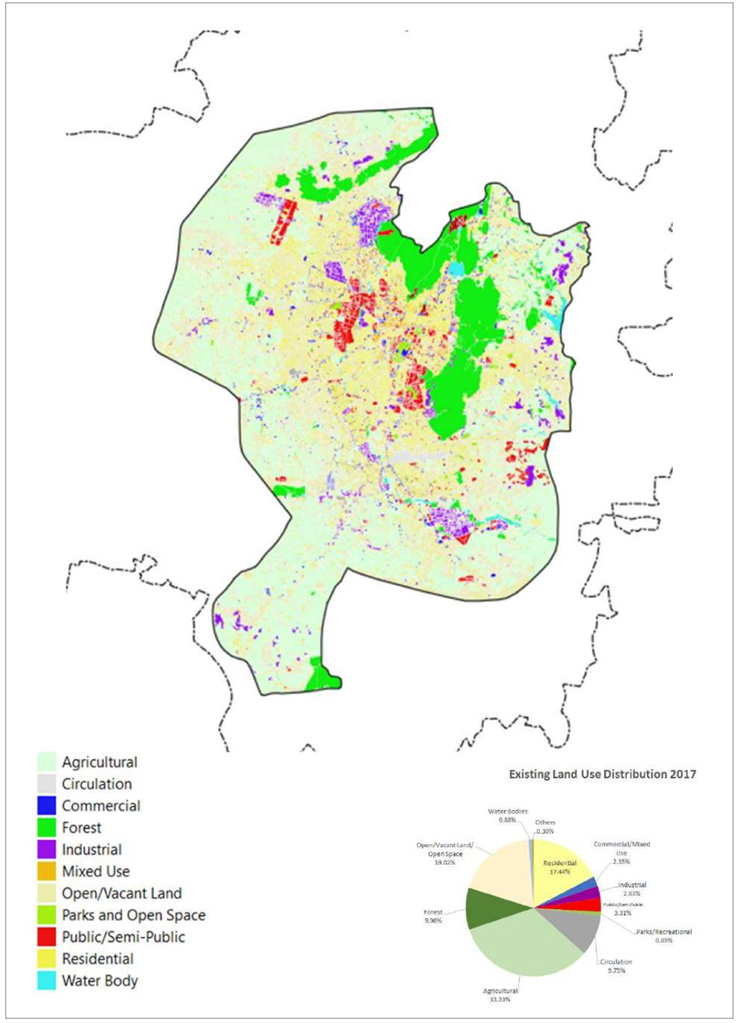
\includegraphics[width=0.6\linewidth]{thesis_images/02LR_land_use} 

}

\caption{Existing Land Use Map of Jaipur Urbanizable Area 2017. Source: Jaipur Master Development Plan 2025.}\label{fig:02LR-land-use}
\end{figure}

\begin{figure}

{\centering 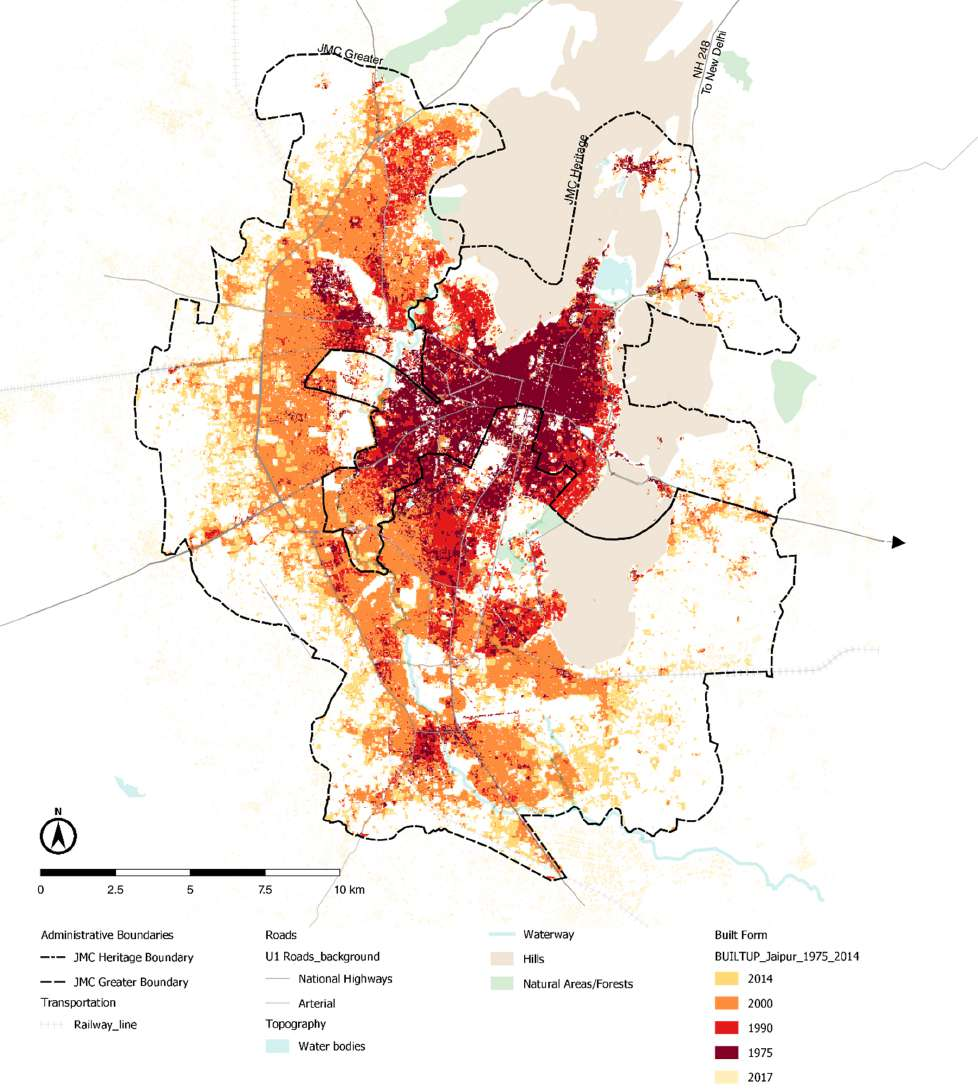
\includegraphics[width=0.6\linewidth]{thesis_images/02LR_built_up} 

}

\caption{ Multi-temporal Classification of JMC Built-up Presence. Source: UN-Habitat.}\label{fig:02LR-built-up}
\end{figure}

\subsection{Local Reality: Digital Initiatives and Data Limitations}\label{local-reality-digital-initiatives-and-data-limitations}

Under the Smart Cities Mission, Jaipur Smart City Limited (JSCL) has implemented both area-based and pan-city projects. In the walled city, projects focus on heritage revitalisation and improved pedestrian and cycling infrastructure. City-wide initiatives include a public bicycle sharing system, environmental monitoring sensors, solid waste management improvements, and the development of a central command-and-control centre for transport and traffic management \autocite{jaipursmartcitylimitedJaipurSmartCity2025}. These efforts signal an ambition to embed digital tools into urban management. However, the underlying data infrastructure remains weak. There is no dedicated local open data portal; most publicly available datasets are accessible via the national Open Government Data (OGD) Platform or the Census of India. Most of these datasets are annual, non-spatial, and aggregated at coarse administrative levels, such as wards. The latest ward-level census data dates back to 2011, making it difficult to capture the city's recent rapid changes. This mismatch between digital ambitions and the availability of high-granularity, up-to-date urban datasets limits the potential of smart city initiatives. Faced with these constraints, alternative evidence sources---such as remote sensing imagery and other open spatial datasets---offer a practical way to fill information gaps and support more responsive, locally tailored planning (Section 2.4).

\section{Remote Sensing and Open Data for Digital Planning}\label{remote-sensing-and-open-data-for-digital-planning}

In Jaipur, where official datasets are scarce, remote sensing (RS) offers a consistent way to examine the city's form and land use. Nighttime lights (NTL) data, such as from VIIRS, is widely used as a proxy for economic activity, electrification, and urban growth \autocite{liHarmonizedGlobalNighttime2020,levinRemoteSensingNight2020}. It provides global coverage and regular updates but has coarse resolution and a blooming effect that can exaggerate urban areas \autocite{xiaoDetectingChinasUrban2014}. Building footprints from high-resolution imagery or open datasets like Microsoft Building Footprints can indicate settlement density and potential population distribution \autocite{psBuildingFootprintExtraction2023,leykAssessingAccuracyMultitemporal2018}. Where available, building height or volume estimates add a stronger link to habitable and economic space \autocite{biljeckiPopulationEstimationUsing2016}. Multispectral imagery from Landsat or Sentinel satellites enables Land Use and Land Cover (LULC) classification and indices such as NDVI, which can separate vegetated from built-up surfaces. These products give scalable and objective proxies for where human activity may occur, even if they do not measure it directly.

Open data complements RS by adding information on urban functions and networks. OpenStreetMap (OSM), a crowd-sourced map, provides building outlines, road networks and land use polygons that are useful for accessibility and connectivity studies \autocite{barrington-leighWorldsUsergeneratedRoad2017,jokararsanjaniQualityAssessmentContributed2015a}. Points of Interest (POI) from OSM or other open sources show the locations and types of services, businesses and facilities. The density and type of POI can indicate economic activity and help describe the character of neighbourhoods \autocite{arribas-belAccidentalOpenEverywhere2014}. Broader Volunteered Geographic Information (VGI) and open government datasets improve transparency and allow analysis to be replicated. In Jaipur, these sources can help fill gaps in official data and add contextual information that imagery alone cannot capture.

Combining RS and open data can improve urban analysis. For example, RS can identify built-up areas, and POI data can help assign their function \autocite{linIdentifyingUrbanBuilding2021}. This approach can estimate population distribution and economic potential in places with incomplete or outdated official statistics. However, there are limits. NTL data may be noisy; RS and open data often have different resolutions and update times. Volunteered data may be biased toward wealthier areas \autocite{chengUrbanLandExtraction2018,al-bakriTenYearsOpenStreetMap2015}. Informal activities, which are essential in Jaipur, are often missing. Most importantly, these datasets only provide proxies: lights do not equal productivity and building footprints do not equal residents. Even so, they are valuable for detectinging urban activities in a scarce-data context. Our study builds on their strengths while working within their limitations, as discussed in Section 2.5.

\section{Existing Methods for Estimating Urban Activities}\label{existing-methods-for-estimating-urban-activities}

Building on the potential and limitations of proxy datasets discussed above, this section reviews two modelling approaches central to this study's design for estimating urban activities in Jaipur. The first focuses on population disaggregation, which downscales aggregated census data to map residential distribution. The second addresses economic vitality modelling, which synthesises multiple proxies to construct a composite measure of economic activity.

\subsection{Population Disaggregation}\label{population-disaggregation}

Accurately locating where people live is a critical first step in estimating urban activities, particularly in data-scarce contexts like Jaipur where detailed population grids are unavailable. Population disaggregation has advanced from uniform allocation to spatial modelling, aiming to construct a population distribution weighting layer that enables aggregated census data to be downscaled into high-resolution units \autocite{sapenaEmpiricRecommendationsPopulation2022}. Early methods, such as areal weighting assumed uniform distribution within administrative boundaries, overlooking urban heterogeneity. Dasymetric mapping improved accuracy by removing non-residential areas using auxiliary data such as land use or building footprints \autocite{pajaresPopulationDisaggregationBuilding2021}. However, fixed-assumption weighting, for example, assigning the same density to all residential zones, limited its ability to capture variation within built-up areas. Accuracy depends strongly on the quality and classification precision of the auxiliary datasets.

Statistical models such as ordinary least squares (OLS) estimate population density from geographic variables \autocite{baganAnalysisUrbanGrowth2015}. They are data-driven but assume spatial stationarity, often leading to residual spatial autocorrelation. To address spatial non-stationarity, geographically weighted regression (GWR) and multiscale GWR (MGWR) allow variable effects to vary across space and scale \autocite{leiImprovedPopulationMapping2024}. Machine learning methods, notably random forests (RF), handle complex non-linear relationships in population mapping \autocite{stevensDisaggregatingCensusData2015,liRandomForestBasedMethod2018}. The geographical random forest (GRF) localises RF to reduce spatial autocorrelation while maintaining accuracy \autocite{georganosCensusHeavenUnraveling2022}. Neural networks, particularly convolutional neural networks \autocite{gervasoniConvolutionalNeuralNetworks2018}, can directly learn spatial hierarchies and contextual patterns from raw remote sensing imagery, bypassing the need for manually engineered predictors. This ability to capture texture, shape, and neighbourhood relationships makes them effective for identifying fine-scale variations in settlement patterns. However, they require large, high-quality training datasets.

In data-scarce contexts, an effective strategy is to combine dasymetric mapping with statistical or machine learning models, using the dasymetric component to constrain the likely residential areas and the modelling component to estimate population within them \autocite{pajaresPopulationDisaggregationBuilding2021,sapenaEmpiricRecommendationsPopulation2022}. Integrating auxiliary datasets such as nighttime lights, points of interest, and building height can further enhance accuracy. This hybrid approach balances interpretability, adaptability, and predictivity.

\subsection{Modelling Economic Vitality}\label{modelling-economic-vitality}

Beyond residential distribution, estimating urban activities also necessitates understanding the spatial variation in economic activity. Economic vitality modelling has evolved from using single proxies to adopting multi-indicator synthesis, aiming to capture the multi-dimensional nature of urban economies. Nighttime lights (NTL) have been widely used to measure economic vitality, with intensity changes reflecting both overall activity levels and responses to external shocks such as natural disasters or lockdowns \autocite{MeasuringQuarterlyEconomic2022,hendersonMeasuringEconomicGrowth2012}. Studies in Taiwan further link NTL intensity with commercial electricity consumption in business and industrial zones, showing its potential to capture sectoral patterns of vitality \autocite{changSpatiotemporalImpactUrban2025}. Points of interest (POI) density has also been used, with higher abundance and diversity associated with greater community vitality \autocite{linMeasuringNonLinearRelationship2022}. However, NTL cannot easily distinguish between industrial sectors, and POI density may not capture actual economic engagement, potentially misclassifying low-traffic areas as active.

To address these limitations, multi-indicator synthesis combines datasets such as NTL, POI, mobility flows, and transaction records to build composite vitality indices. Principal component analysis (PCA) is the most common approach, transforming correlated variables into independent components and reducing multicollinearity. In Shanghai, a vitality index was built from UnionPay transactions, mobile signalling and POI indicators using PCA, followed by K-means clustering to classify commercial centres \autocite{huEvaluationComprehensiveVitality2025}. PCA is objective and data-driven but produces abstract components that reduce interpretability \autocite{elitedatascienceDimensionalityReductionAlgorithms2017}. Other methods, such as factor analysis and the entropy weight method, are occasionally used but offer limited advantages in small or noisy datasets.

Unsupervised machine learning extends multi-indicator synthesis by capturing non-linear relationships often present in economic vitality patterns. \textcite{chenMappingChinasRegional2021} used RF to combine NTL, POI density and remote sensing features, producing 1 km GDP estimates and distinguishing between secondary and tertiary sectors. Other studies have linked changes in NTL and sector-specific POI activity to fluctuations in commercial electricity consumption, showing their value for capturing shifts in urban economic vitality \autocite{wangHumanActivityChanges2022}. These methods can uncover complex interaction patterns without prior assumptions. However, they often depend on large and representative datasets, which may not be available in many cities.

In data-scarce contexts, PCA remains a practical tool for constructing composite vitality indices, while simple weighting methods can preserve the interpretability of original variables. RF is feasible when small but diverse datasets are available, offering the ability to represent multiple dimensions of economic vitality with limited prior assumptions.

\section{Summary for Literature Review}\label{summary-for-literature-review}

The review shows that while diverse methods exist for estimating urban activities, most high-performing approaches depend on high-quality, spatio-temporally consistent datasets rarely available in Global South cities such as Jaipur. Three challenges are particularly relevant here. First, frequent changes to Jaipur's administrative boundaries undermine the creation of stable, comparable training datasets, making supervised models like Random Forest or deep neural networks prone to overfitting. Second, there is no direct dependent variable for economic activity, as ward-level GDP, employment, or income data are unavailable, forcing reliance on proxy indicators. Third, urban planning in this context requires interpretable outputs that explain underlying drivers rather than only predicting spatial patterns, which is essential for decision-making.

In response, our study adopts a composite methodology combining Multiscale Geographically Weighted Regression (MGWR) and Principal Component Analysis (PCA). MGWR models spatially varying relationships to produce a high-resolution population surface, while PCA synthesises multiple proxies into a composite urban vitality index. This framework balances interpretability and robustness, is suited to moderately sized and diverse datasets, and addresses the constraints identified in Jaipur. The outputs are integrated into an interactive Google Earth Engine (GEE) application, creating a transferable data--method--application framework to support digital planning in data-scarce contexts.

\chapter{Methodology}\label{methodology}

Building on the literature review presented in Chapter 2, this study employs a two-stage analytical framework to estimate urban activities in Jaipur City, utilising remote sensing and open data. First, MGWR is used to model ward-level population patterns based on built environment indicators, with results disaggregated to a 100 m resolution using a Softmax-based allocation. Second, PCA combines population estimates with other spatial indicators to construct an Economic Activity Index (EAI). These outputs are then integrated into a GEE interactive mapping application, enabling users to explore and apply the results in a collaborative digital planning context. Figure \ref{fig:03ME-flowchart} summarises the whole workflow.

\begin{figure}

{\centering 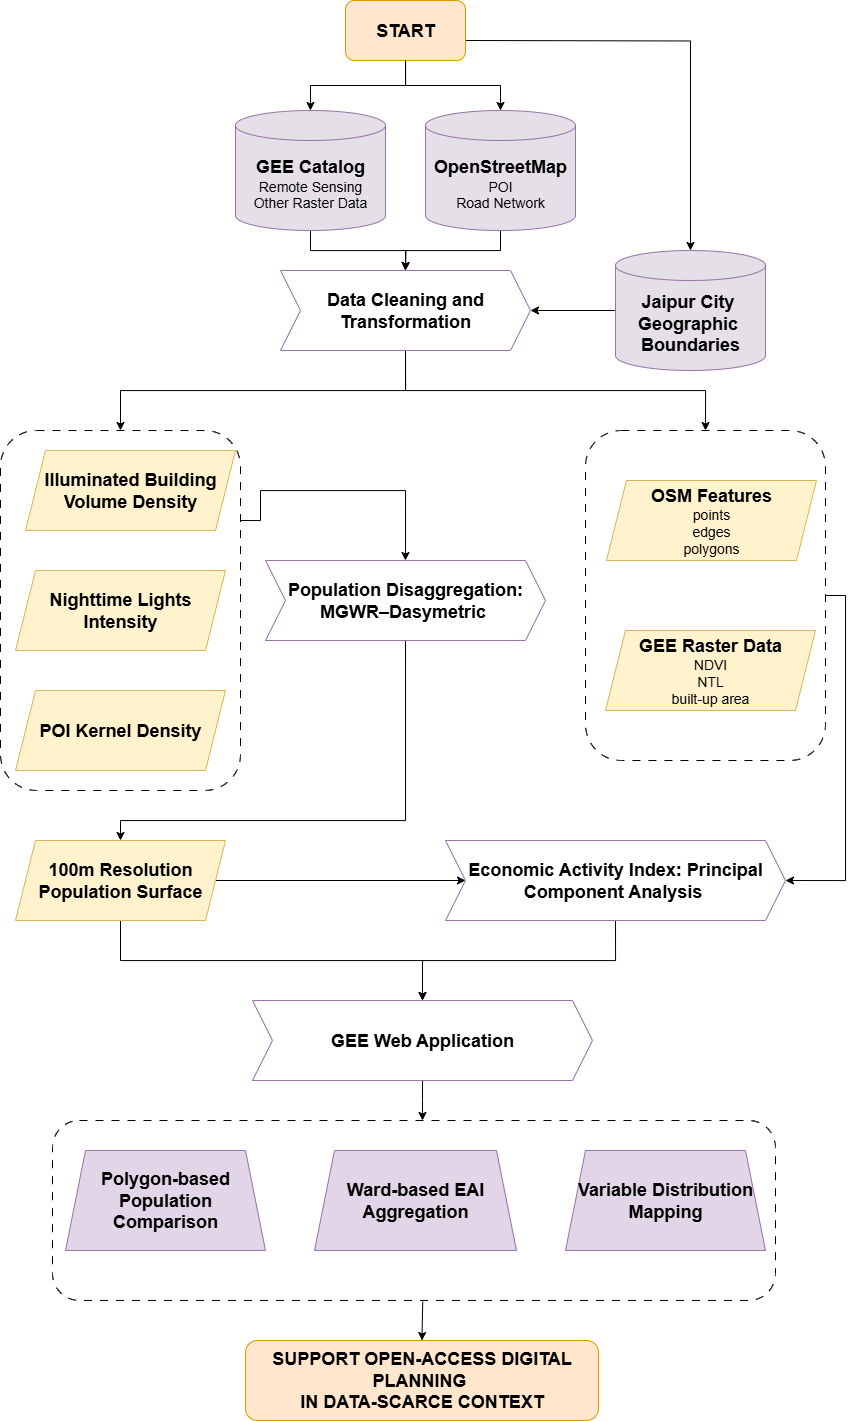
\includegraphics[width=0.8\linewidth]{thesis_images/03ME_flowchart} 

}

\caption{Methodology Flowchart }\label{fig:03ME-flowchart}
\end{figure}

\section{Study Area}\label{study-area}

This study focuses on Jaipur City, the political and economic centre of Rajasthan and one of the 100 cities nominated under India's Smart Cities Mission. While the wider Jaipur Development Authority (JDA) boundary covers a much larger territory, its constituent areas are defined by heterogeneous spatial units---wards in the city, but villages and small towns in the surrounding region; as a result, the combination of this mismatch and the absence of recent high-granularity population data for the non-urban areas makes it difficult to assemble a consistent dataset at the resolution required for this analysis. In contrast, the municipal area offers a uniform ward-based framework, enabling demographic, remote sensing, and open spatial datasets to be integrated on the same spatial level. Moreover, by focusing on this city boundary, the results directly align with ongoing municipal-level digital planning initiatives, where outputs can inform infrastructure monitoring, mobility management, and public service optimisation.

The analysis begins at the ward level, using the 250 wards managed by the Jaipur Municipal Corporation (JMC) as the basic spatial units. According to administrative estimates released by JDA in 2020, these wards collectively host a residential population of 3,053,908. Since the last official Indian census was conducted in 2011, this JDA estimates provide the most recent demographic baseline.

Jaipur's urban morphology comprises a dense, historic walled city at its core, encircled by peripheral areas that have expanded rapidly along major transport corridors. Together, these patterns combine compact heritage neighbourhoods with low-density, recently urbanised wards, creating a varied setting for analysing spatial heterogeneity in population distribution and economic activity.

The study area is shown in Figure \ref{fig:03ME-location}, where the JMC boundary is highlighted alongside internal ward divisions. This municipal extent therefore defines the spatial scope for all subsequent modelling and analysis steps.

\begin{figure}

{\centering 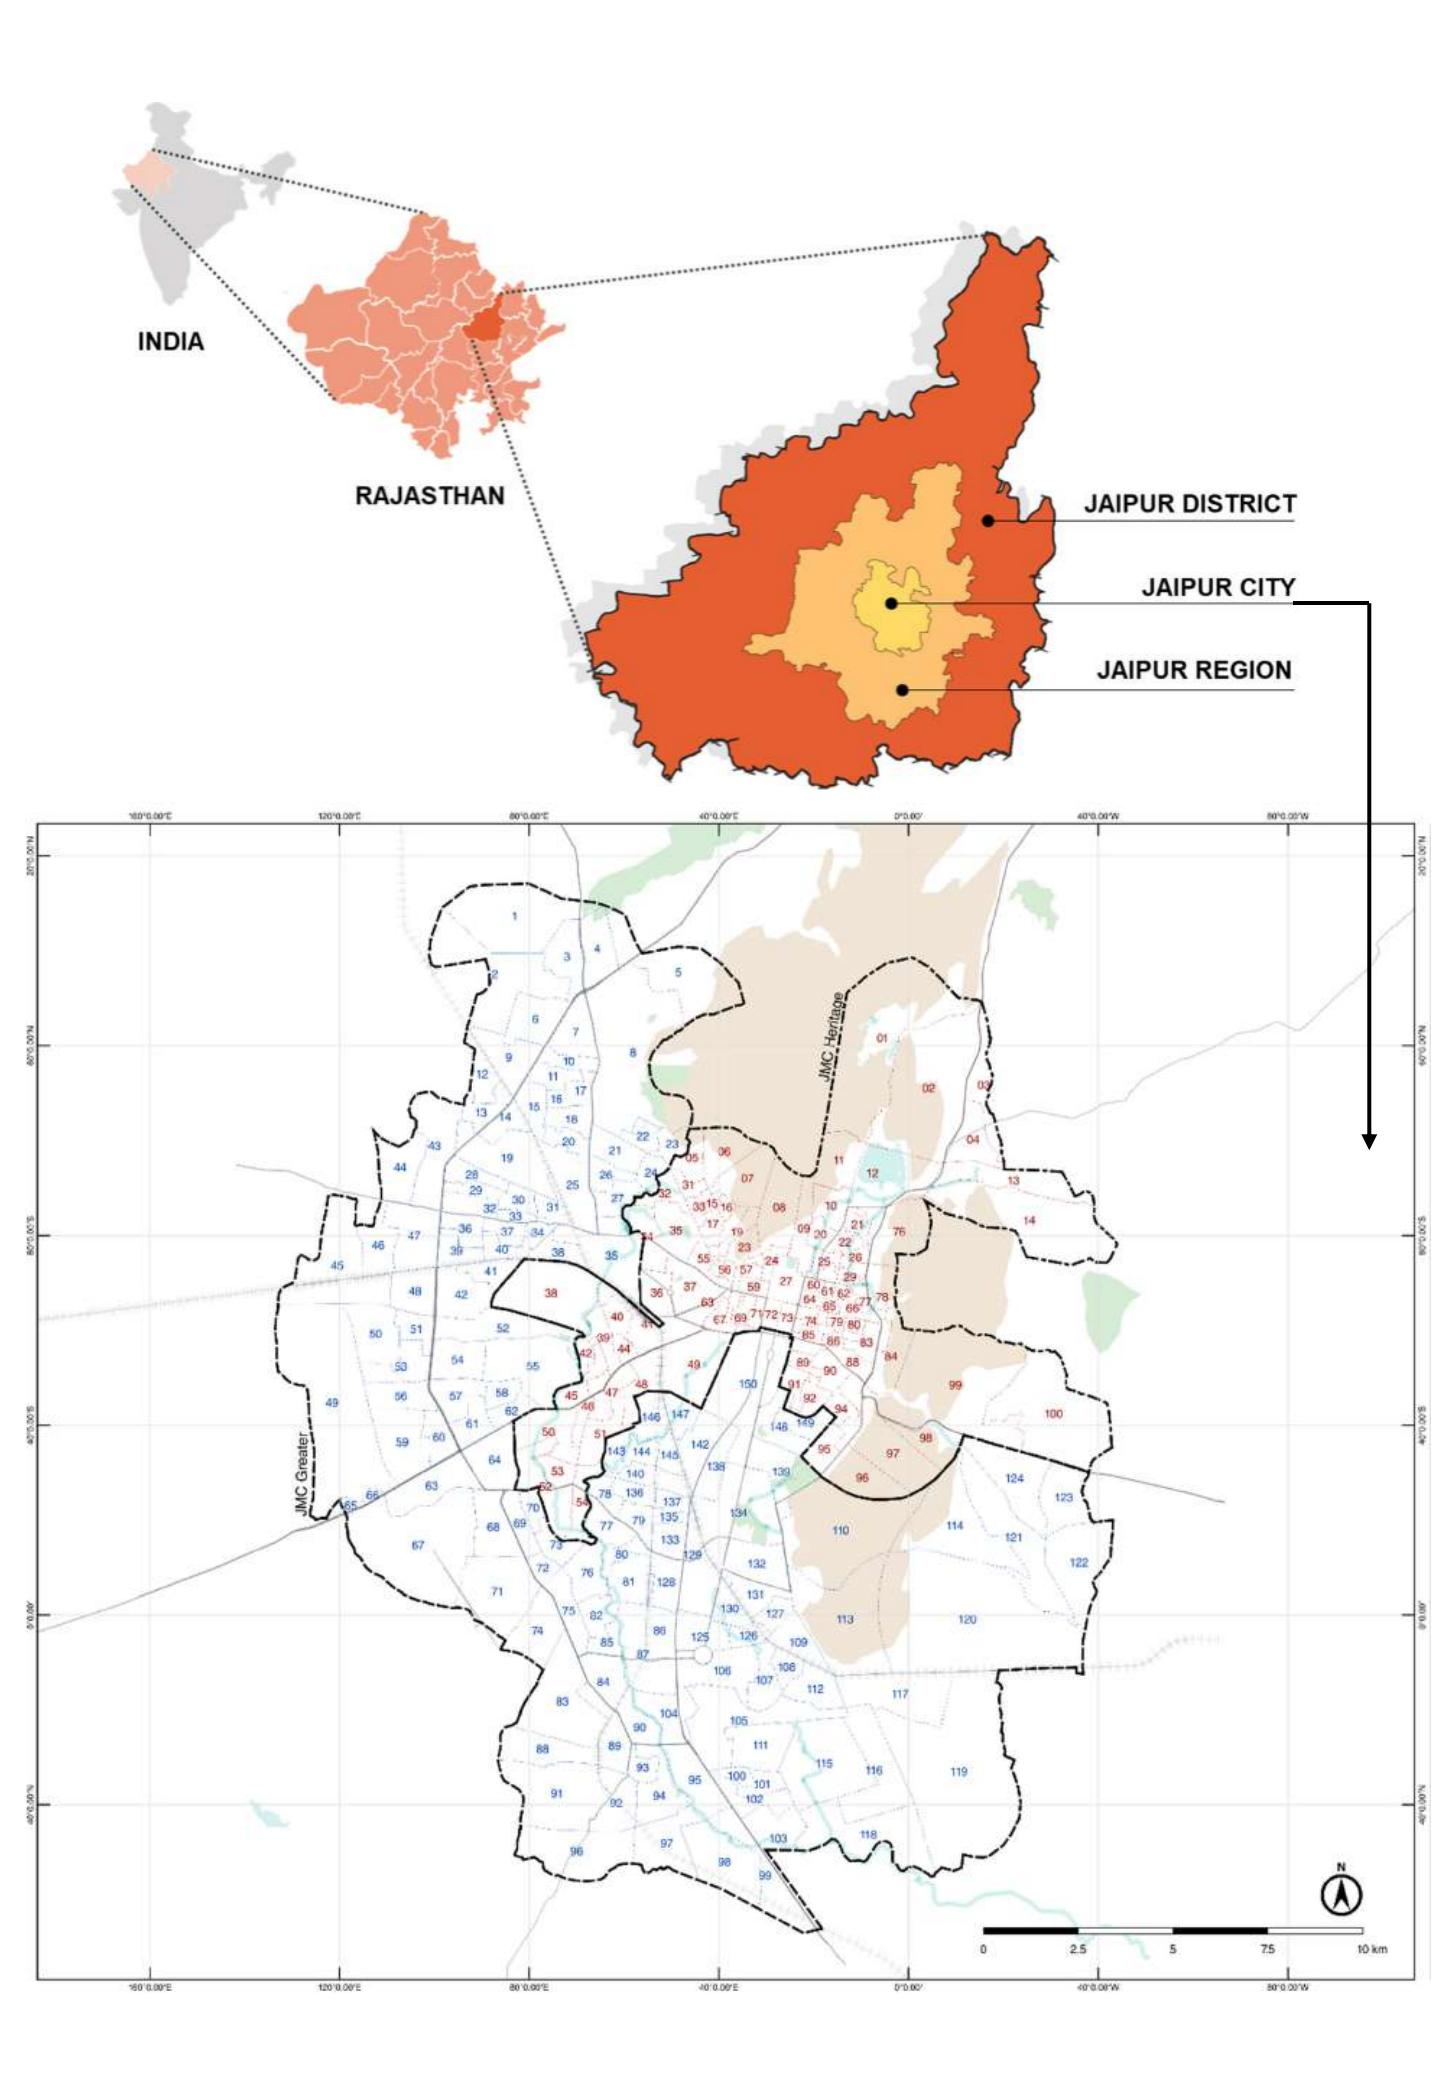
\includegraphics[width=0.9\linewidth]{thesis_images/03ME_location} 

}

\caption{ Location of Jaipur City. Source: UN-Habitat. }\label{fig:03ME-location}
\end{figure}

\section{Data Sources and Preparation}\label{data-sources-and-preparation}

The datasets used in this study were selected and prepared to match the requirements of the two main analytical stages: the MGWR--dasymetric hybrid approach for population disaggregation, and the PCA for constructing the EAI. Most datasets were obtained from open-access platforms, primarily the Google Earth Engine (GEE) Data Catalog and OpenStreetMap (OSM), except for the Jaipur City boundary and ward-level population data, which were provided by the Malaviya National Institute of Technology (MNIT) Jaipur.

\subsection{Data for MGWR}\label{data-for-mgwr}

The \textbf{dependent variable} in the MGWR model is \textbf{ward-level residential population density}, derived from JDA population estimates from 2020. Here, residential population refers to where people live, in contrast to ambient population, which captures where people may be present throughout the day (e.g.~workplaces, shopping areas, or transit hubs). Accordingly, all explanatory variables were masked to residential built-up areas, so that predictors reflect residential locations rather than other land uses \autocite{pesaresiAdvancesGlobalHuman2024a}. Detailed data sources are provided in Table \ref{tab:mgwr-variables}.

The selection of \textbf{explanatory variables} followed the four broad categories of ancillary data commonly used in population disaggregation---land cover, nighttime lights, infrastructure, and environmental factors \autocite{qiuDisaggregatingPopulationData2022}. Given that environmental variables such as elevation were excluded, the final set includes only the first three categories, all of which exhibited spatial patterns closely aligned with population distribution, with highest values concentrated in the historic walled city (Figure \ref{fig:03ME-mgwr-feature-maps} and Figure \ref{fig:03ME-mgwr-feature-his}):

\begin{enumerate}
\def\labelenumi{\arabic{enumi}.}
\item
  \textbf{Illuminated Building Volume Density} --- Estimated by multiplying the height of each residential built-up pixel from the GHSL settlement dataset by its area, then masking to areas illuminated in VIIRS nighttime lights imagery. In practice, all residential built-up areas in Jaipur were found to be illuminated, making additional filtering unnecessary. Heights were binned into ranges (e.g.~\textless3 m, 3--6 m) and assigned midpoint values (e.g.~1.5 m, 4.5 m). This midpoint approach introduces uncertainty, as the chosen values may not represent the actual height distribution, producing visible abrupt boundaries in the mapped volume variable.
\item
  \textbf{Nighttime Lights Intensity} --- Derived from VIIRS annual composites, averaged across the study period and log-transformed (log(x + 1)) to reduce skewness.
\item
  \textbf{POI Kernel Density} --- Calculated from OSM amenities POI that are relevant to residential life rather than including office-based or other employment-related POI which reflect ambient rather than residential population. Eight amenity categories (i.e.~education, entertainment, facilities, financial, healthcare, public service, sustenance, and transportation) were tested at ward level, but only sustenance, facilities and healthcare showed meaningful correlations with ward populations, so the others were excluded. The kernel bandwidth was set to 1600m because this value maximised the correlation between POI density and population counts. A detailed correlation matrix is provided in the Appendix.
\end{enumerate}

To improve model stability, both dependent and independent variables were transformed using log(x + 1), standardised to z-scores, and aggregated to the ward level before MGWR fitting. Also, all rasters were aligned to a 100 m grid and a common projection prior to modelling to ensure pixel-level consistency across datasets. Despite these preparations, the MGWR data stage has limitations. The exclusion of environmental factors such as elevation---despite substantial variation across wards---may reduce explanatory power. The use of midpoint values for height estimation can lead to artificial discontinuities in building volume, and the POI kernel density is dependent on the positional accuracy and completeness of OSM data.

\setlength{\tabcolsep}{4pt}

\begingroup\fontsize{8.8}{10.8}\selectfont

\begin{longtable}[t]{p{0.18\linewidth}p{0.35\linewidth}p{0.20\linewidth}p{0.27\linewidth}}
\caption{\label{tab:mgwr-variables}MGWR Model Variables: Definitions, Details and Data Sources}\\
\toprule
\textbf{Variable} & \textbf{Description} & \textbf{Details} & \textbf{Sources}\\
\midrule
\endfirsthead
\caption[]{\label{tab:mgwr-variables}MGWR Model Variables: Definitions, Details and Data Sources \textit{(continued)}}\\
\toprule
\textbf{Variable} & \textbf{Description} & \textbf{Details} & \textbf{Sources}\\
\midrule
\endhead

\endfoot
\bottomrule
\endlastfoot
illum vol density & Illuminated Building Volume Density: Illuminated building footprint volume per hectare within ward, masked by residential area & Available from band=['built characteristics Class Table'] & GHSL: Global settlement characteristics (10 m) 2018 (P2023A)\\
light intensity & Nighttime Lights Intensity: Mean annual DNB radiance within ward, masked by residential area & Available from band=['average'] & VIIRS Nighttime Day/Night Annual Band Composites V2.2 (2022-2024)\\
POI KD & POI Kernel Density: Mean POI kernel density within ward, masked by residential area & Available from OSM POI (amenity=*) & OpenStreetMap (2025)\\
POP density & Pop Density: Population density per hectare within ward & Available from col=['POP'] & JDA Population Estimates (2020)\\*
\end{longtable}
\endgroup{}

\setlength{\tabcolsep}{6pt}

\begin{figure}

{\centering 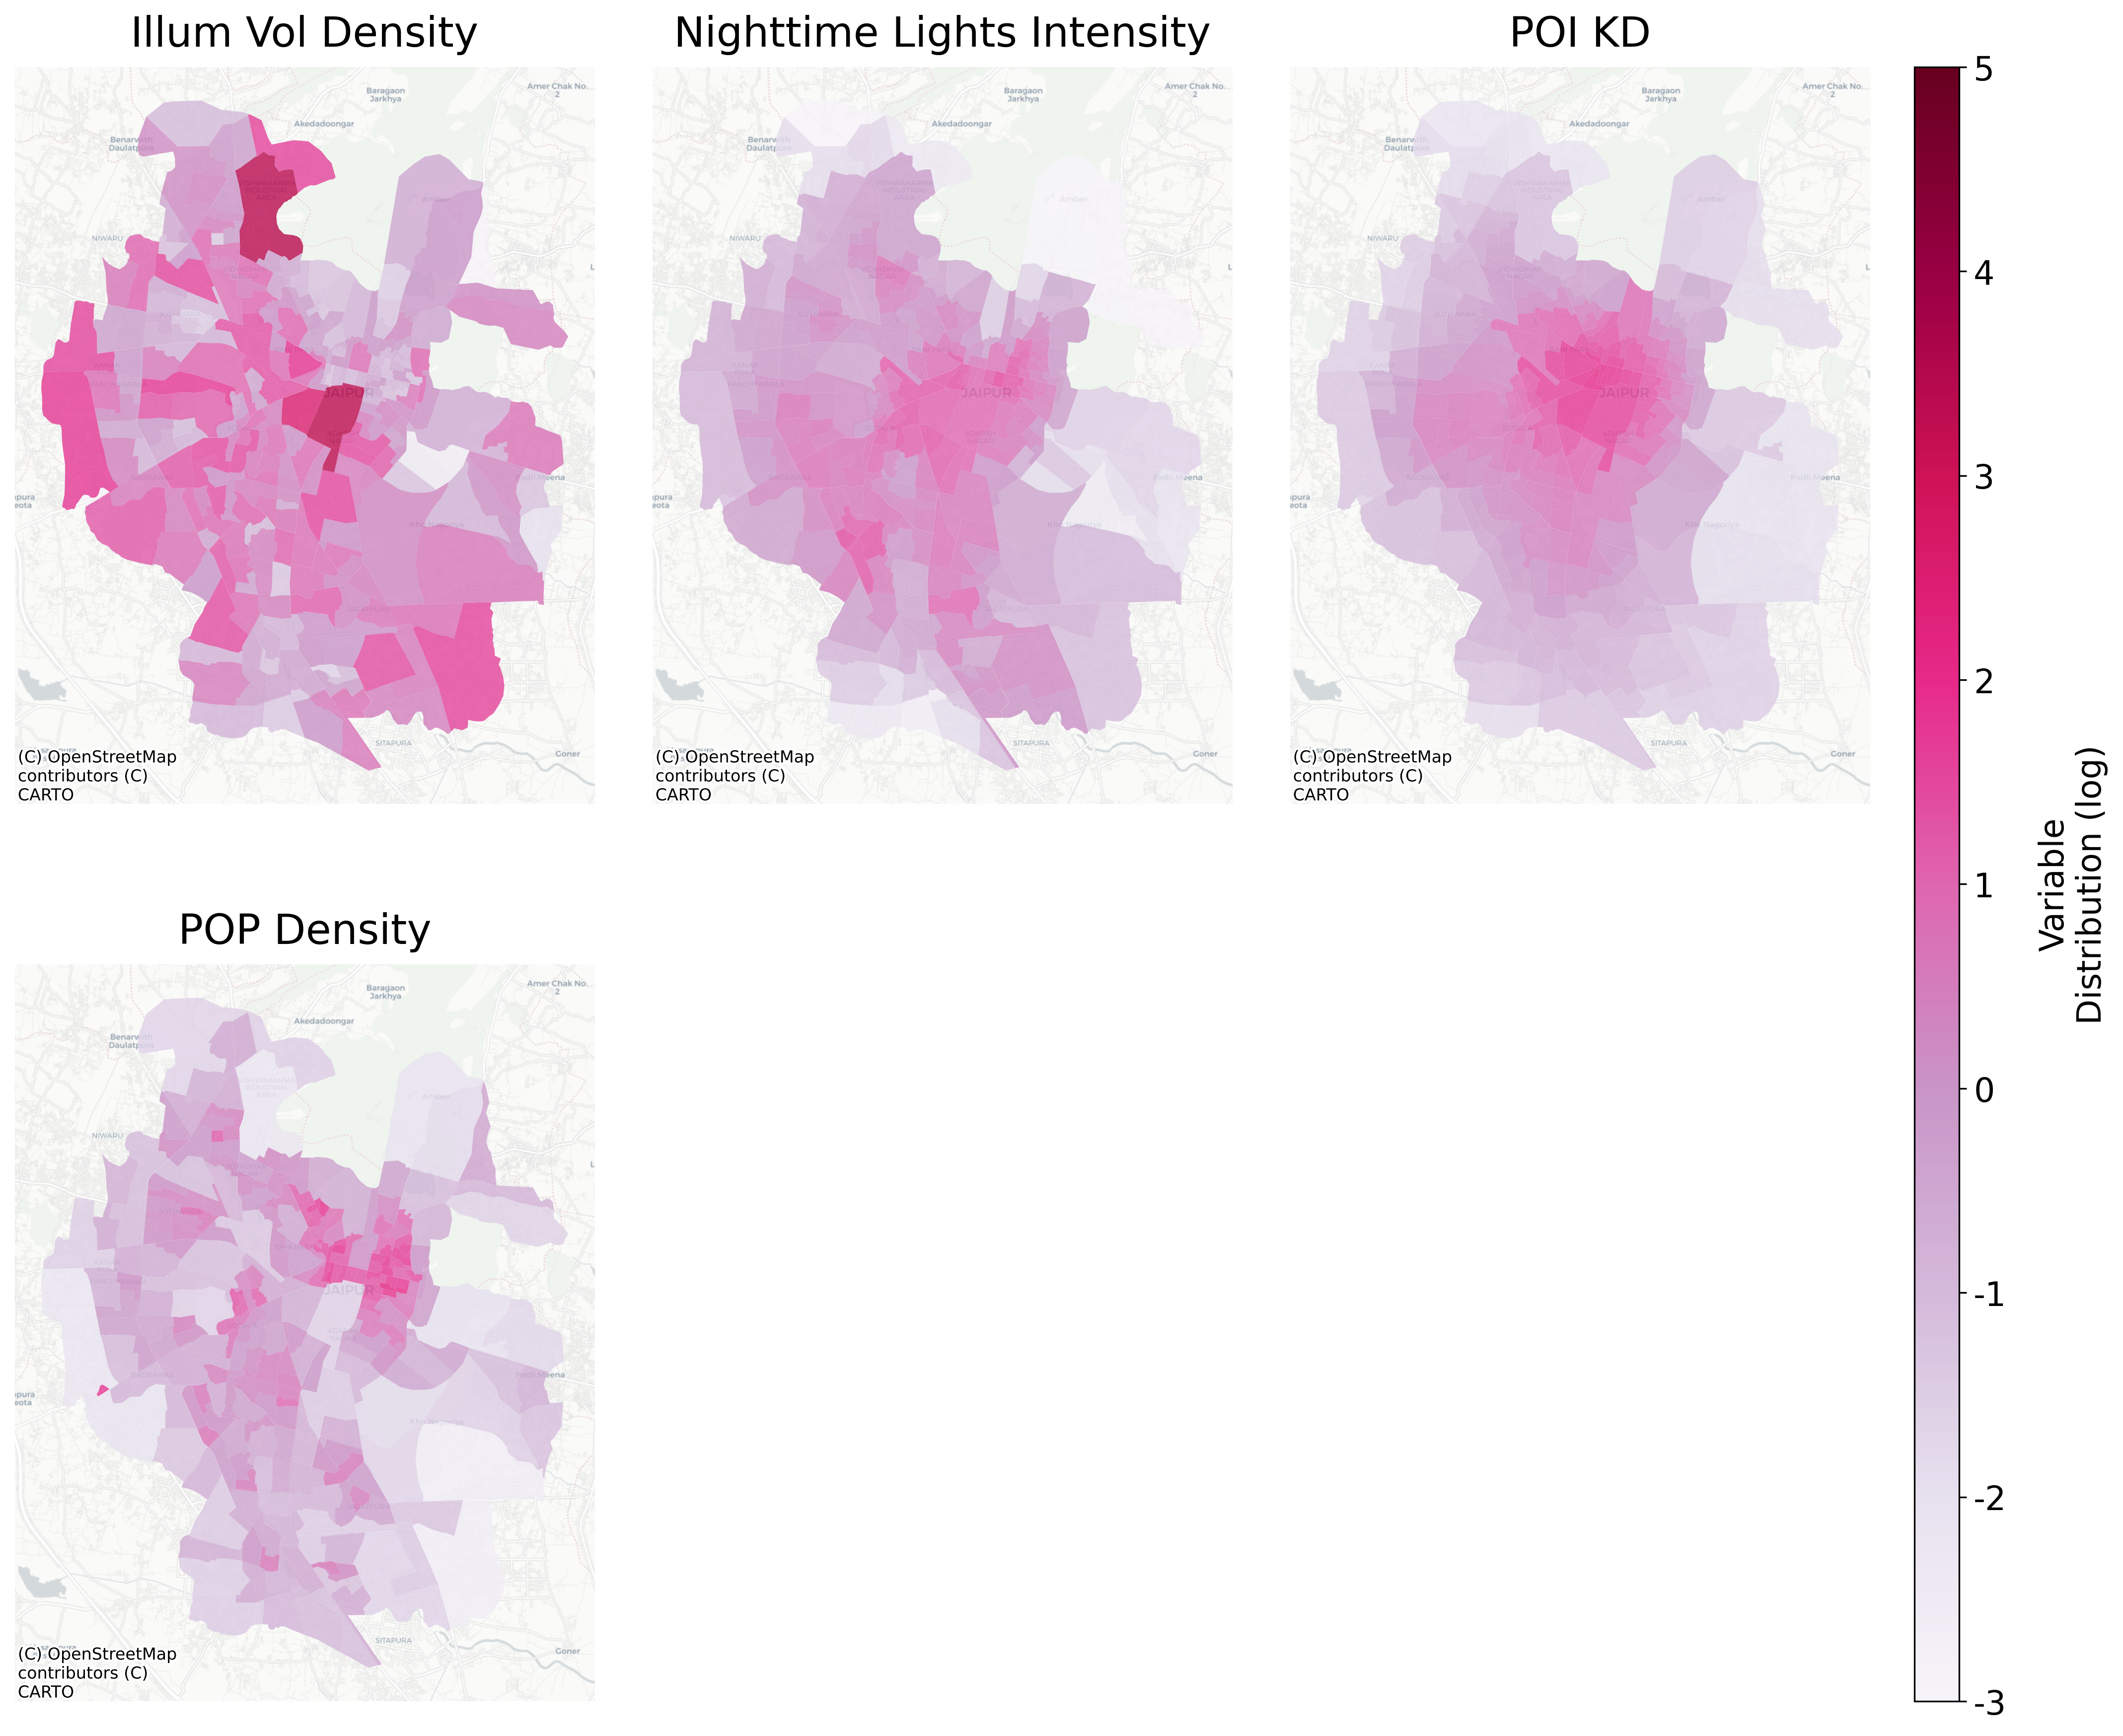
\includegraphics[width=0.9\linewidth]{thesis_images/03ME_mgwr_feature_maps} 

}

\caption{ MGWR Model Variables Distribution (after log and z-score transformation) }\label{fig:03ME-mgwr-feature-maps}
\end{figure}

\begin{figure}

{\centering 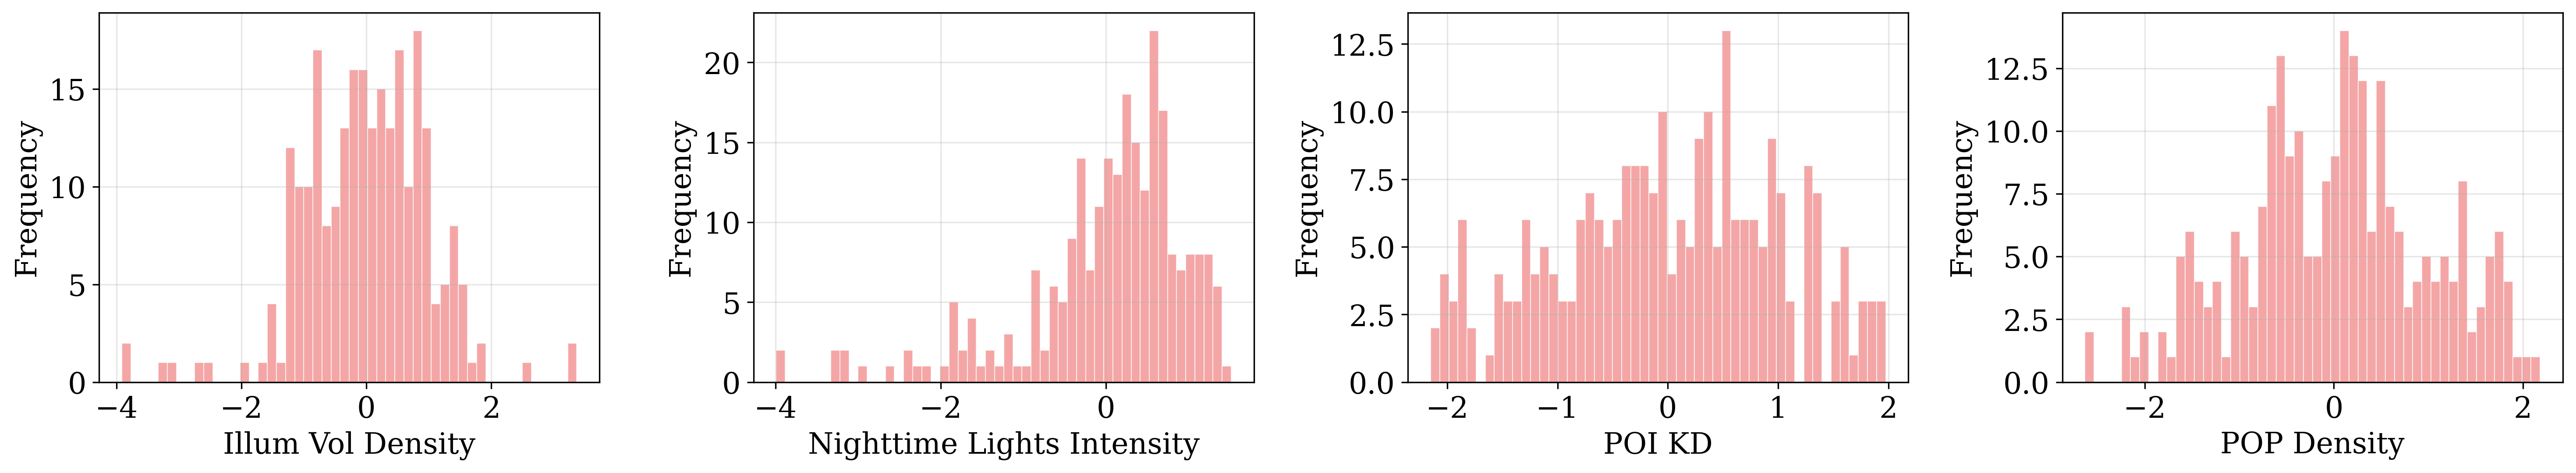
\includegraphics[width=0.9\linewidth]{thesis_images/03ME_mgwr_trans_var} 

}

\caption{ MGWR model Variables Distribution Histogram (after log and z-score transformation) }\label{fig:03ME-mgwr-feature-his}
\end{figure}

\subsection{Data for PCA}\label{data-for-pca}

The PCA stage combines residential population density, derived from the 100 m disaggregated raster produced by the MGWR--dasymetric process (converted to population density in km²), with a set of spatial indicators describing built environment characteristics and accessibility. Together, these indicators can indirectly reflect the presence of economic activity, as many have been used in prior studies to approximate metrics such as employment density \autocite{barzinWhereAreAll2022a}.While residential density is not a direct measure of economic activity, it reflects demand-side dynamics (where people live and consume), and its limitations are balanced by other indicators that capture supply-side and ambient factors such as workplaces, services, and infrastructure.

All datasets (Table \ref{tab:pca-variables}) were aggregated to a 500 m hexagonal grid (point spacing), transformed using log(x + 1) to reduce skewness, and standardised to z-scores before PCA input. NDVI was excluded from the log transformation because its values are already normalised to a fixed range. From the distribution maps (Figure \ref{fig:03ME-pca-feature-maps} and Figure \ref{fig:03ME-pca-feature-his}), these variables reveal a clear pattern of urban expansion from the walled city towards the west, with the eastern mountains acting as a natural barrier to urban growth.

The PCA indicators come from two main sources:

\begin{enumerate}
\def\labelenumi{\arabic{enumi}.}
\item
  \textbf{Vector data from OSM} --- Points (e.g.~amenities), lines (e.g.~road networks), and polygons (e.g.~large transport stations such as the airport) were converted into density measures---counts, lengths, or areas per square kilometre---within each hexagon. For hexagons intersecting the municipal boundary, only the area inside the boundary was used to compute density, ensuring accurate representation in edge cells.
\item
  \textbf{Raster data from GEE} --- Datasets such as NDVI and VIIRS NTL were averaged over time before aggregation to the 500 m grid. For sum-based measures (e.g.~population, built-up area), values were divided by the actual area of each hexagon within the municipal boundary to avoid underestimation in partially covered cells.
\end{enumerate}

\setlength{\tabcolsep}{4pt}

\begingroup\fontsize{8.8}{10.8}\selectfont

\begin{longtable}[t]{p{0.18\linewidth}p{0.30\linewidth}p{0.25\linewidth}p{0.27\linewidth}}
\caption{\label{tab:pca-variables}PCA Variables: Definitions, Details and Data Sources}\\
\toprule
\textbf{Variable} & \textbf{Description} & \textbf{Details} & \textbf{Sources}\\
\midrule
\endfirsthead
\caption[]{\label{tab:pca-variables}PCA Variables: Definitions, Details and Data Sources \textit{(continued)}}\\
\toprule
\textbf{Variable} & \textbf{Description} & \textbf{Details} & \textbf{Sources}\\
\midrule
\endhead

\endfoot
\bottomrule
\endlastfoot
builtup density & Built-up Area: Built-up surface per km² & Available from band=['built surface'] & GHSL: Global built-up surface 2020 (P2023A)\\
ntl mean & Nighttime Lights: Mean annual DNB radiance within hexagon & Available from band=['average'] & VIIRS Nighttime Day/Night Annual Band Composites V2.2 (2022-2024)\\
pop density km2 & Population: Population surface per km² & Derived from MGWR 100m resolution population counts surface & See data sources of MGWR stage\\
motorable road network & Motorable Road: Length of major road network per km² & Available from OSM road hierarchy (highway=*, e.g. trunk, primary) & OpenStreetMap (2025)\\
amenities poi & Amenities: Count of amenities POI per km² & Available from OSM POI (amenity=*) & OpenStreetMap (2025)\\
\addlinespace
shop poi & Shops: Count of shops POI per km² & Available from OSM POI (shop=*) & OpenStreetMap (2025)\\
transport station point & Transport Station: Count of transport nodes (e.g. bus stops) per km² & Available from OSM Transport POI (public transport, railway, amenity, highway, aeroway tags; points and linestrings only) & OpenStreetMap (2025)\\
office poi & Offices: Count of offices POI per km² & Available from OSM POI (office=*) & OpenStreetMap (2025)\\
transport station polygon & Transport Station (large): Area of large transport facilities (e.g. airport) per km² & Available from OSM Transport POI (public transport, railway, amenity, highway, aeroway tags; polygons only) & OpenStreetMap (2025)\\
ndvi mean & NDVI: Mean Daily Normalised Difference Vegetation within hexagon & Available from band=['SR B4', 'SR B5'] & Landsat 9 Level 2, Collection 2, Tier 1 (2023-2024)\\*
\end{longtable}
\endgroup{}

\setlength{\tabcolsep}{6pt}

\begin{figure}

{\centering 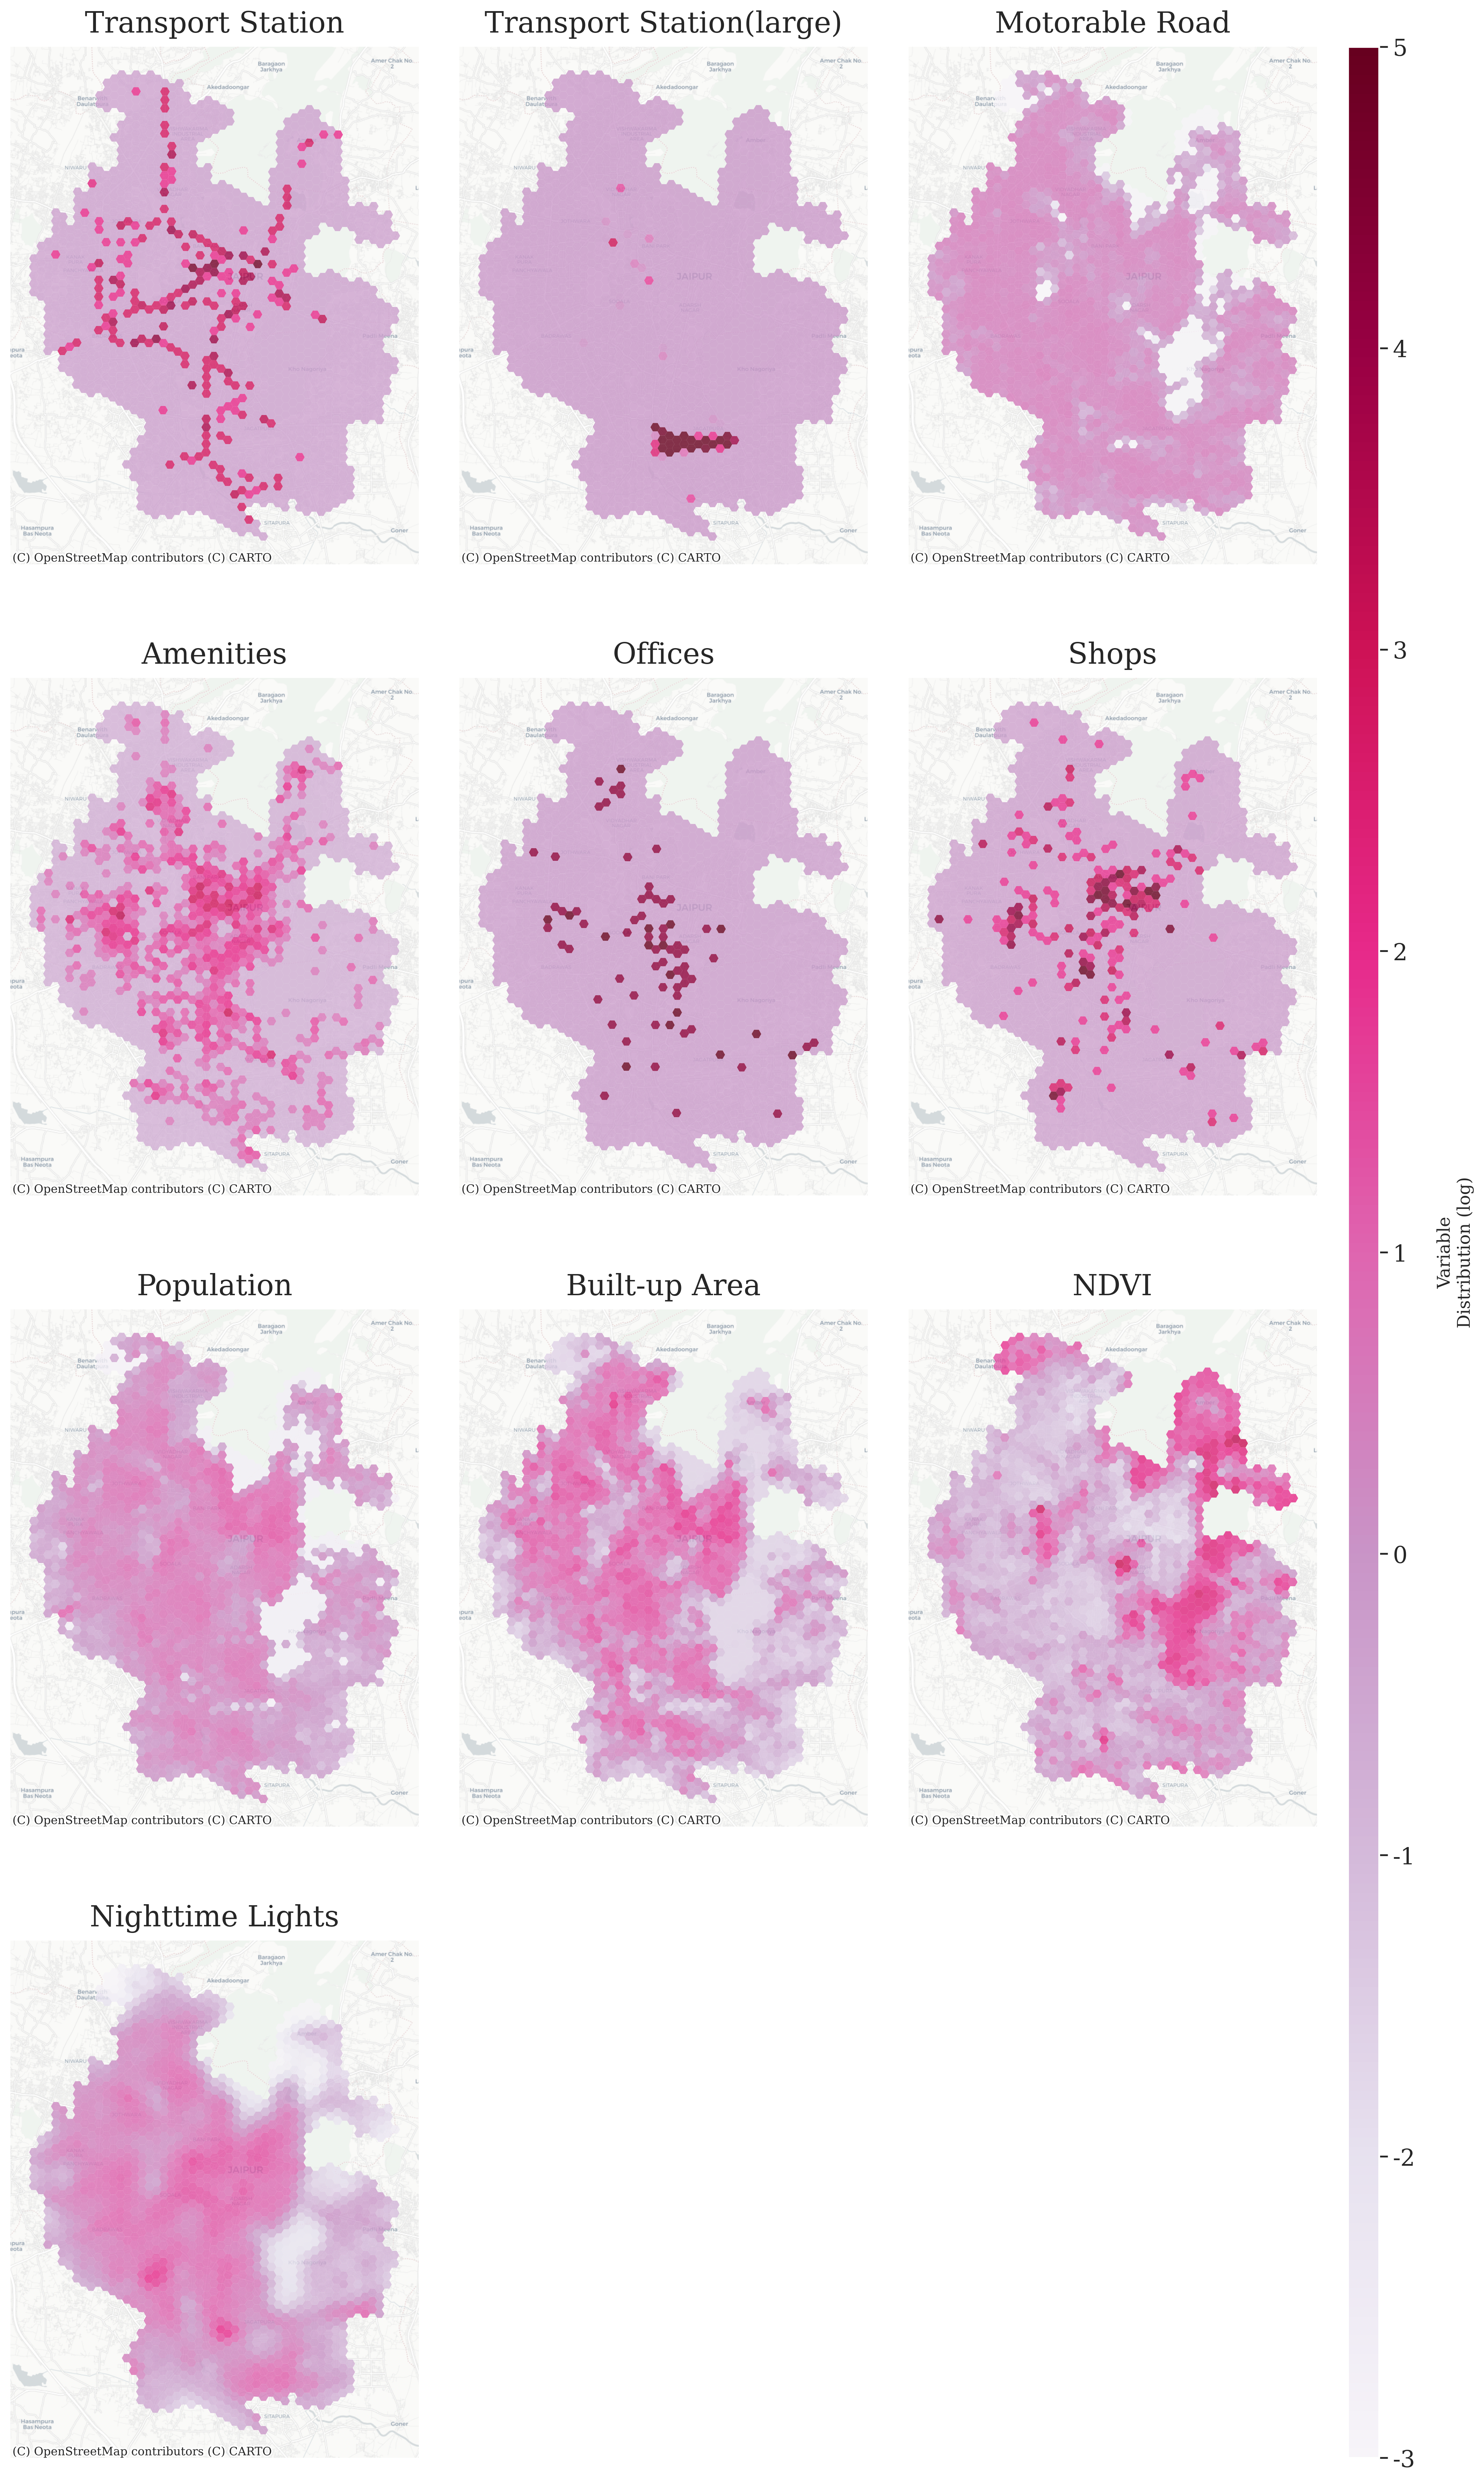
\includegraphics[width=0.9\linewidth]{thesis_images/03ME_indicator_maps} 

}

\caption{ PCA Variables Distribution (after log and z-score transformation) }\label{fig:03ME-pca-feature-maps}
\end{figure}

\begin{figure}

{\centering 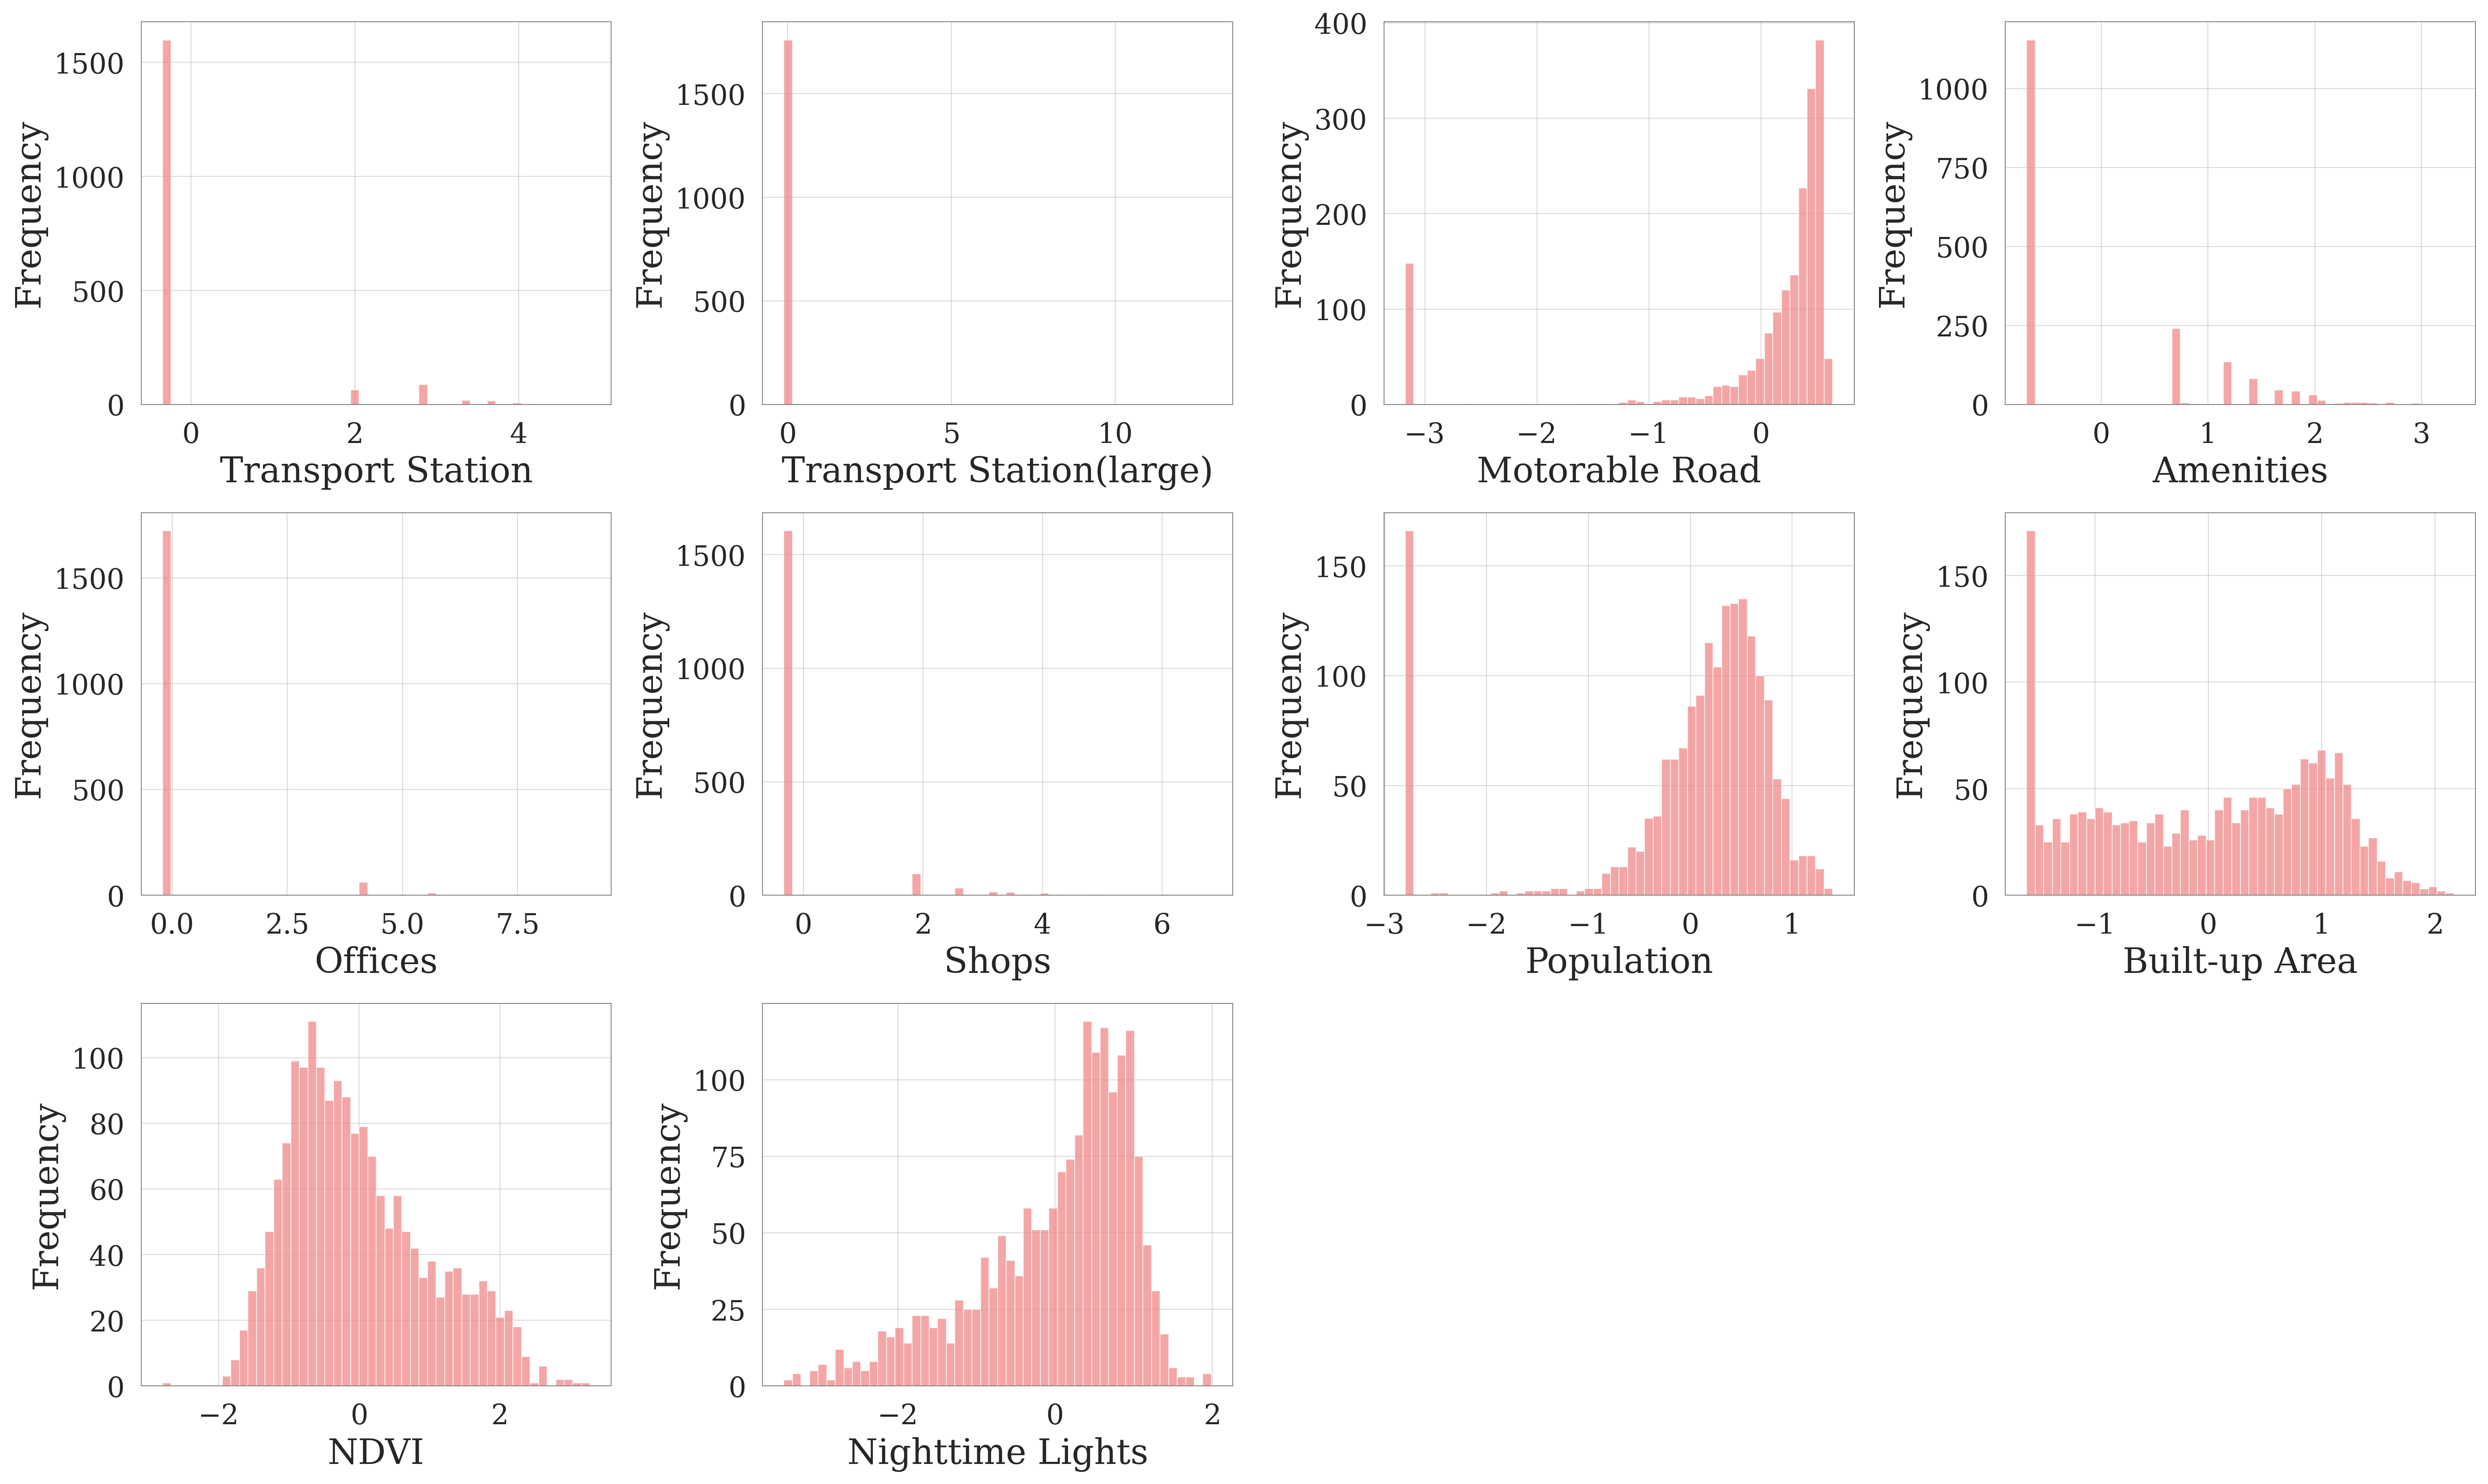
\includegraphics[width=0.9\linewidth]{thesis_images/03ME_standardized_indicators_histograms} 

}

\caption{ PCA Variables Distribution Histogram (after log and z-score transformation) }\label{fig:03ME-pca-feature-his}
\end{figure}

\section{Population Disaggregation: MGWR--Dasymetric Hybrid Approach}\label{population-disaggregation-mgwrdasymetric-hybrid-approach}

In contexts where high-resolution population data are unavailable, combining statistical modelling with dasymetric mapping can improve the spatial accuracy of population estimates \autocite{pajaresPopulationDisaggregationBuilding2021,sapenaEmpiricRecommendationsPopulation2022}. In Jaipur, the absence of an official census since 2011 and reliance on JDA ward-level estimates from 2020 further necessitate such approaches, as they allow recent population values to be inferred at sufficient spatial granularity. In this study, the Multiscale Geographically Weighted Regression (MGWR) model was used to capture the spatially varying relationships between Jaipur ward-level residential population density and multiple environmental predictors, while the dasymetric mask constrained the disaggregation of population counts only to residential built-up areas.

MGWR extends the traditional GWR framework by allowing not only regression coefficients to vary across space, but also the spatial scale at which each explanatory variable operates. This is achieved by estimating separate bandwidths for each variable, enabling the integration of predictors that influence population patterns over large spatial scales (e.g.~regional accessibility) with those operating at finer scales (e.g.~building volume density).

Let:

\begin{itemize}
\tightlist
\item
  \(P_w\) = ward-level residential population density
\item
  \(P_g\) = grid-level residential population density
\item
  \(V\) = illuminated building volume density
\item
  \(L\) = VIIRS nighttime light intensity
\item
  \(K\) = POI kernel density
\item
  \(V_g, L_g, K_g\) = corresponding variables at the grid level
\item
  \(w_g\) = adjusted weight for grid \(g\) in ward \(w\)
\end{itemize}

The ward-level MGWR model is:

\begin{equation} 
  \log(P_w + 1) = \beta_0(u,v) + \beta_V(u,v) \, V + \beta_L(u,v) \, L + \beta_K(u,v) \, K + \varepsilon
  \label{eq:MWGRward}
\end{equation}

The MGWR was implemented in Python using the \emph{mgwr} package, with ward centroids used to compute inter-ward distances. A Gaussian kernel was employed, and optimal bandwidths for each predictor were determined using the golden section search to minimise the corrected Akaike Information Criterion (AICc). All explanatory variables were masked to residential built-up areas, log-transformed as \(\log(x+1)\), and standardised to z-scores prior to modelling.

Ward-level MGWR coefficients were then applied to grid-level raster layers, producing 100 m resolution predictions:

\begin{equation} 
\widehat{\log(P_g + 1)} = \hat{\beta}_0(u,v) + \hat{\beta}_V(u,v) \, V_g + \hat{\beta}_L(u,v) \, L_g + \hat{\beta}_K(u,v) \, K_g
  \label{eq:MWGRgrid}
\end{equation}

These predictions are grid-level log-scale estimates (\(\widehat{\log(P_g+1)}\)). Because coefficients are ward-specific, we treat them as within-ward scores and, within each ward, convert them to disaggregation weights using min--max normalisation and a Softmax-based allocation with a smoothing transform (summing to 1), followed by \(\alpha\)-power shrinkage and 99th-percentile winsorisation. This balances the dominance of peak cells while preserving local contrasts. The code implementing this transformation is provided in the Appendix.

Finally, the ward-level population totals were disaggregated to the 100 m grids according to these adjusted weights:

\begin{equation} 
P_g = \frac{w_g}{\sum_{g \in w} w_g} \times P_w
  \label{eq:POPweights}
\end{equation}

The resulting grid-level counts were integerised to ensure exact ward-level totals. The final output is a 100 m resolution residential population raster for Jaipur City.

\section{Economic Activity Index: Principal Component Analysis Approach}\label{economic-activity-index-principal-component-analysis-approach}

In the second analytical stage, multiple spatial indicators are integrated into a single measure of economic activity using Principal Component Analysis (PCA). PCA is widely applied in composite index construction for its ability to transform correlated inputs into independent components, allowing the main patterns of variation to be summarised while avoiding overweighting information repeated across indicators \autocite{vyasConstructingSocioeconomicStatus2006a,conlonMappingHumanVulnerability2020}. In contrast to equal weighting or expert judgement, PCA derives variable weights directly from the data, giving greater influence to indicators that contribute more to the shared variance \autocite{brobyUsePrincipalComponents2022a}.

This approach is particularly suitable for this study. The selected spatial indicators---derived from built environment characteristics, accessibility measures, and other spatial variables linked to economic activity---are theoretically connected and empirically correlated based on reviewed literature, suggesting the presence of a common latent dimension. Retaining the first principal component (PC1) provides a data-driven way to capture the overall spatial intensity of economic activities without relying on manually assigned indicator weights.

PCA was applied to the standardised 500 m hexagon-level indicator matrix prepared in Section 3.2.2. PC1 was extracted based on the proportion of variance it explained and the interpretability of its loadings. The Economic Activity Index (EAI) for each hexagon \(i\) was calculated as:

\begin{equation} 
  \text{EAI}_i = \frac{\text{PC1}_i - \mu_{\text{PC1}}}{\sigma_{\text{PC1}}}
  \label{eq:EAI}
\end{equation}

where \(\mu_{\text{PC1}}\) and \(\sigma_{\text{PC1}}\) are the mean and standard deviation of the PC1 scores across all hexagons. This standardisation ensures comparability across space. The EAI values were subsequently examined using K-means clustering to identify distinct patterns of economic activity.

While PCA produces statistically optimal combinations of variables, its components are abstract and may not fully preserve the interpretability of the original measures and this trade-off is considered in the Discussion chapter.

\section{Integration into GEE Web Application}\label{integration-into-gee-web-application}

The population surface generated from the MGWR--dasymetric disaggregation and the hexagon-level Economic Activity Index (EAI) derived from the PCA stage were uploaded to the Google Earth Engine (GEE) asset repository. The population layer was provided as a raster, while the EAI was initially uploaded as a vector dataset and subsequently rasterised within GEE to support visualisation and ward-level aggregation. All assets were assigned public read permissions, enabling them to be accessed through their asset IDs.

The interactive application was developed using the GEE JavaScript API, with three main functions:

\begin{enumerate}
\def\labelenumi{\arabic{enumi}.}
\tightlist
\item
  \textbf{Polygon-based Population Comparison} -- Users can draw two polygons within the study area to aggregate population counts and visualise the results as a histogram.
\item
  \textbf{Ward-based EAI Aggregation} -- Users can aggregate the EAI by ward boundaries and view a ranked list of the top 10 wards, displaying official ward numbers and index values.
\item
  \textbf{Variable Distribution Mapping} -- Users can view thematic maps showing the spatial distribution of variables contributing to the EAI, using consistent symbology and classification for comparability.
\end{enumerate}

Once the code was completed, the application was published directly from the GEE Code Editor as a shareable web app, allowing stakeholders to access and interact with the outputs without needing specialised GIS software.

\section{Ethical Considerations}\label{ethical-considerations}

All datasets used in this study are either openly accessible or provided under institutional permission. Their use complies with the relevant licensing terms and collaborative agreements.

Potential privacy risks are mitigated by restricting the analysis to aggregated datasets, reporting population estimates at a 100 m grid resolution, and excluding any personally identifiable information. This resolution is sufficient for identifying broad spatial patterns while preventing the recognition of individual households or persons.

Nevertheless, the use of volunteered geographic information (VGI)---specifically OSM---introduces potential biases due to uneven contributor coverage, positional inaccuracies, and varying temporal completeness. Such biases may affect the representativeness of the input indicators, which in turn could influence the population surface and the Economic Activity Index (EAI). Furthermore, making the outputs publicly available through a GEE application may result in areas with high population density or elevated EAI receiving disproportionate attention from policymakers, businesses, or other stakeholders. While increased visibility can support digital planning, it may also risk reinforcing spatial inequalities if interpreted without adequate socio-economic context.

To address these concerns, this study documents all data sources, methodological choices, and limitations in detail, and reflects on these issues in the Discussion chapter. This transparency is intended to encourage responsible and context-aware use of the outputs in public planning and policy-making processes, while also filling critical data gaps in a data-scarce context and supporting planners with open-data-based, computational insights for more sustainable and inclusive urban development.

\chapter{Results}\label{results}

\section{Response to RQ1: Where People Live -- Population Estimation}\label{response-to-rq1-where-people-live-population-estimation}

\subsection{MGWR Model Performance}\label{mgwr-model-performance}

To justify the use of a local approach, the Multi-scale Geographically Weighted Regression (MGWR) was benchmarked against a global Ordinary Least Squares (OLS) model. As shown in Table \ref{tab:modelcomparison}, MGWR provides a substantially better fit, with an Adjusted \(R^{2}\) of 0.789 compared to 0.668 for OLS, and an AICc of 364.814 versus 442.420. The ΔAICc of 77.6 decisively favors MGWR, confirming its suitability for disaggregating population in Jaipur.

\setlength{\tabcolsep}{4pt}

\begingroup\fontsize{8.8}{10.8}\selectfont

\begin{longtable}[t]{p{2.5cm}rrp{8cm}}
\caption{\label{tab:modelcomparison}Comparative Performance Metrics of Global OLS and MGWR}\\
\toprule
\textbf{Metric} & \textbf{OLS} & \textbf{MGWR} & \textbf{Interpretation}\\
\midrule
\endfirsthead
\caption[]{\label{tab:modelcomparison}Comparative Performance Metrics of Global OLS and MGWR \textit{(continued)}}\\
\toprule
\textbf{Metric} & \textbf{OLS} & \textbf{MGWR} & \textbf{Interpretation}\\
\midrule
\endhead

\endfoot
\bottomrule
\endlastfoot
R² & 0.672 & 0.817 & Preliminary measure of fit; higher values indicate improved fit but can be inflated in local models.\\
Adjusted R² & 0.668 & 0.789 & Normalizes for model complexity; MGWR demonstrates superior explanatory performance.\\
AICc & 442.420 & 364.814 & Most reliable indicator; ΔAICc = 77.594 decisively favors MGWR (lower is better).\\*
\end{longtable}
\endgroup{}

\setlength{\tabcolsep}{6pt}

Beyond global fit indices, diagnostic checks confirmed the validity of the model. Moran's I on MGWR residuals (\(I = 0.0624, p = 0.0822\)) indicated no significant global spatial autocorrelation. The residual map (Figure \ref{fig:04RE-residual}), however, reveals localized patterns: central wards show balanced predictions, while the east and southeast display areas of systematic overestimation and the north--northeast shows systematic underestimation. Western districts present a fragmented mix of positive and negative residuals, highlighting local instability in model performance.

Further regression diagnostics reinforced these findings. The residual--fitted scatterplot demonstrated homoscedasticity, while the Q--Q plot indicated that the residuals follow an approximately normal distribution (Figure \ref{fig:04RE-residual-diagnostics}).

An assessment of local multicollinearity using the Condition Number (CN) revealed that values across most of the study area ranged from 2 to 8, indicating stable parameter estimates. Although some central locations exhibited moderate CN values (10--17), these remain well below the critical threshold of 30 that signals severe collinearity, confirming that multicollinearity is not a substantive concern in the model(Figure \ref{fig:04RE-CN}). In summary, the comparison with OLS and the full set of diagnostic checks confirm that MGWR is both statistically robust and spatially reliable, providing confidence in using its outputs as the basis for high-resolution population mapping in Jaipur.

\begin{figure}

{\centering 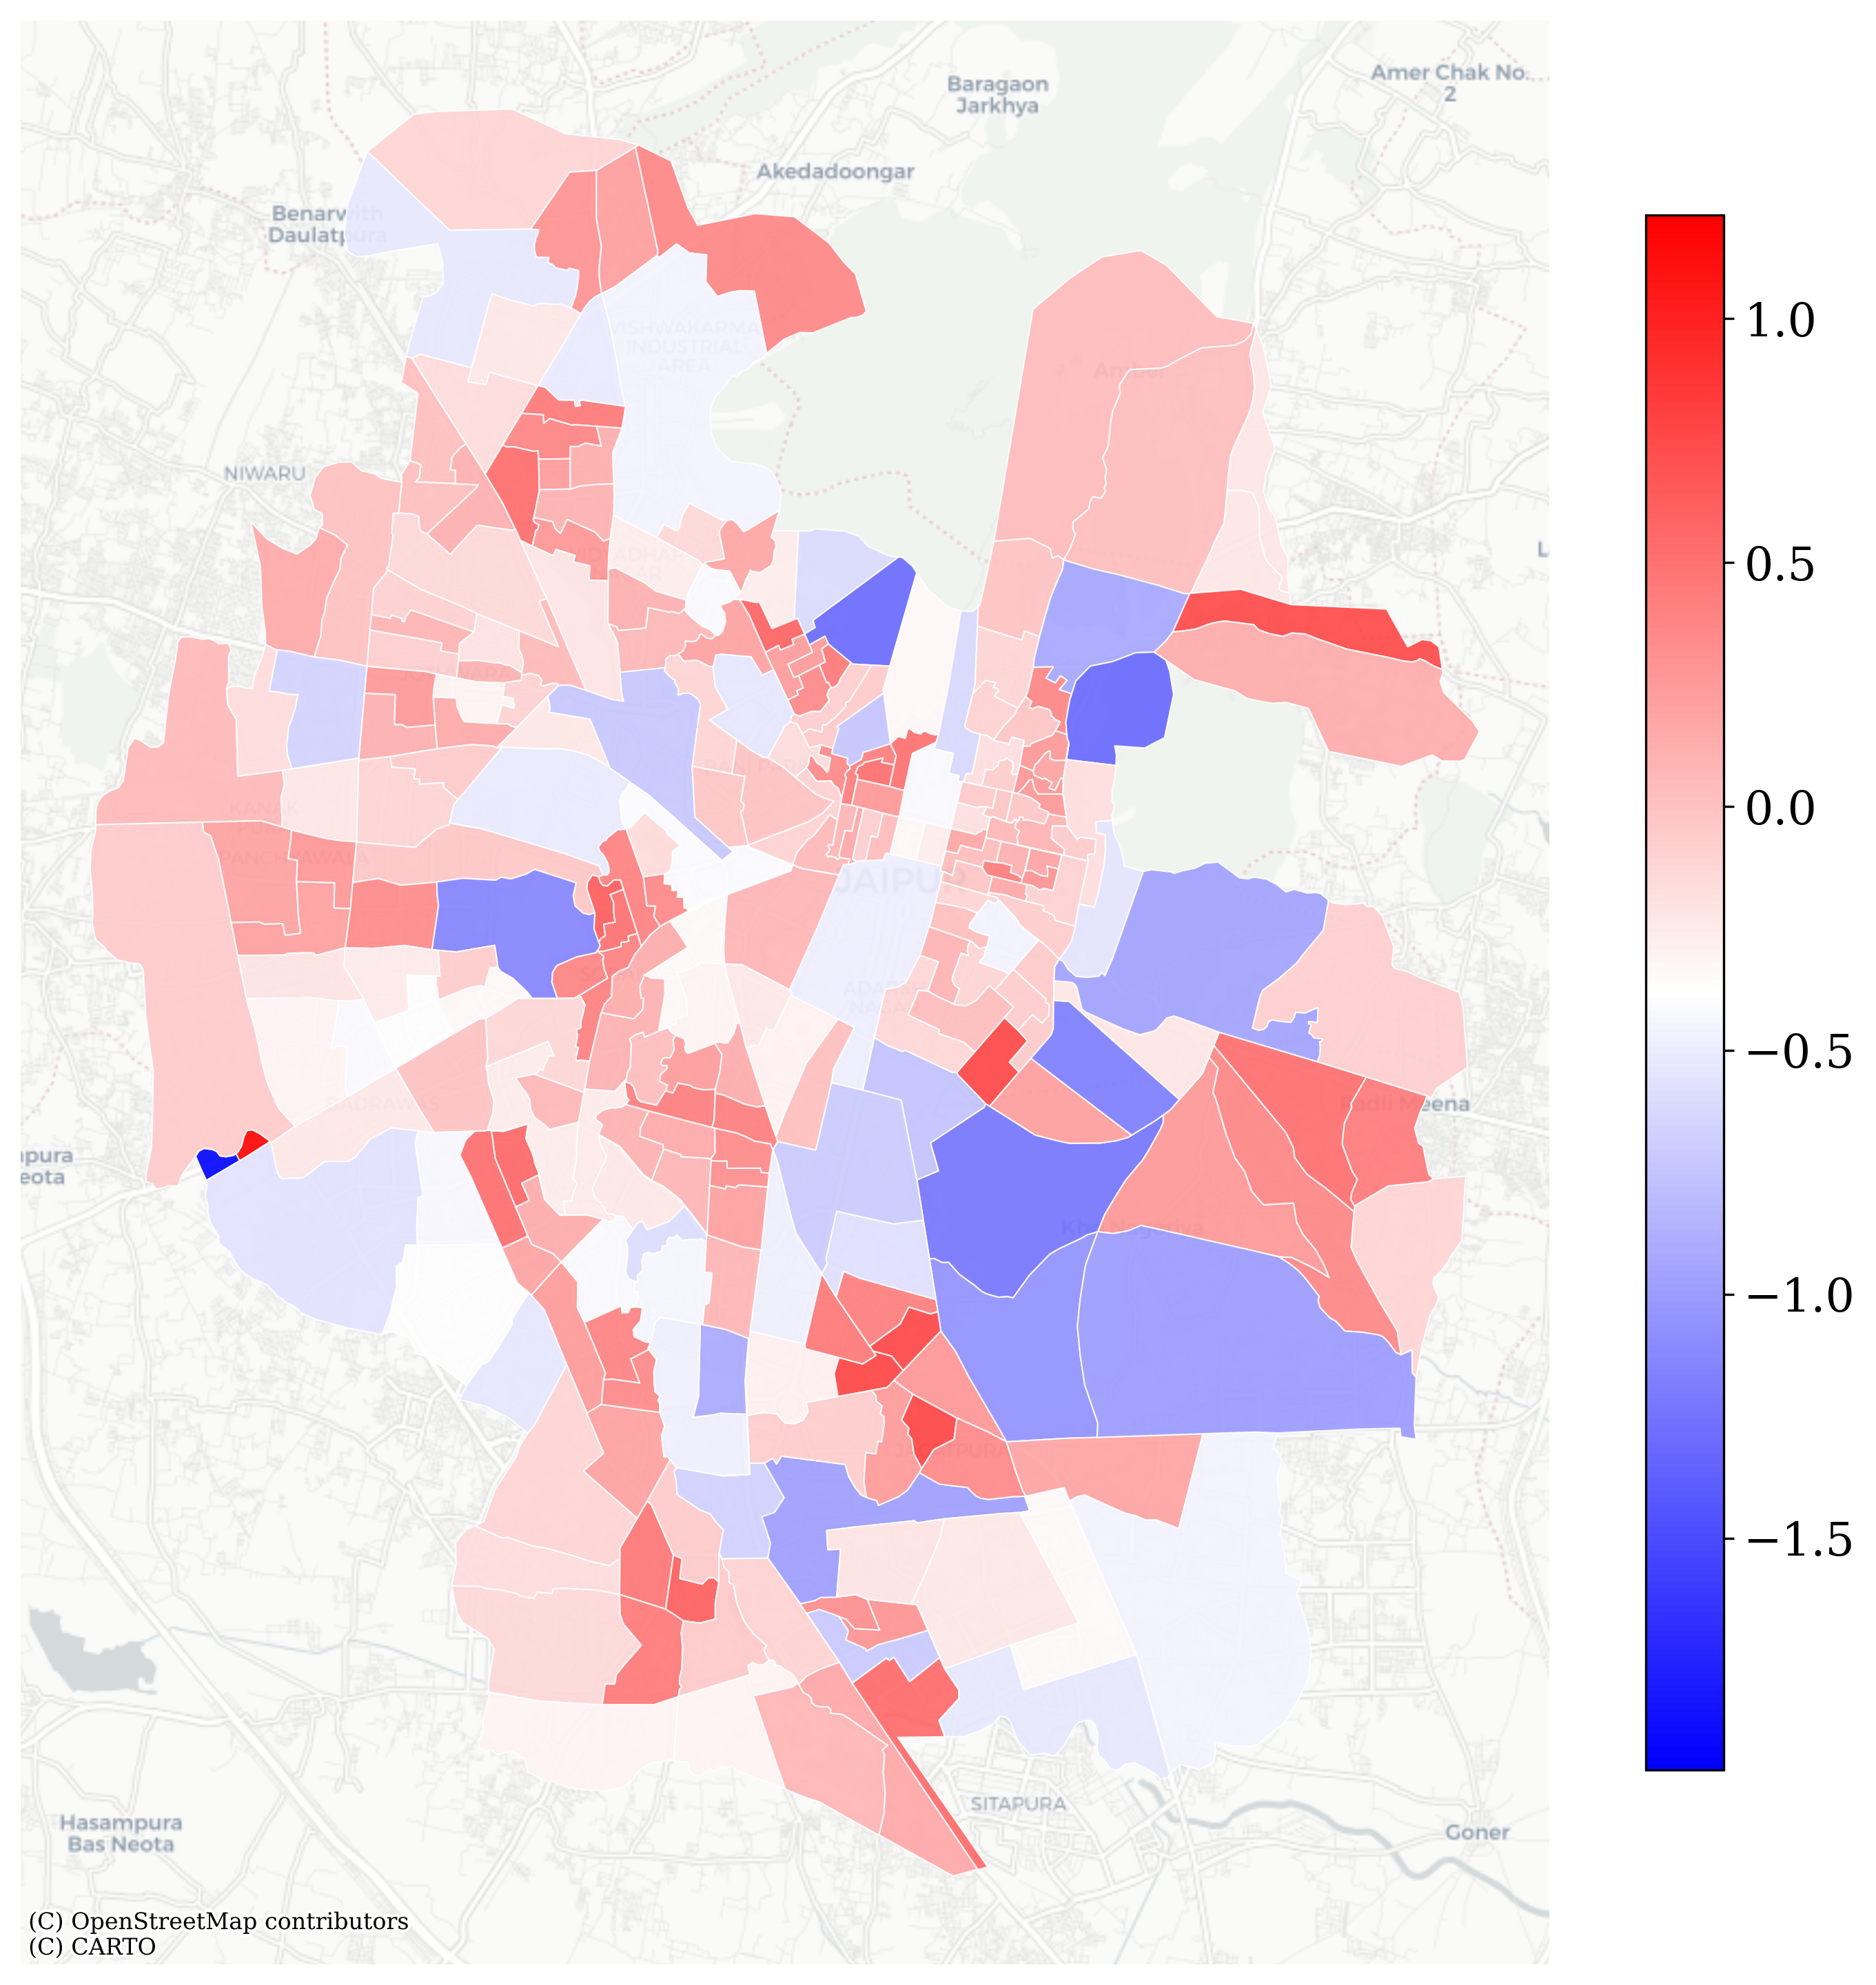
\includegraphics[width=0.6\linewidth]{thesis_images/04RE_residuals_map_gaussian_mgwr} 

}

\caption{MGWR Residuals Distribution Map}\label{fig:04RE-residual}
\end{figure}

\begin{figure}

{\centering \subfloat[Residual–fitted\label{fig:04RE-residual-diagnostics-1}]{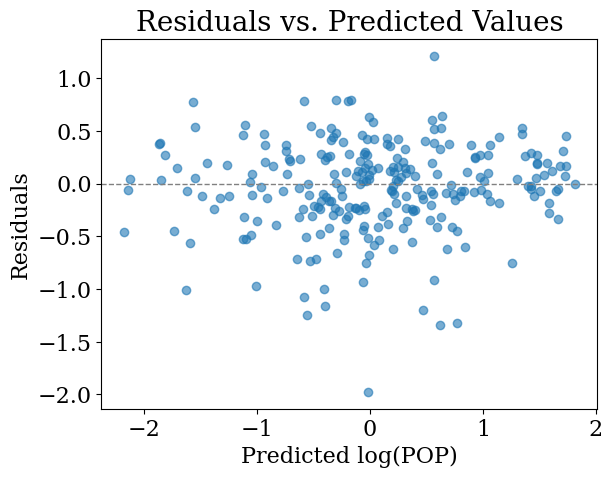
\includegraphics[width=0.49\linewidth]{thesis_images/04RE_residues} }\subfloat[Q–Q plot\label{fig:04RE-residual-diagnostics-2}]{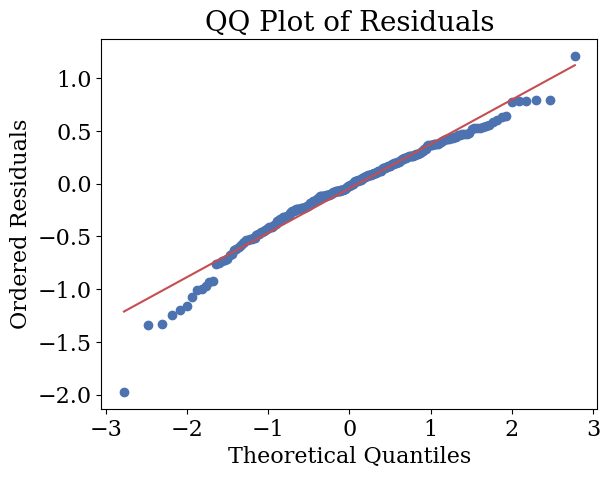
\includegraphics[width=0.49\linewidth]{thesis_images/04RE_qqplot} }

}

\caption{Residual Diagnostics: Residual–fitted and Q–Q plot}\label{fig:04RE-residual-diagnostics}
\end{figure}

\begin{figure}

{\centering 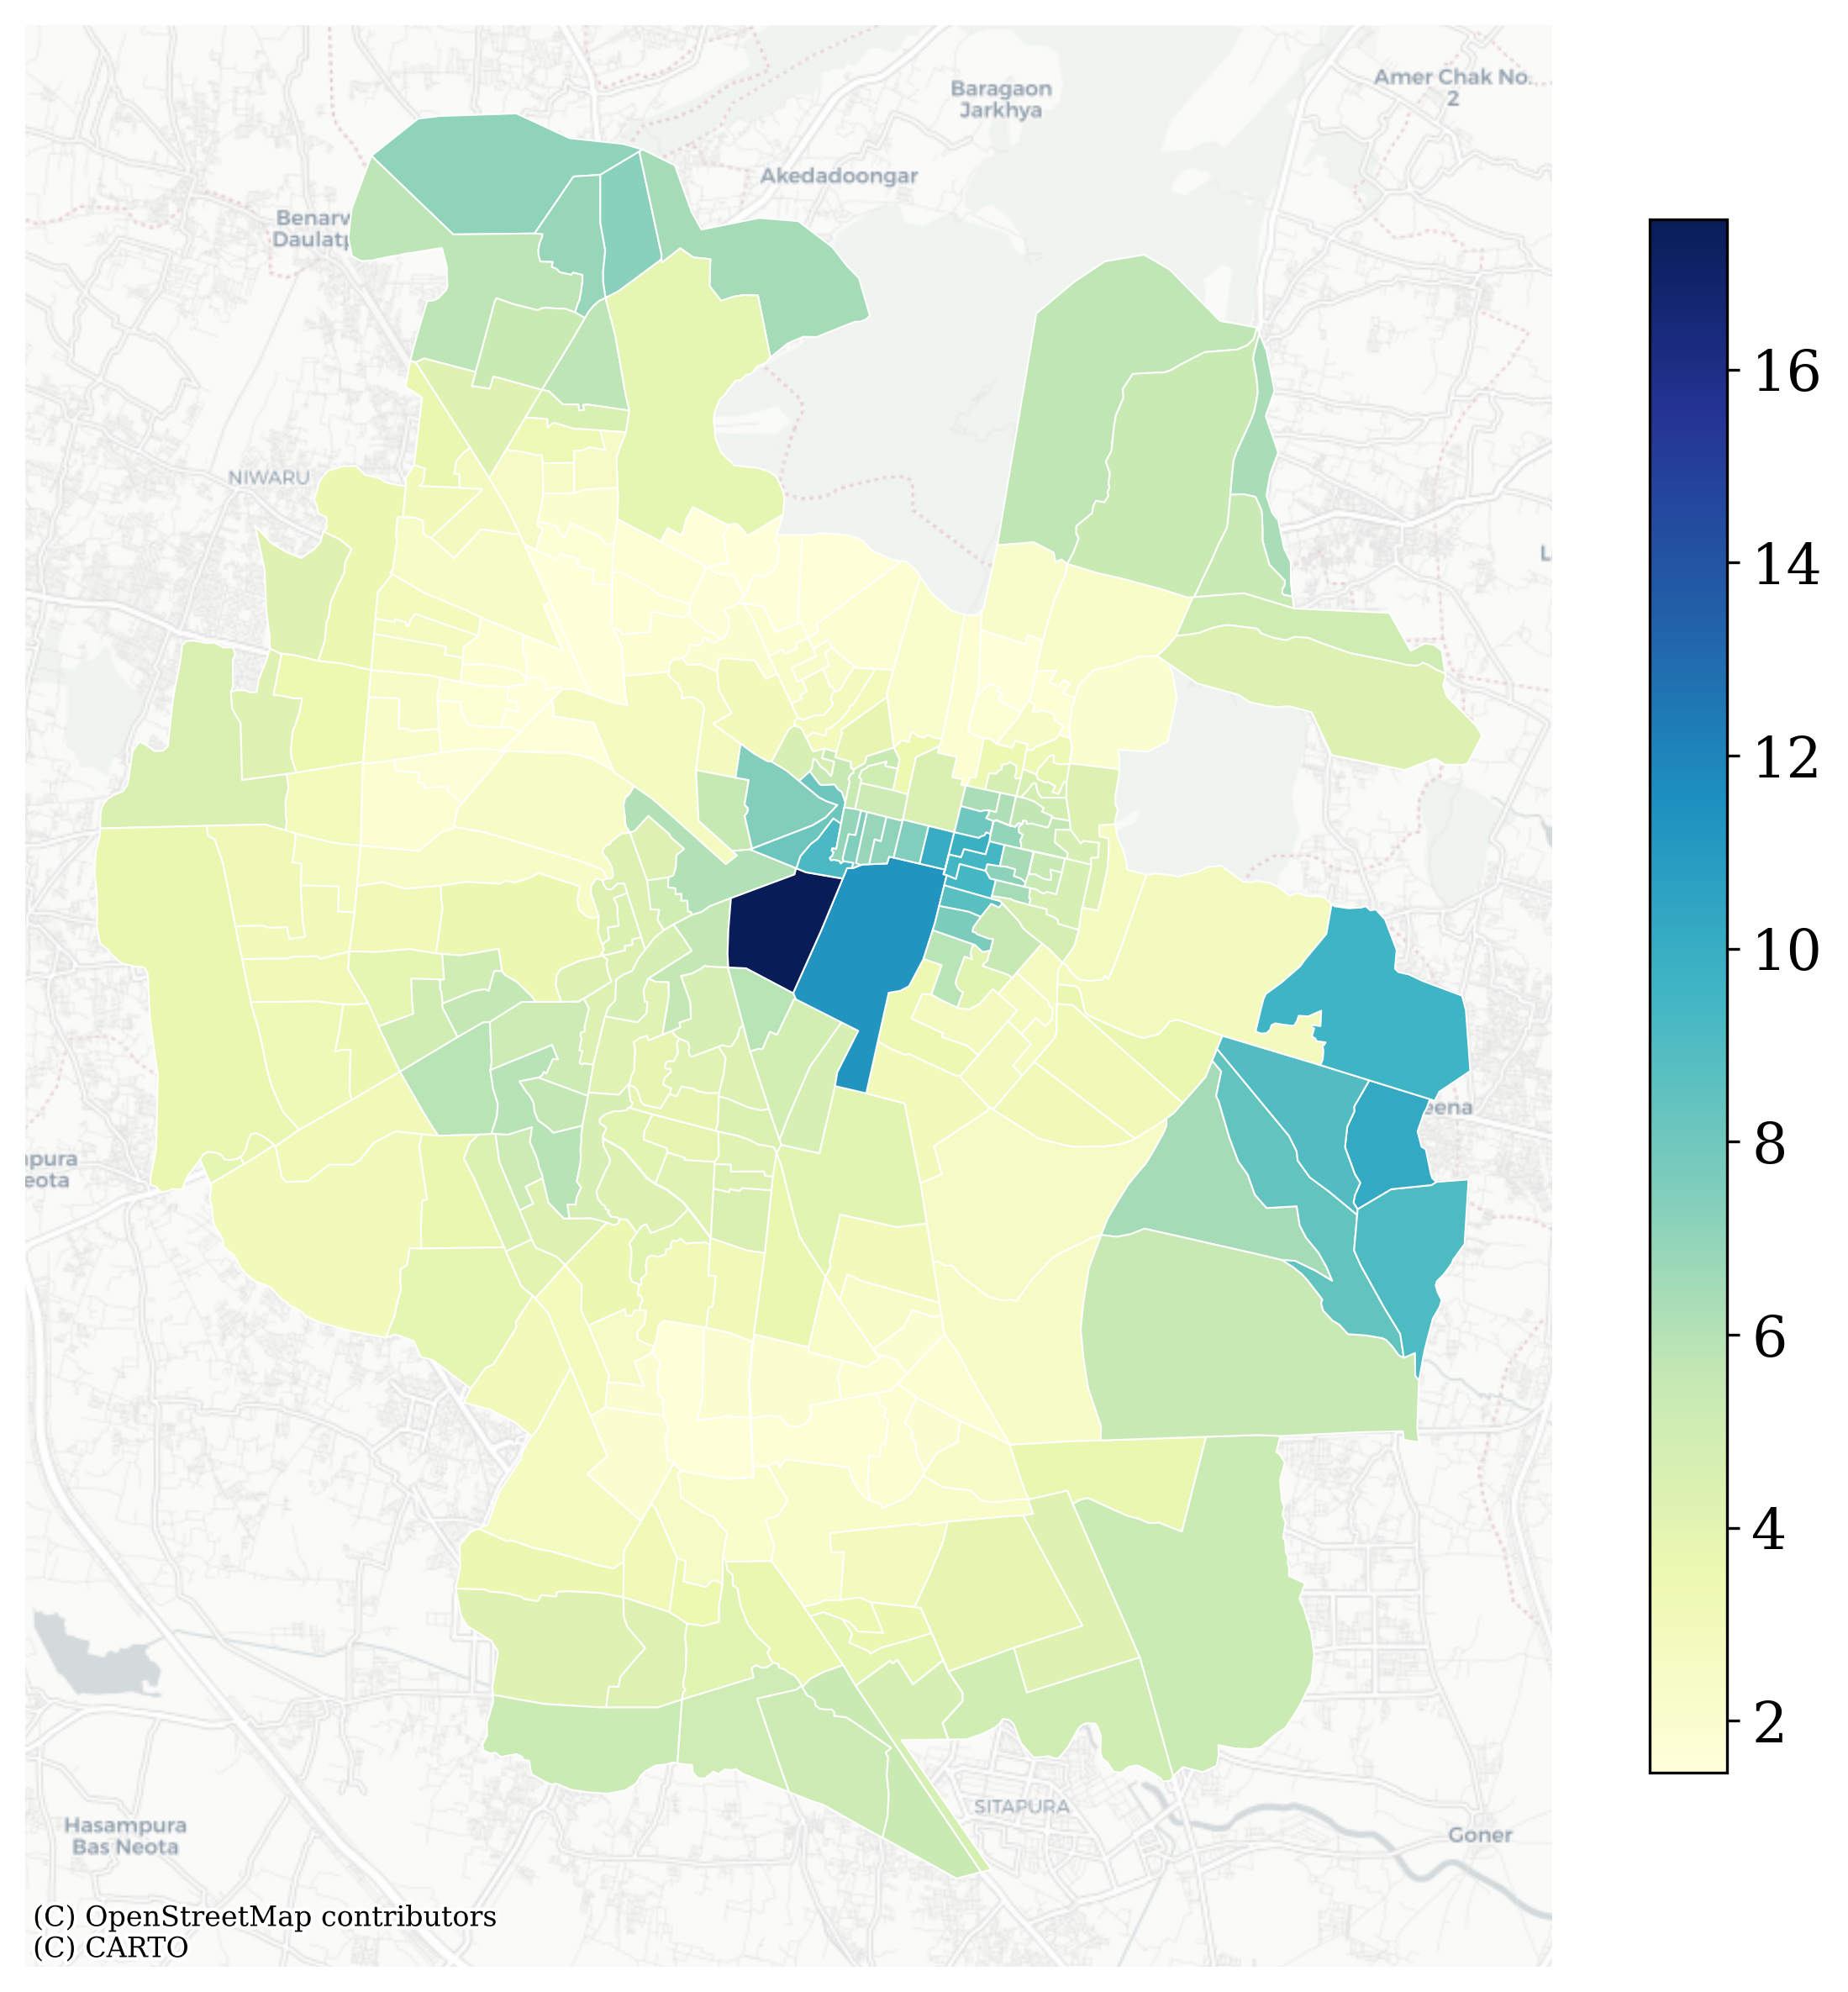
\includegraphics[width=0.6\linewidth]{thesis_images/04RE_CN_local_multicollinearity} 

}

\caption{MGWR Local Multicollinearity Test using Condition Number }\label{fig:04RE-CN}
\end{figure}

\subsection{Estimated Population Maps}\label{estimated-population-maps}

Figure \ref{fig:04RE-wardvsmgwr} compares the ward-level population distribution with the MGWR-derived 100 m raster estimates. While the ward-level map provides a broad overview, its reliance on administrative boundaries produces artificial discontinuities and conceals intra-ward heterogeneity.

Using weights estimated from the MGWR model, ward populations were disaggregated onto a 100 m grid. The resulting surface reveals finer spatial detail, with pronounced concentrations along Jaipur's central urban corridors and particularly dense clusters in the historic core. Secondary concentrations are also visible in the northwest and southeast, reflecting emerging population centres. Non-residential areas remain blank by design, reflecting the methodological assumption that only residential zones accommodate population.

The gridded representation offers a more nuanced view of settlement patterns by mitigating boundary effects and uncovering within-ward variation that coarse administrative data cannot capture.

\begin{figure}

{\centering 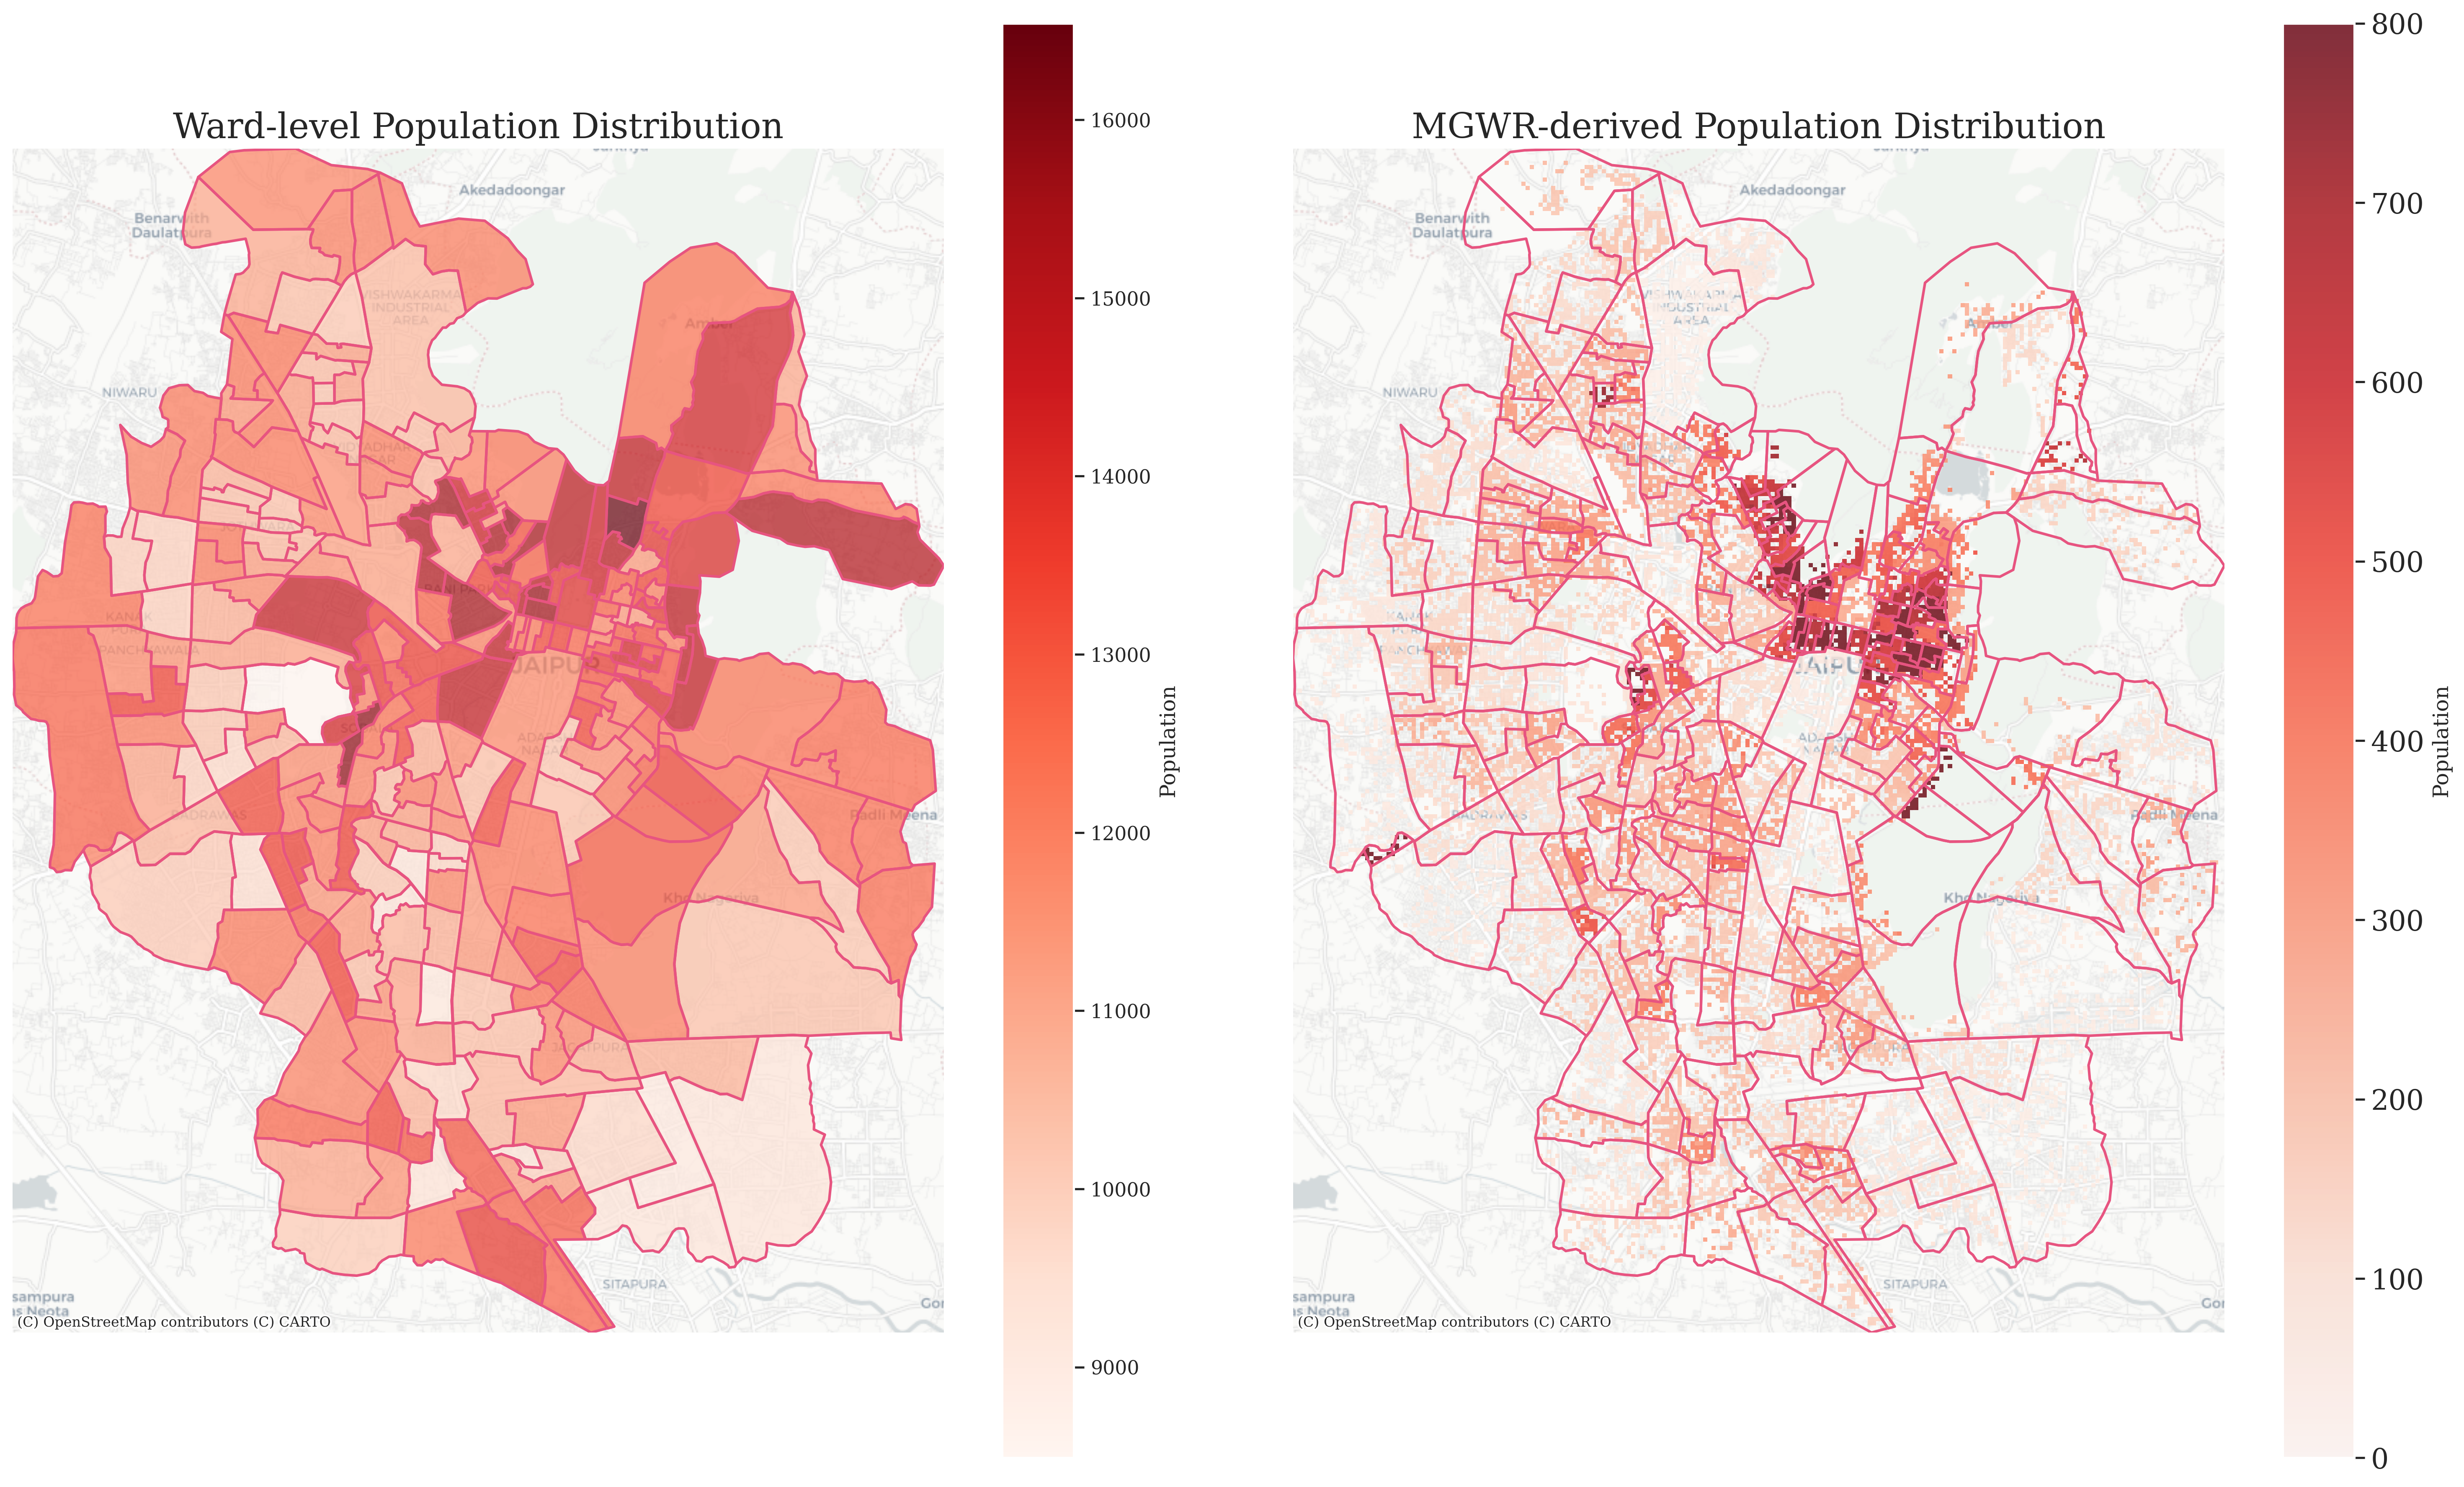
\includegraphics[width=0.98\linewidth]{thesis_images/04RE_wardvsmgwr} 

}

\caption{Ward-level Population Distribution vs MGWR-derived Population Distribution}\label{fig:04RE-wardvsmgwr}
\end{figure}

\subsection{Distribution Validation with GHSL}\label{distribution-validation-with-ghsl}

To assess the plausibility of the MGWR-based disaggregation, the resulting population grid was compared with the 2020 GHSL (GHS-POP) estimates for Jaipur. GHSL was selected as a reference because it applies a similar principle of allocating population only to residential built-up areas, ensuring a consistent basis for comparison \autocite{pesaresiAdvancesGlobalHuman2024a}.

Figure \ref{fig:04RE-GHSL-pop} shows the distribution of population counts per 100 m grid (equivalent to residents per hectare). Both datasets follow a broadly similar pattern: the majority of cells contain fewer than 200 residents per hectare, while a small number of high outliers capture the contrast between Jaipur's compact historic core and its more dispersed periphery.

\begin{figure}

{\centering 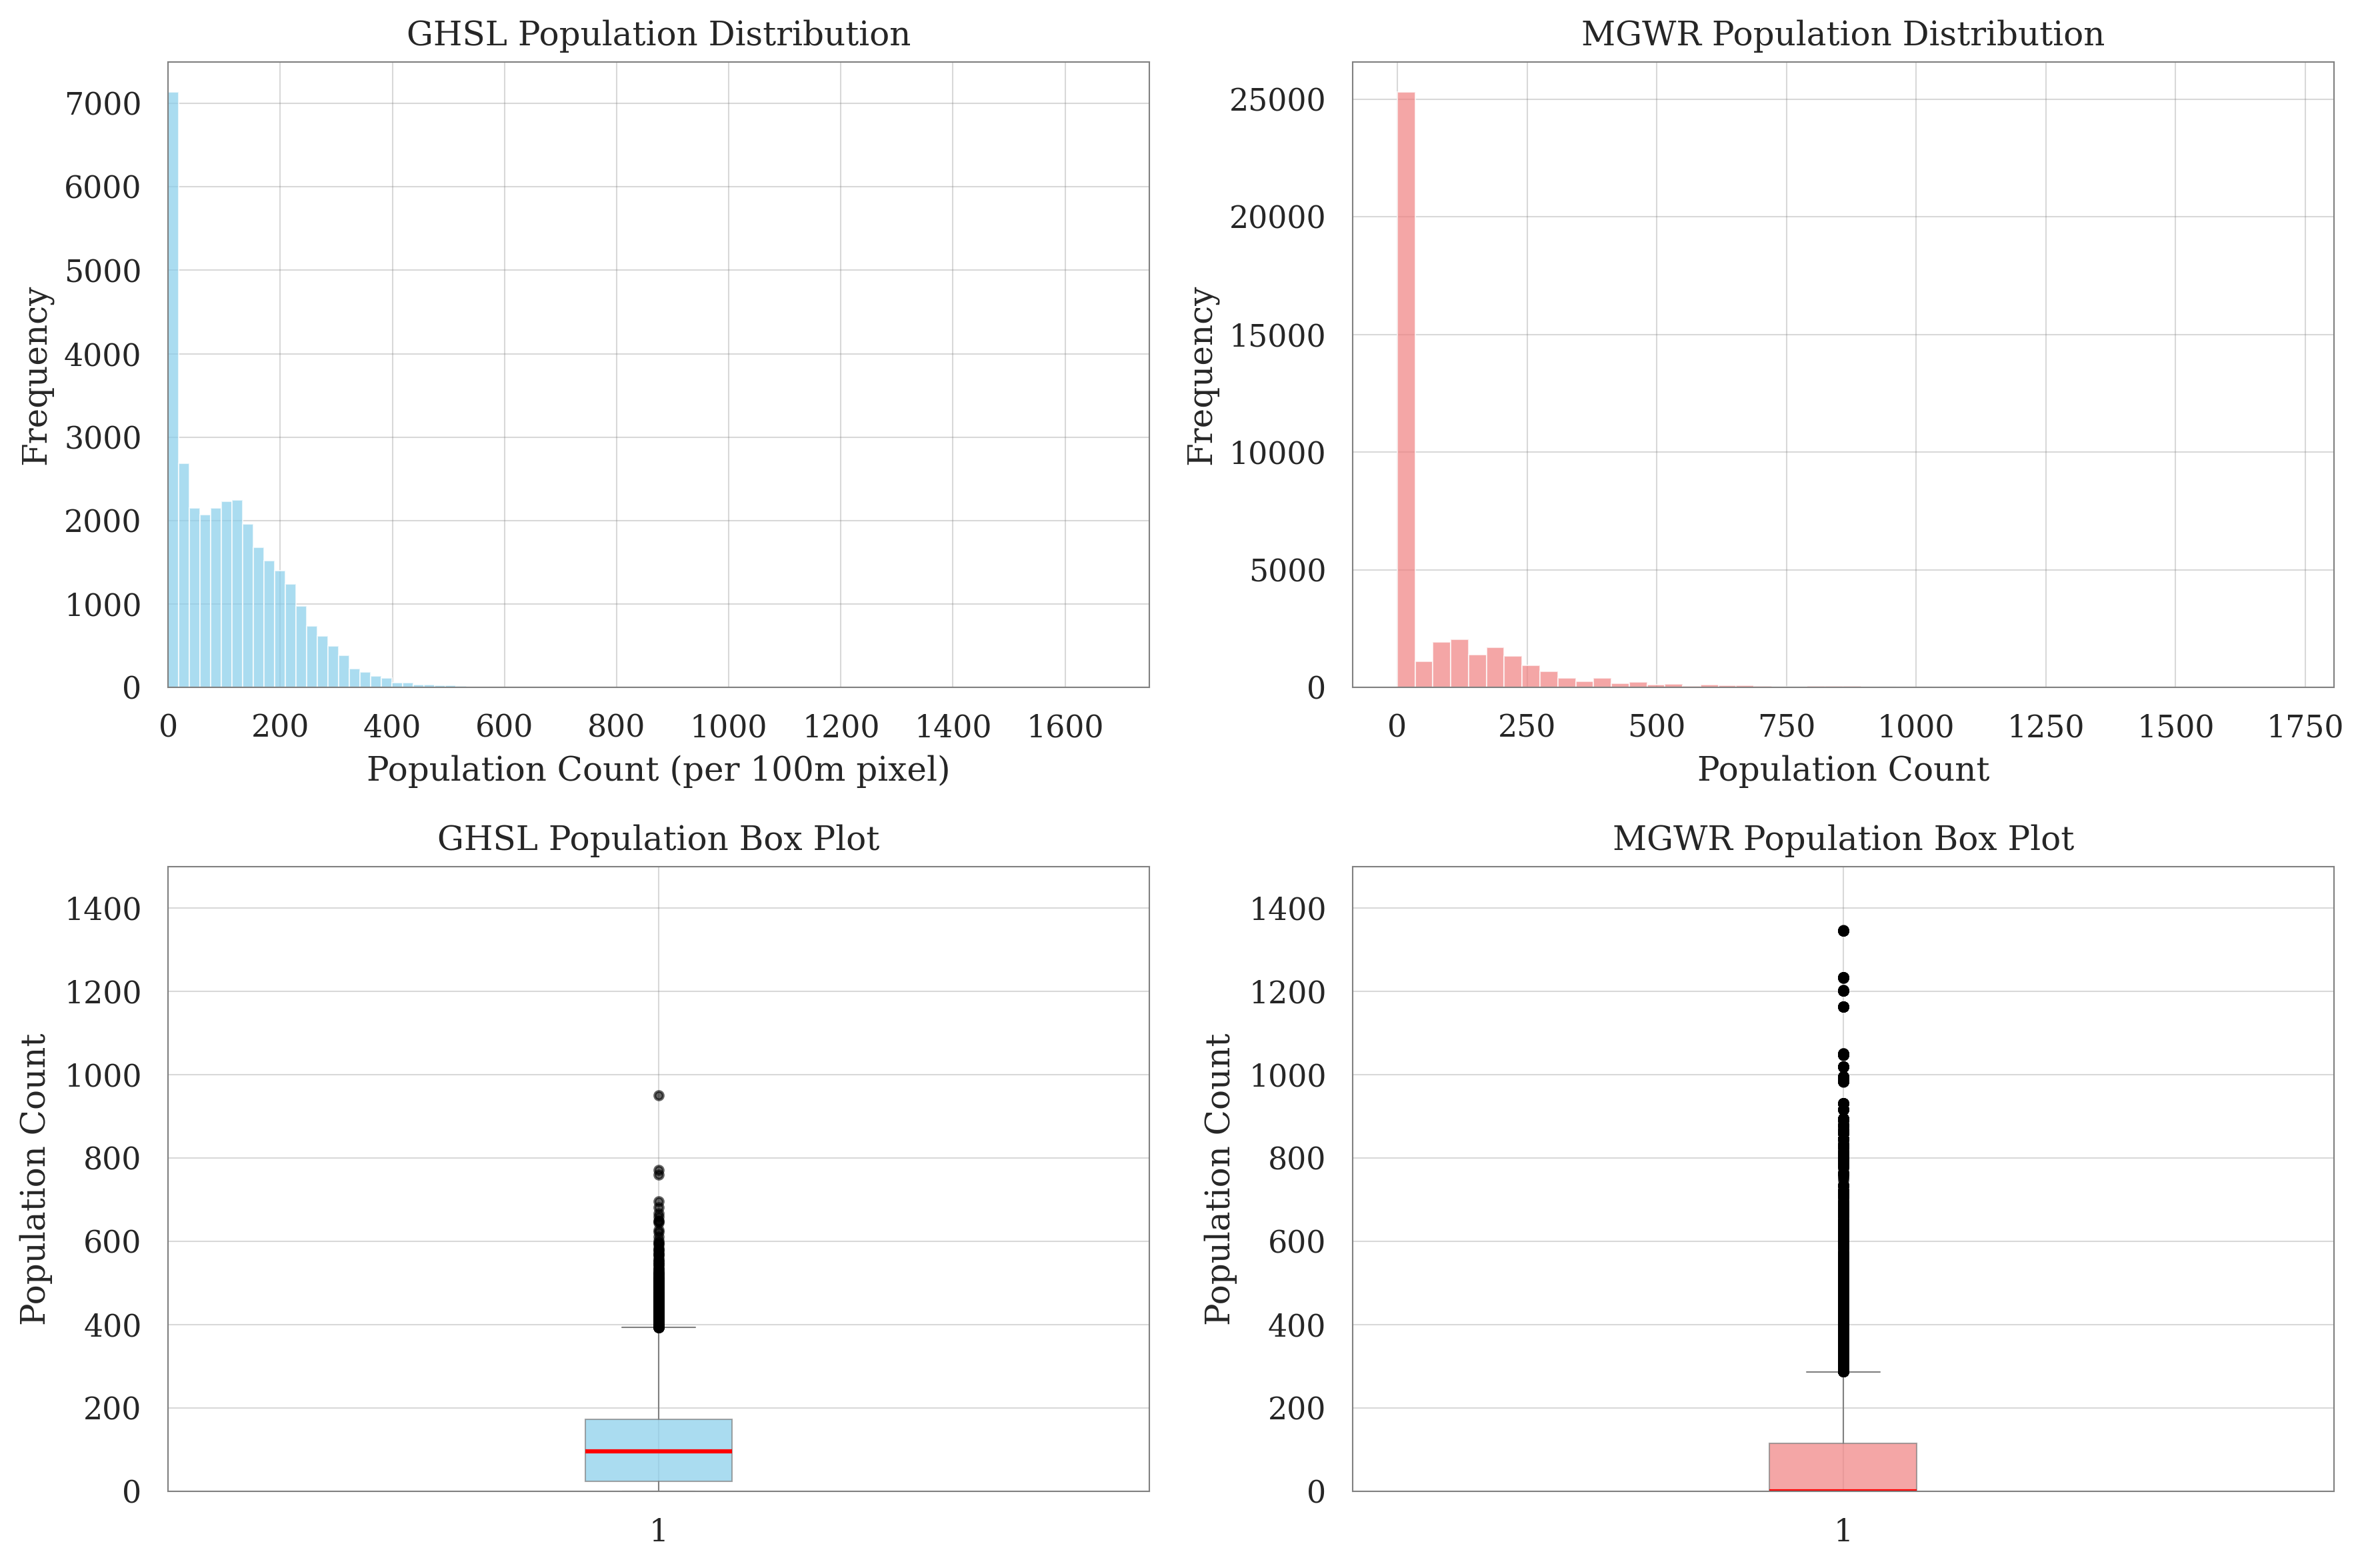
\includegraphics[width=0.98\linewidth]{thesis_images/04RE_GHSL_compare} 

}

\caption{GHSL vs MGWR Population Distribution (per hectare) }\label{fig:04RE-GHSL-pop}
\end{figure}

Notable differences also emerge. The MGWR estimates exhibit a sharper spike at very low values, which largely reflects cells excluded under the residential mask rather than genuinely low-populated areas. In contrast, GHSL produces a smoother distribution, with more cells assigned to the mid-density range (200--400). At the high end, MGWR shows a heavier tail, with a greater number of cells exceeding 1,000 residents per hectare.

Overall, the two datasets align in their general distributional shape, but MGWR produces a more polarised outcome---many empty or low-population cells alongside a concentration of very dense ones. This reflects the methodological choice to restrict disaggregation strictly to residential built-up areas using locally estimated weights, whereas GHSL relies on a global building-volume proxy that spreads population more evenly. The latter approach allows consistent disaggregation worldwide, but it also has limitations: uniform global rules may overlook local land-use distinctions, accuracy depends on the resolution of built-up inputs, and recent changes---especially in rapidly growing or informal settlements---may be underrepresented. For these reasons, GHSL provides a useful benchmark for comparison, but should not be regarded as ground truth at the local scale.

\subsection{Explanatory Variables Shaping Population Density in the MGWR}\label{explanatory-variables-shaping-population-density-in-the-mgwr}

The MGWR results indicate that explanatory variables influence population density at different spatial scales. The intercept and light intensity operate at a local scale (bandwidth = 43 wards), POI kernel density at a regional scale (98 wards), and illuminated building volume density at a global scale (227 wards). This range demonstrates that population patterns are shaped simultaneously by neighbourhood-level dynamics and broader structural forces.

The spatial distribution of coefficients further underscores these heterogeneous effects (Figure \ref{fig:04RE-MGWR-coeff}):

\begin{itemize}
\item
  \textbf{Illuminated Building Volume Density (Global, BW = 227):} Coefficients are consistently negative across the city (mean = −0.516, range = −0.544 to −0.483, SD = 0.013). Large contiguous areas remain significant after correction, revealing a robust and spatially stable inverse relationship: higher illuminated volumes are systematically associated with lower population density. Significant clusters are most apparent in northern and western wards, as well as some peripheral zones.
\item
  \textbf{Nighttime Lights Intensity (Local, BW = 43):} Coefficients vary in direction (mean = 0.298, range = −0.238 to 1.054, SD = 0.273), with positive patches in eastern and peripheral areas and negative values in parts of the centre. Only small pockets remain significant after correction, reflecting a highly localized and heterogeneous effect.
\item
  \textbf{POI Kernel Density (Regional, BW = 98):} Coefficients are generally positive (mean = 0.192, range = 0.061 to 0.545, SD = 0.144). Strong effects are concentrated along the southern and eastern corridors, where dense POI clusters coincide with higher residential density. Central wards and parts of the periphery show non-significant values, highlighting the uneven influence of POI kernel density.
\item
  \textbf{Intercept (Local, BW = 43):} Local intercepts vary from negative to positive (mean = 0.230, range = −0.357 to 0.771, SD = 0.322). Significant estimates cluster around the city core and isolated edge wards, indicating baseline differences in population density not captured by the current covariates.
\end{itemize}

\begin{figure}

{\centering 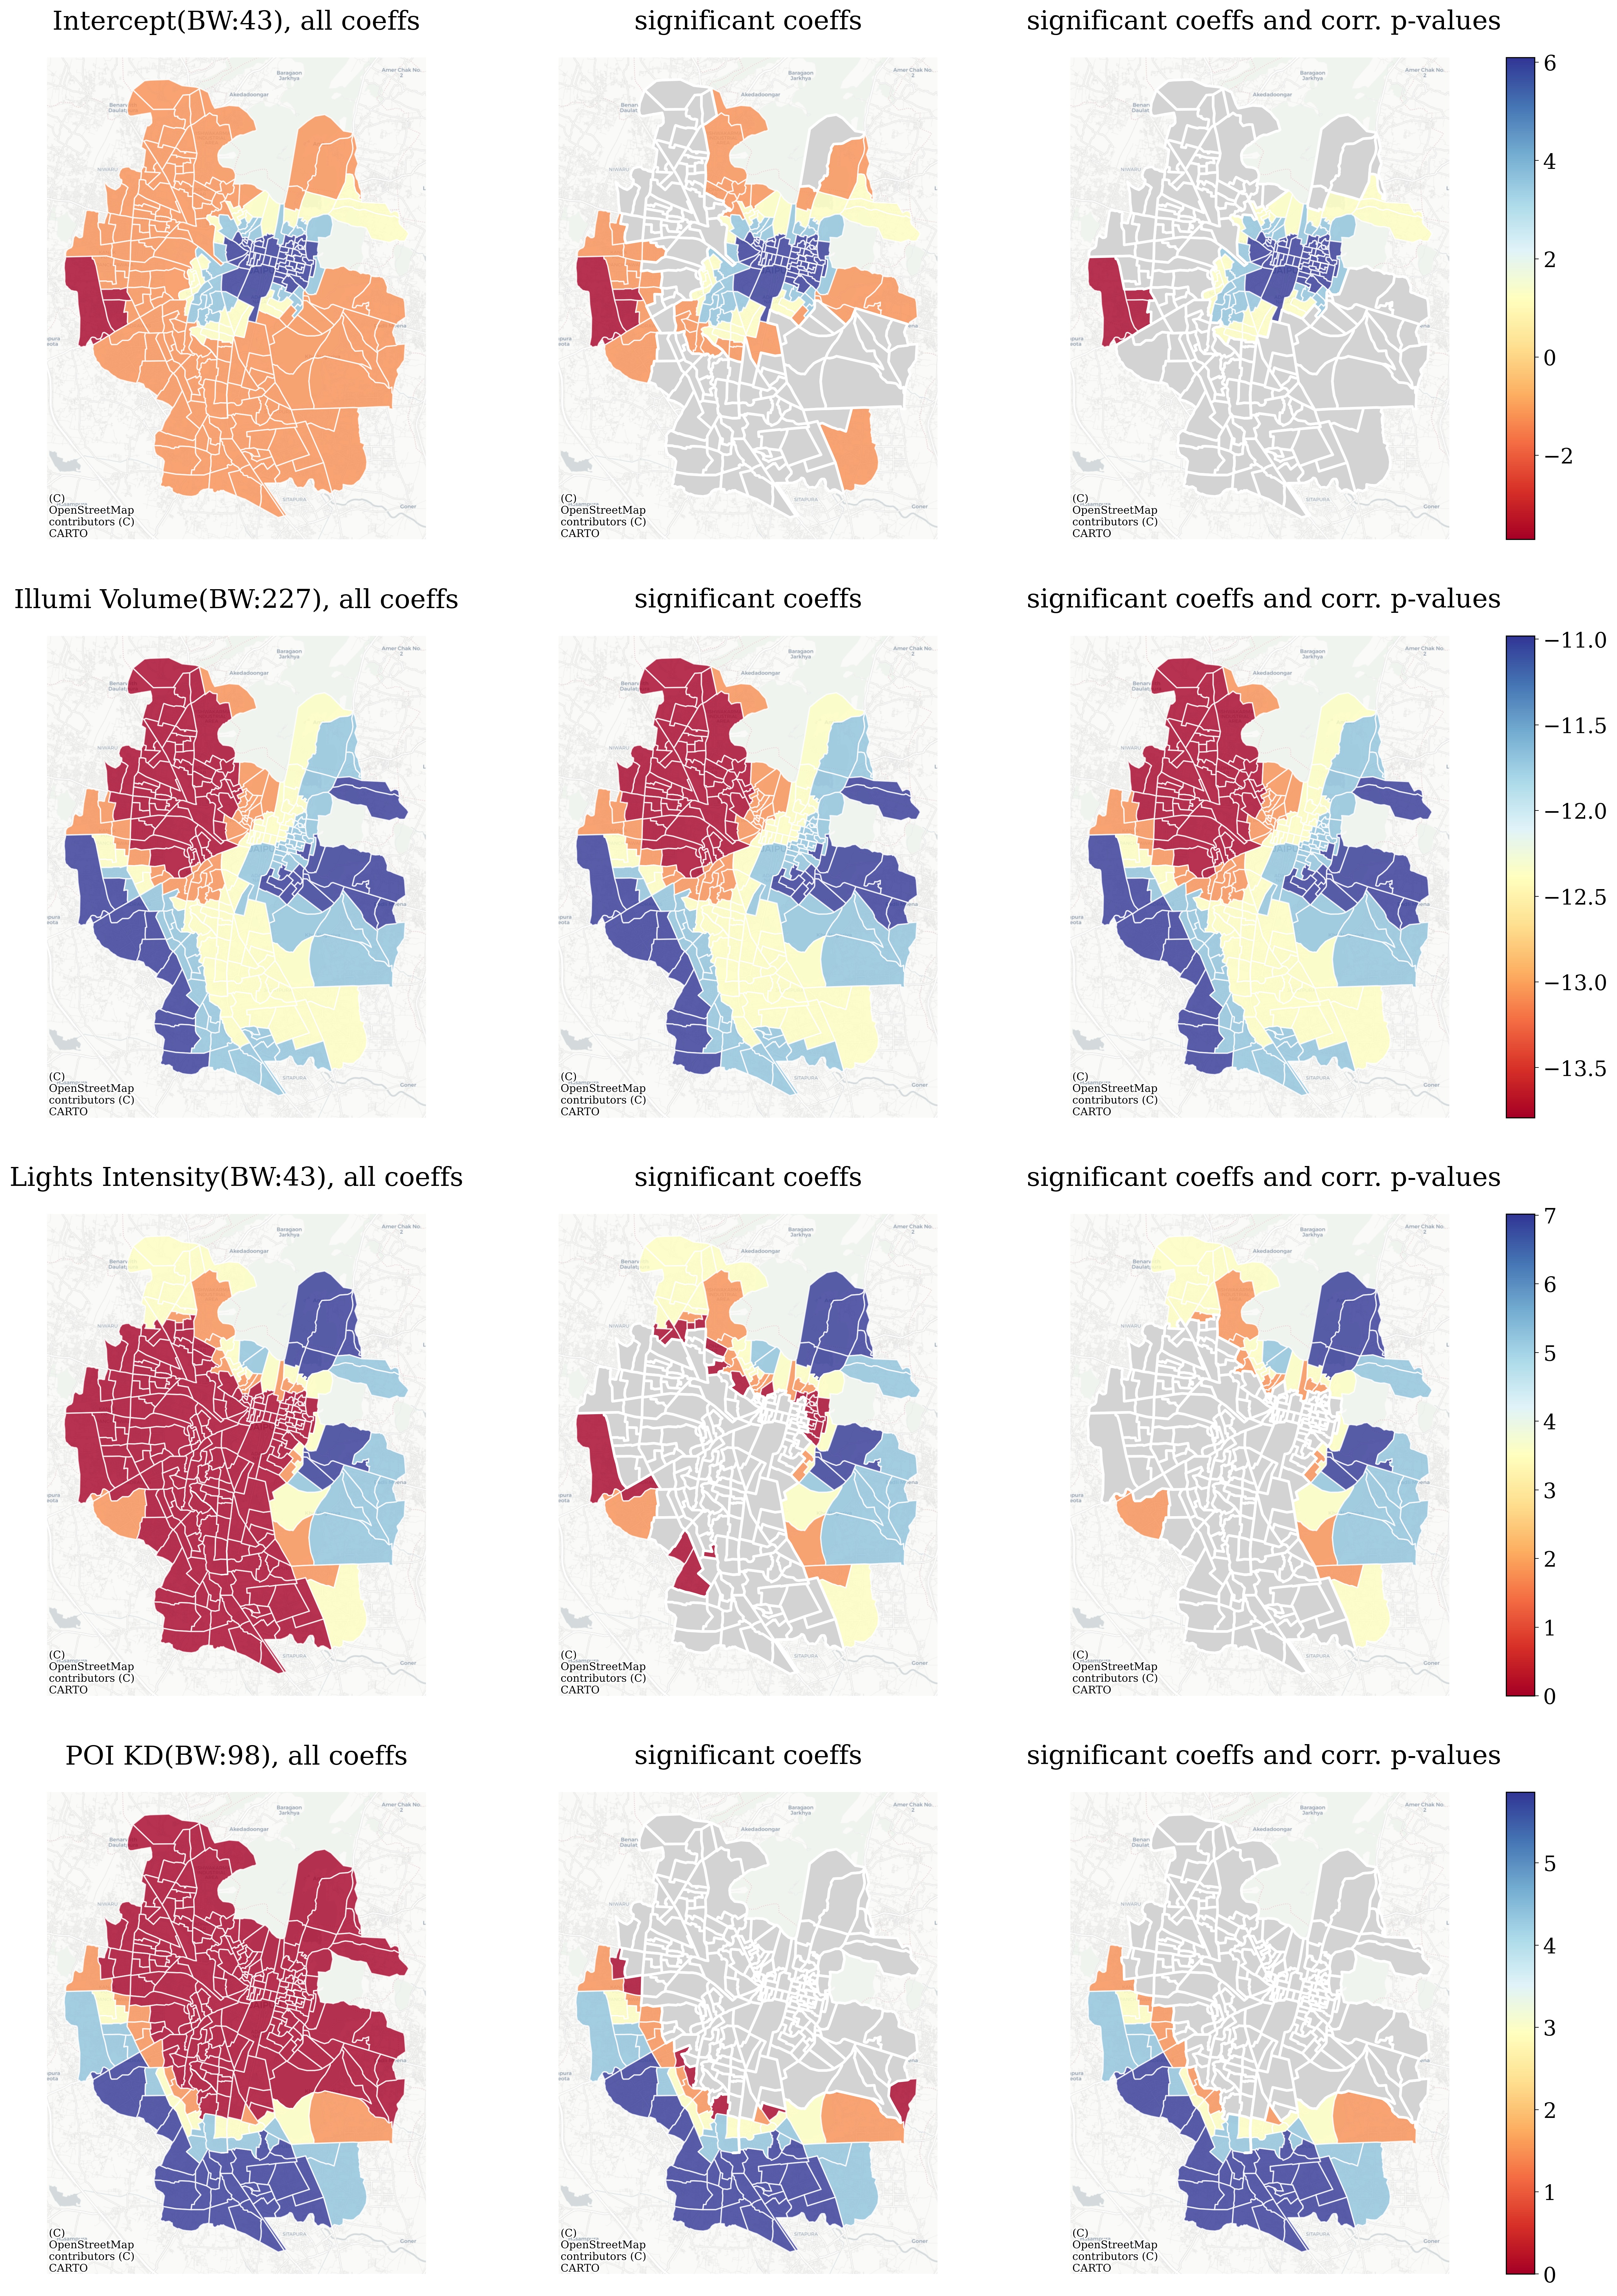
\includegraphics[width=0.9\linewidth]{thesis_images/04RE_mgwr_all_significant_coeffs} 

}

\caption{Coefficients Estimates for Explanatory Variables in the MGWR model: illuminated building volume density, nighttime lights intensity, POI kernel density and intercept. For each variable, the left panel shows raw parameter estimates, the middle panel displays significant and non-significant estimates without correction (non-significant in grey), and the right panel presents estimates after correction for multiple dependent hypothesis tests, where only statistically significant coefficients remain colored (red = negative, blue = positive).}\label{fig:04RE-MGWR-coeff}
\end{figure}

Key findings:

\begin{itemize}
\tightlist
\item
  Direction: Illuminated building volume density exerts a consistent negative effect, while POI kernel density shows a strong positive effect. Light intensity and the intercept display more fragmented influences.
\item
  Scale: Explanatory factors operate across levels, from local (intercept, light intensity) to regional (POI kernel density) and global (illuminated volume).
\item
  Significance: Illuminated volume shows the most robust and widespread effect, followed by POI kernel density; light intensity and the intercept are significant only in scattered clusters.
\end{itemize}

To sum up, the MGWR results demonstrate that population density in Jaipur is driven by both heterogeneous directions and multi-scale processes. The model highlights robust citywide effects of illuminated building volume, regionally concentrated influence of POI kernel density, and more localized variations linked to light intensity and intercept terms. This underlines the value of a multi-scale approach for decomposing urban population patterns.

\section{Response to RQ1: Where Economic Activity levels are High -- Economic Activity Index (EAI)}\label{response-to-rq1-where-economic-activity-levels-are-high-economic-activity-index-eai}

\subsection{Correlation among Input Variables}\label{correlation-among-input-variables}

Before conducting PCA, the correlations among the ten selected indicators aggregated to 500 m hexagon cells were examined. Figure \ref{fig:04RE-pca-matrix} presents the correlation matrix.

The results show that population density, built-up density, road density, and nighttime lights are strongly and positively correlated (\(r \approx 0.6–0.8\)), indicating that they capture overlapping dimensions of urban development intensity and economic activity. In contrast, NDVI is strongly and negatively correlated with these variables, reflecting the trade-off between vegetation cover and built-up intensity. Large transport stations (e.g.~airports) display only weak negative correlations with activity-related indicators, consistent with their distinct spatial separation from daily economic clusters.

These correlations indicate substantial shared variation, justifying PCA to condense them into latent dimensions while retaining contrasting signals (e.g.~NDVI, transport stations) that help differentiate patterns.

\begin{figure}

{\centering 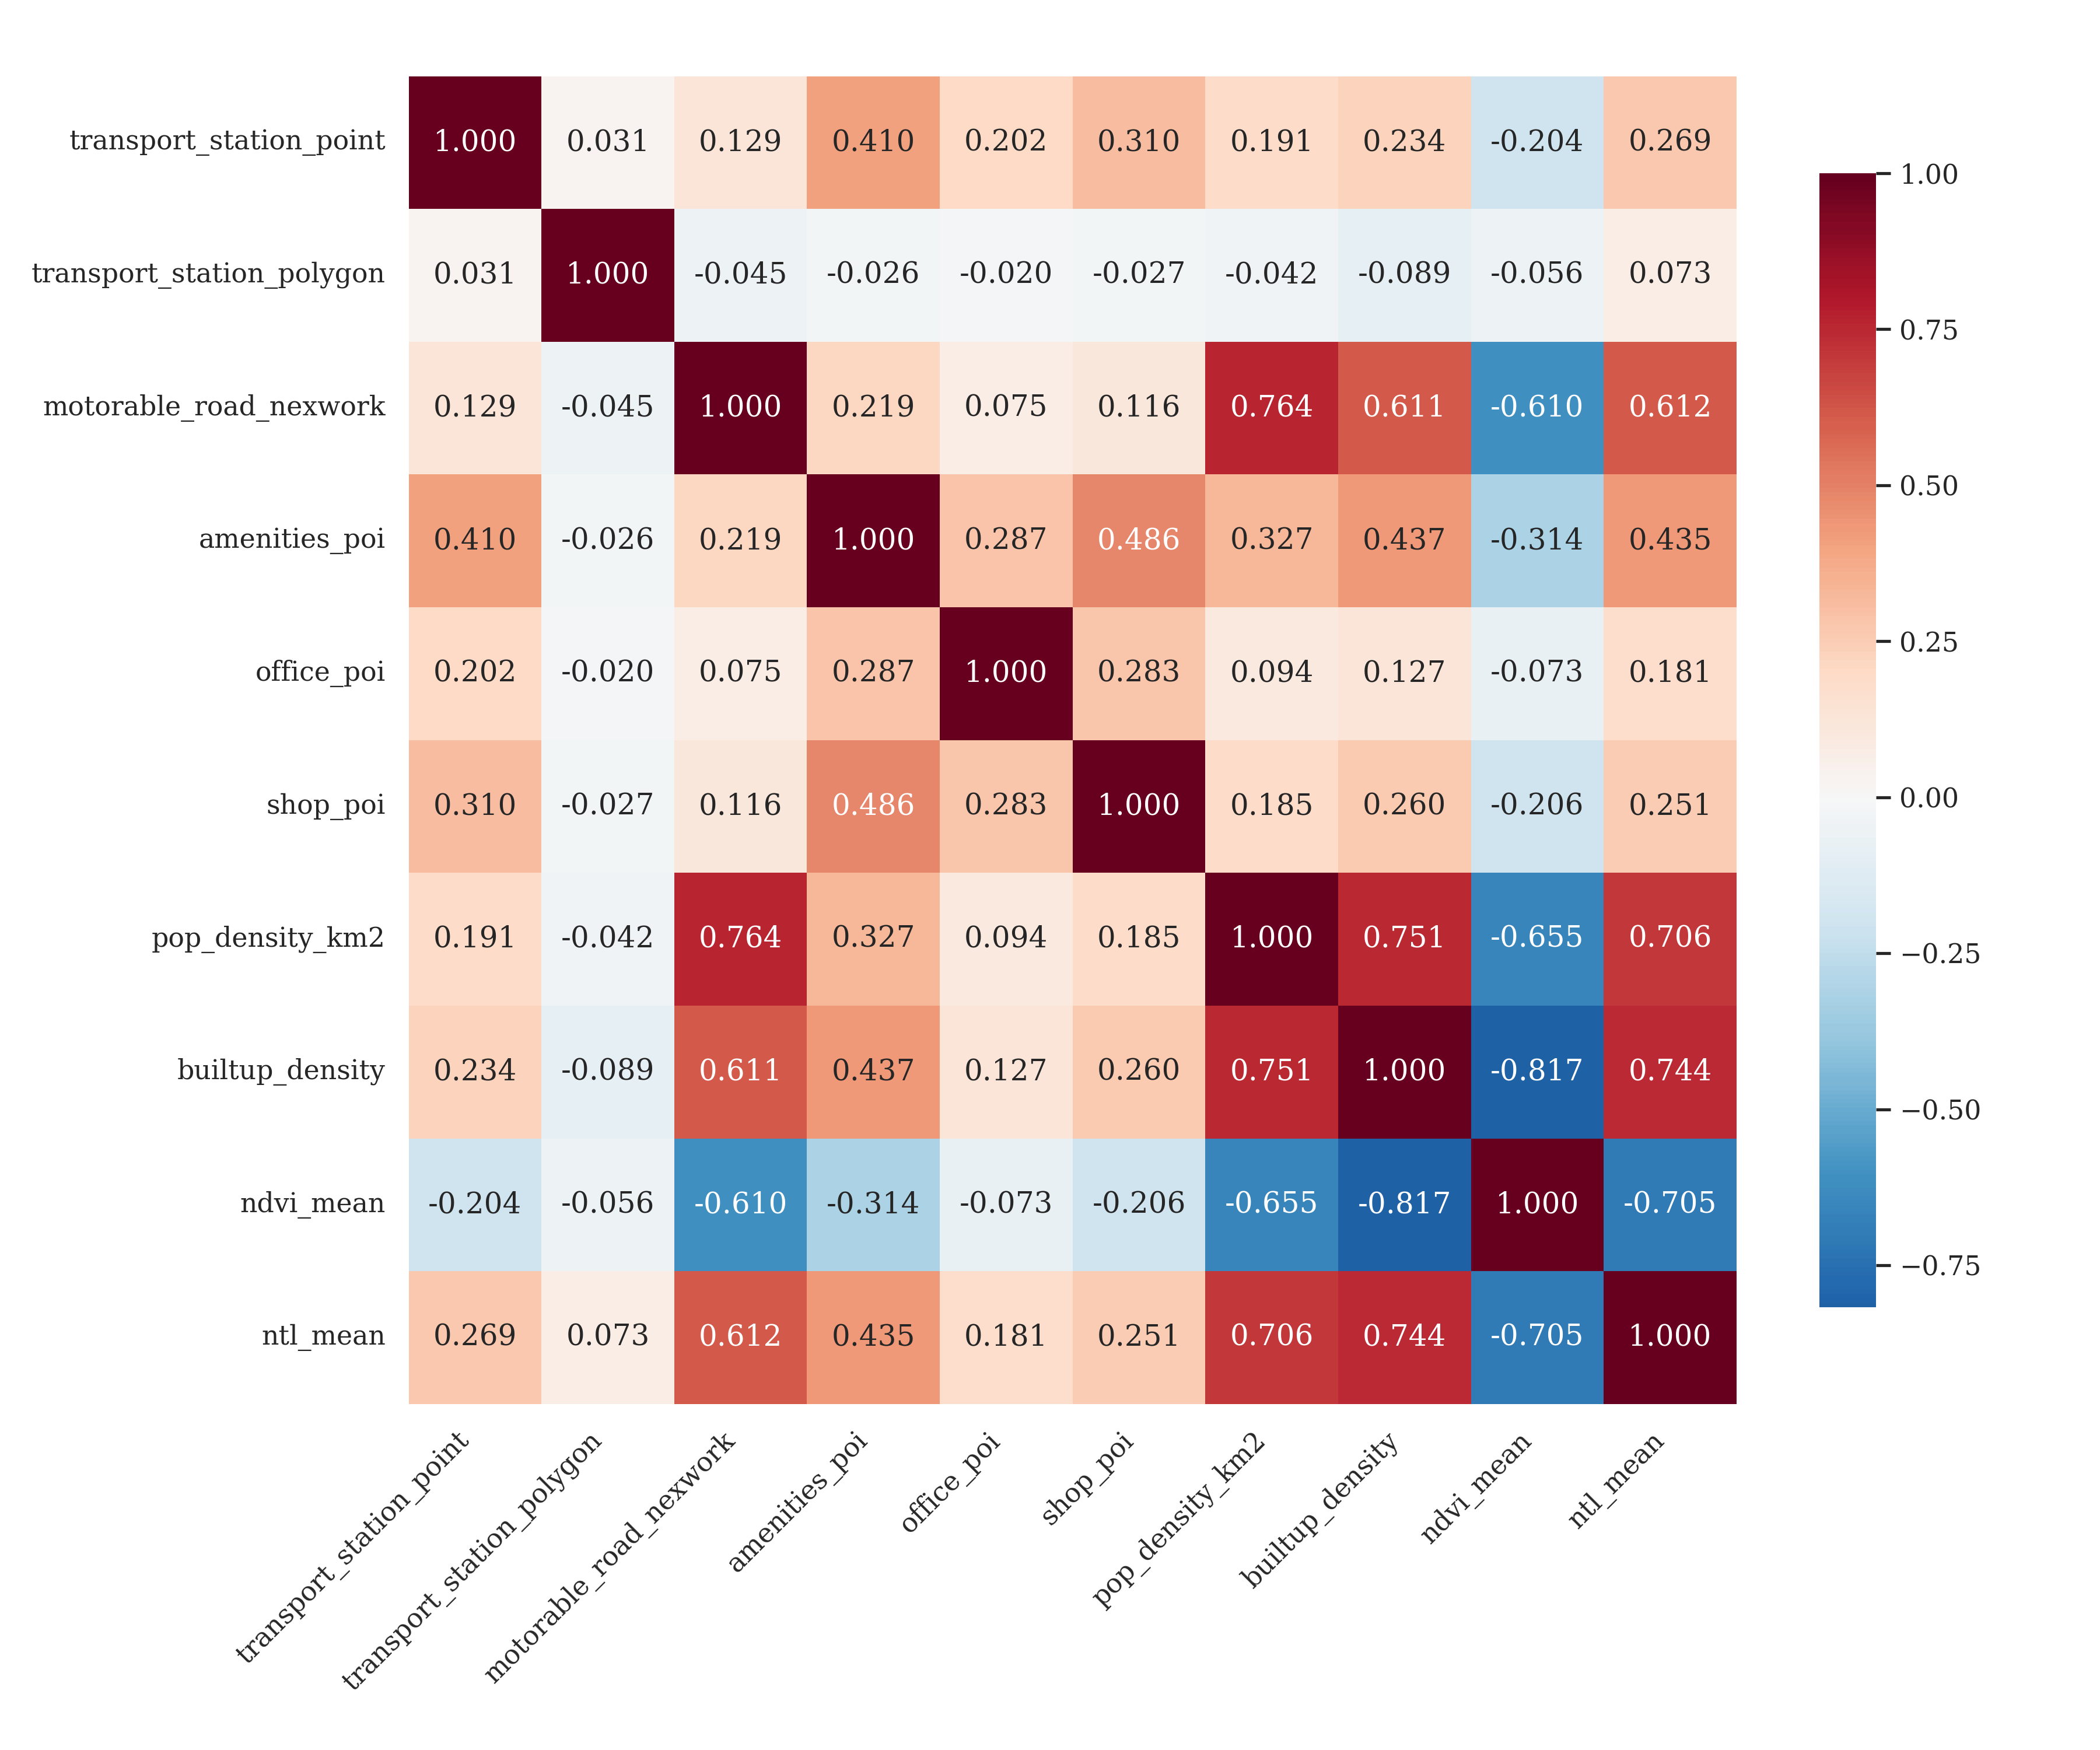
\includegraphics[width=0.98\linewidth]{thesis_images/04RE_correlation_heatmap_full_log_data} 

}

\caption{ PCA Variables Correlation Matrix }\label{fig:04RE-pca-matrix}
\end{figure}

\subsection{PCA Results}\label{pca-results}

The PCA results show that the first two components capture most of the shared variance among the indicators. The scree plot (Figure \ref{fig:04RE-pca-scree}) indicates a sharp drop after the first component, with eigenvalues of 4.3 for PC1 and 1.6 for PC2, together explaining 58.7\% of the total variance. This justifies focusing on PC1 and PC2 for interpretation and mapping.

The loadings (Table \ref{tab:pca-loadings}) highlight distinct roles of the indicators. PC1 (42.7\% of variance) is shaped by strong positive contributions from population density, built-up density, road density, POI, and nighttime lights, with NDVI and large transport polygons contributing negatively. In practical terms, PC1 can be interpreted as a dimension of economic activity intensity: hexagons scoring highly are characterised by dense built-up form, higher population and road density, many POI, and bright nighttime lights, combined with low vegetation cover and little presence of large transport infrastructure. This configuration corresponds closely to the empirical notion of concentrated urban economic activity. Therefore, PC1 will be chosen to construct the Economic Activity Index (EAI).

PC2 (16.0\% of variance) reflects a secondary dimension. It contrasts transport station points and office/shop POI against NDVI and large transport polygons, suggesting that this component differentiates localised commercial clusters from greener or large-scale infrastructural areas. In practice, PC2 highlights variations in the type of economic built environment, rather than the direct economic intensity.

The biplot (Figure \ref{fig:04RE-pca-biplot}) reinforces these relationships, showing built-up, population, road, and NTL vectors aligned, while NDVI and large transport polygons point in the opposite direction. Rather than isolated pairwise correlations, this configuration shows how PCA integrates divergent spatial signals---ranging from urban development and everyday POI density to green space and infrastructural scale---into interpretable components. These components reveal latent dimensions that organize Jaipur's economic geography, offering a structured lens on urban heterogeneity.

Thus, the PCA enables a meaningful reduction in dimensionality, distilling complex spatial-economic patterns into interpretable components. PC1 captures the primary axis of economic activity intensity, while PC2 reflects a secondary contrast in urban morphology. Together, these two components provide the foundation for constructing the EAI and guiding subsequent cluster analysis.

\begin{figure}

{\centering 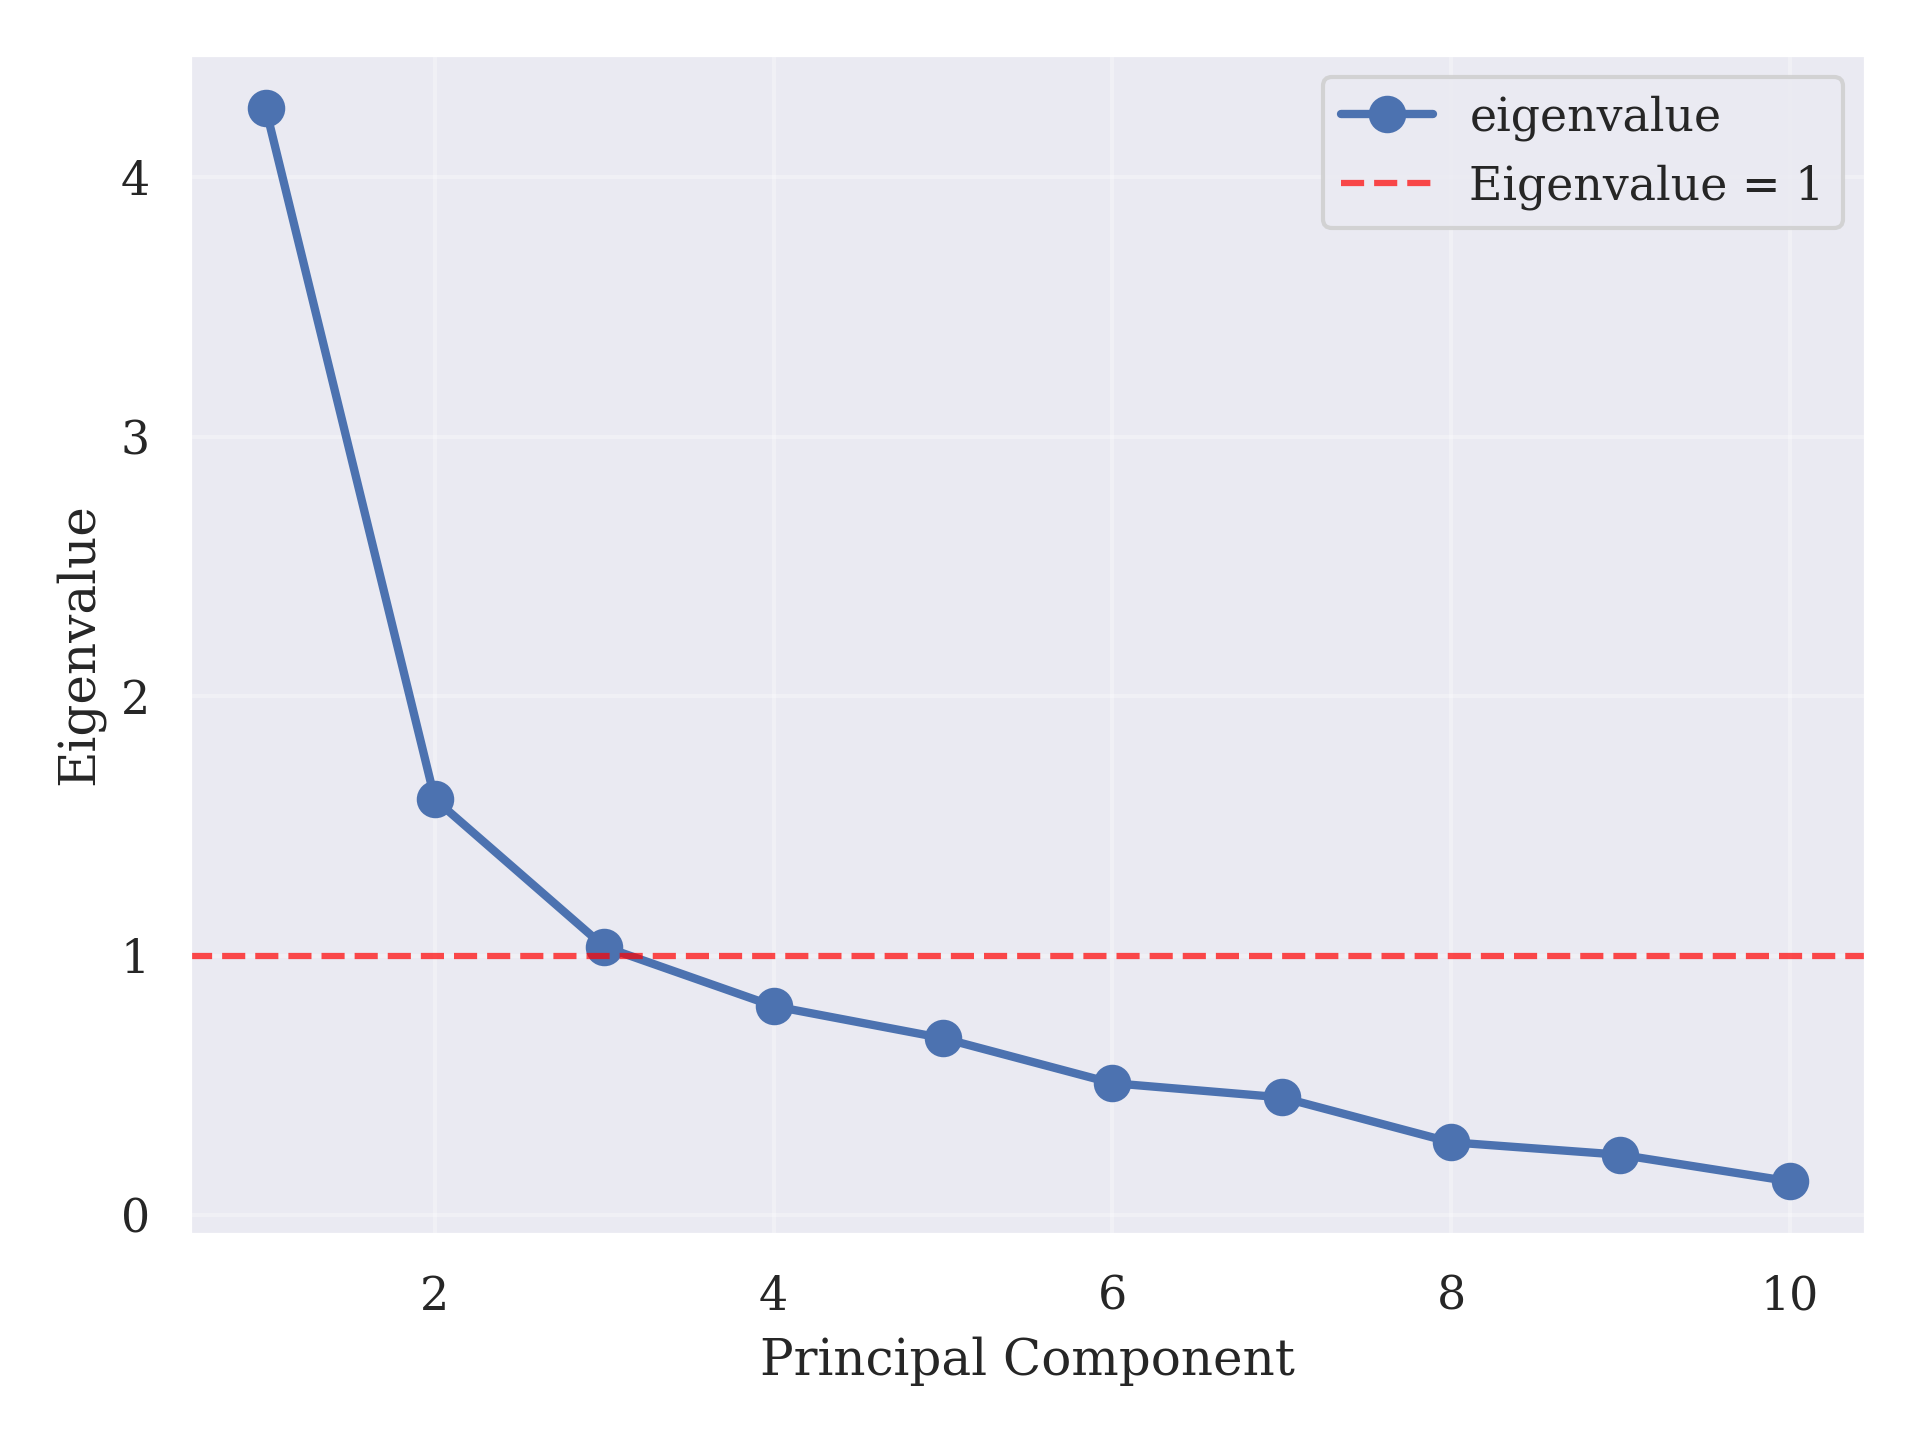
\includegraphics[width=0.9\linewidth]{thesis_images/04RE_scree_plot_eigenvalues} 

}

\caption{ PCA Scree Plot }\label{fig:04RE-pca-scree}
\end{figure}

\begin{figure}

{\centering 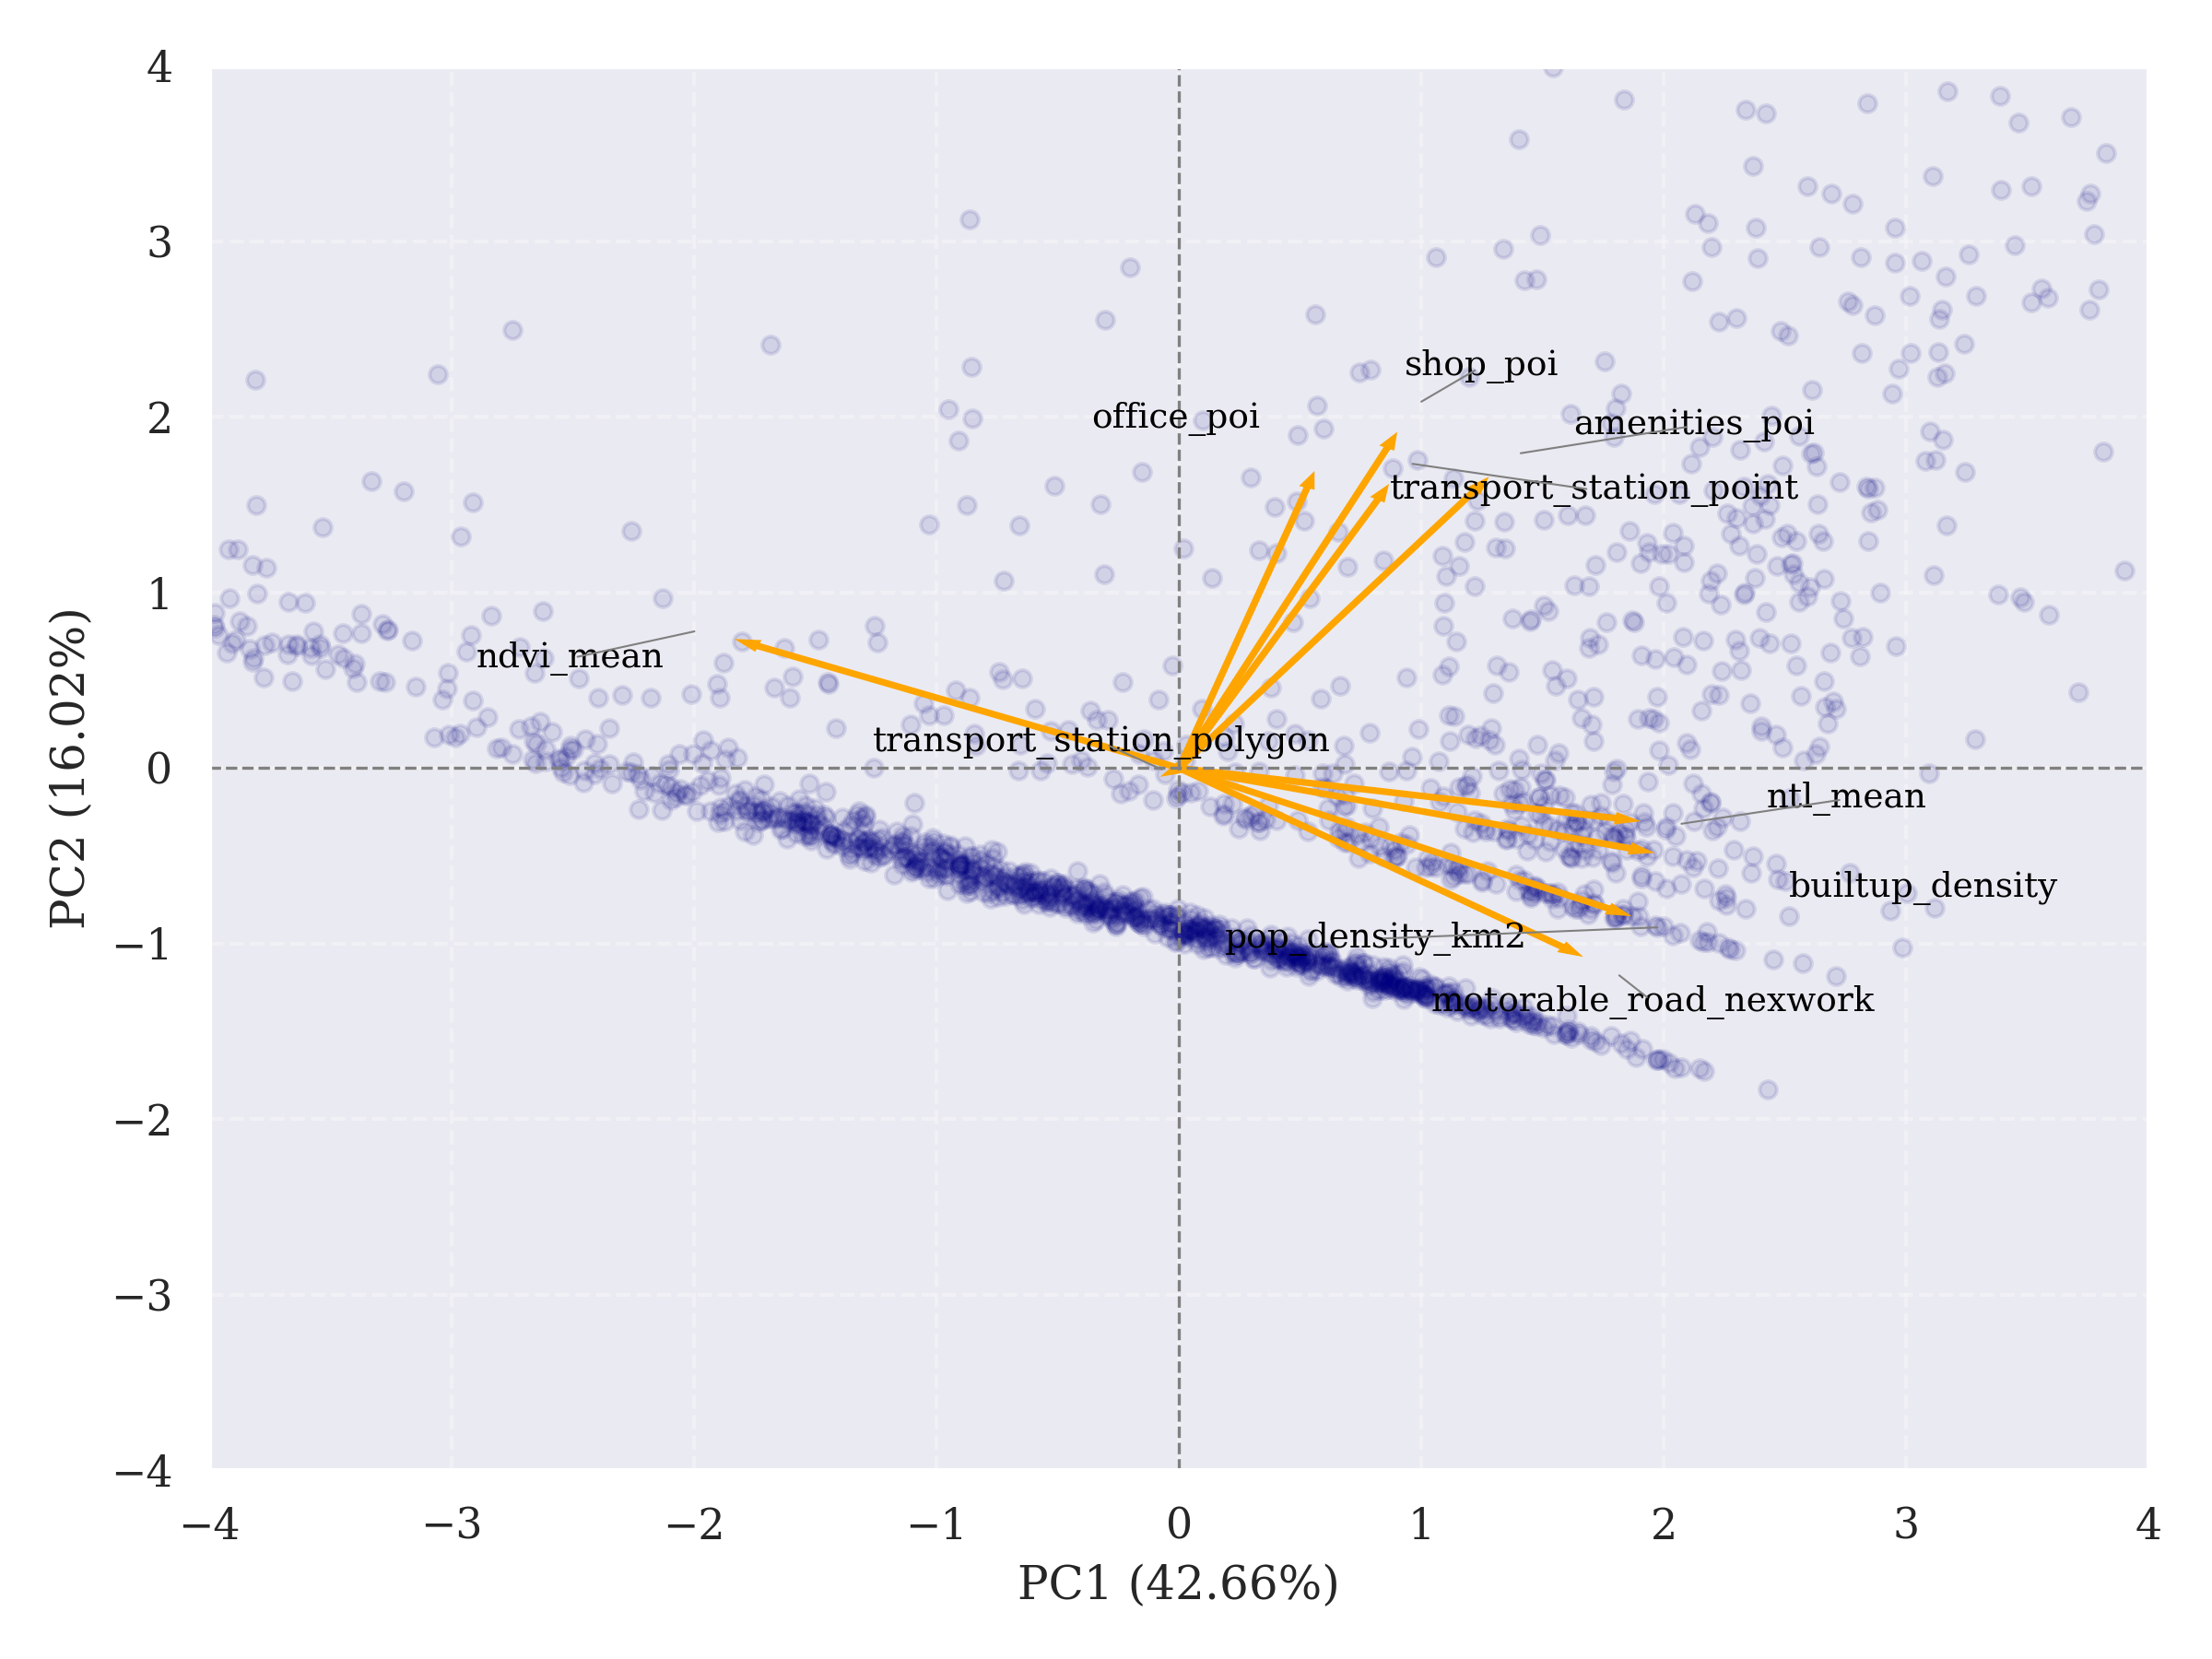
\includegraphics[width=0.9\linewidth]{thesis_images/04RE_pca_biplot} 

}

\caption{ PCA Biplot }\label{fig:04RE-pca-biplot}
\end{figure}

\setlength{\tabcolsep}{4pt}

\begingroup\fontsize{9}{11}\selectfont

\begin{longtable}[t]{p{0.40\linewidth}>{\raggedleft\arraybackslash}p{0.30\linewidth}>{\raggedleft\arraybackslash}p{0.30\linewidth}}
\caption{\label{tab:pca-loadings}Principal Component Loadings for Indicators}\\
\toprule
\textbf{Variable} & \textbf{PC1 Loading} & \textbf{PC2 Loading}\\
\midrule
\endfirsthead
\caption[]{\label{tab:pca-loadings}Principal Component Loadings for Indicators \textit{(continued)}}\\
\toprule
\textbf{Variable} & \textbf{PC1 Loading} & \textbf{PC2 Loading}\\
\midrule
\endhead

\endfoot
\bottomrule
\endlastfoot
builtup density & 0.432 & -0.126\\
ntl mean & 0.419 & -0.079\\
pop density km2 & 0.411 & -0.220\\
motorable road network & 0.367 & -0.280\\
amenities poi & 0.283 & 0.434\\
\addlinespace
shop poi & 0.199 & 0.502\\
transport station point & 0.191 & 0.423\\
office poi & 0.123 & 0.442\\
transport station polygon & -0.009 & -0.006\\
ndvi mean & -0.404 & 0.191\\*
\end{longtable}
\endgroup{}

\setlength{\tabcolsep}{6pt}

\subsection{Spatial Patterns of Economic Activity}\label{spatial-patterns-of-economic-activity}

Built on the first principal component (PC1), an Economic Activity Index (EAI) was mapped across 500 m hexagonal grids (Figure \ref{fig:04RE-eai}). The resulting surface shows a continuous gradient of economic intensity across Jaipur. Highest values concentrate in the historic core and along major built-up corridors, while intensity declines progressively toward the periphery. Very low values appear in the northeast around mountainous and green areas such as Nahargarh and along city edges, where boundary truncation may accentuate discontinuities. This gradient broadly mirrors the distribution of population density and built-up extent, reinforcing the interpretation of PC1 as a proxy for urban economic activity.

While the EAI emphasises a smooth core--periphery gradient, k-means clustering of PC1--PC2 scores (k = 3) reveals discrete structural groupings within the city (Figure \ref{fig:04RE-eai-cluster}, Figure \ref{fig:04RE-eai-cluster-cate} and Figure \ref{fig:04RE-eai-cluster-spa}):

\begin{itemize}
\tightlist
\item
  \textbf{Cluster 1 :} localised high-activity zones, often aligned with secondary centres and transport-accessible sub-districts.
\item
  \textbf{Cluster 2 :} the bulk of the built-up fabric, representing medium-intensity areas with balanced but not extreme economic activity.
\item
  \textbf{Cluster 3 :} peripheral low-activity zones, concentrated in hilly or green terrain and forming a distinct ecological type.
\end{itemize}

These two perspectives are complementary: the EAI captures the overall intensity gradient, while clustering differentiates categorical spatial types. This dual representation provides both a citywide overview of economic activity and the identification of distinct functional zones within Jaipur.

\begin{figure}

{\centering 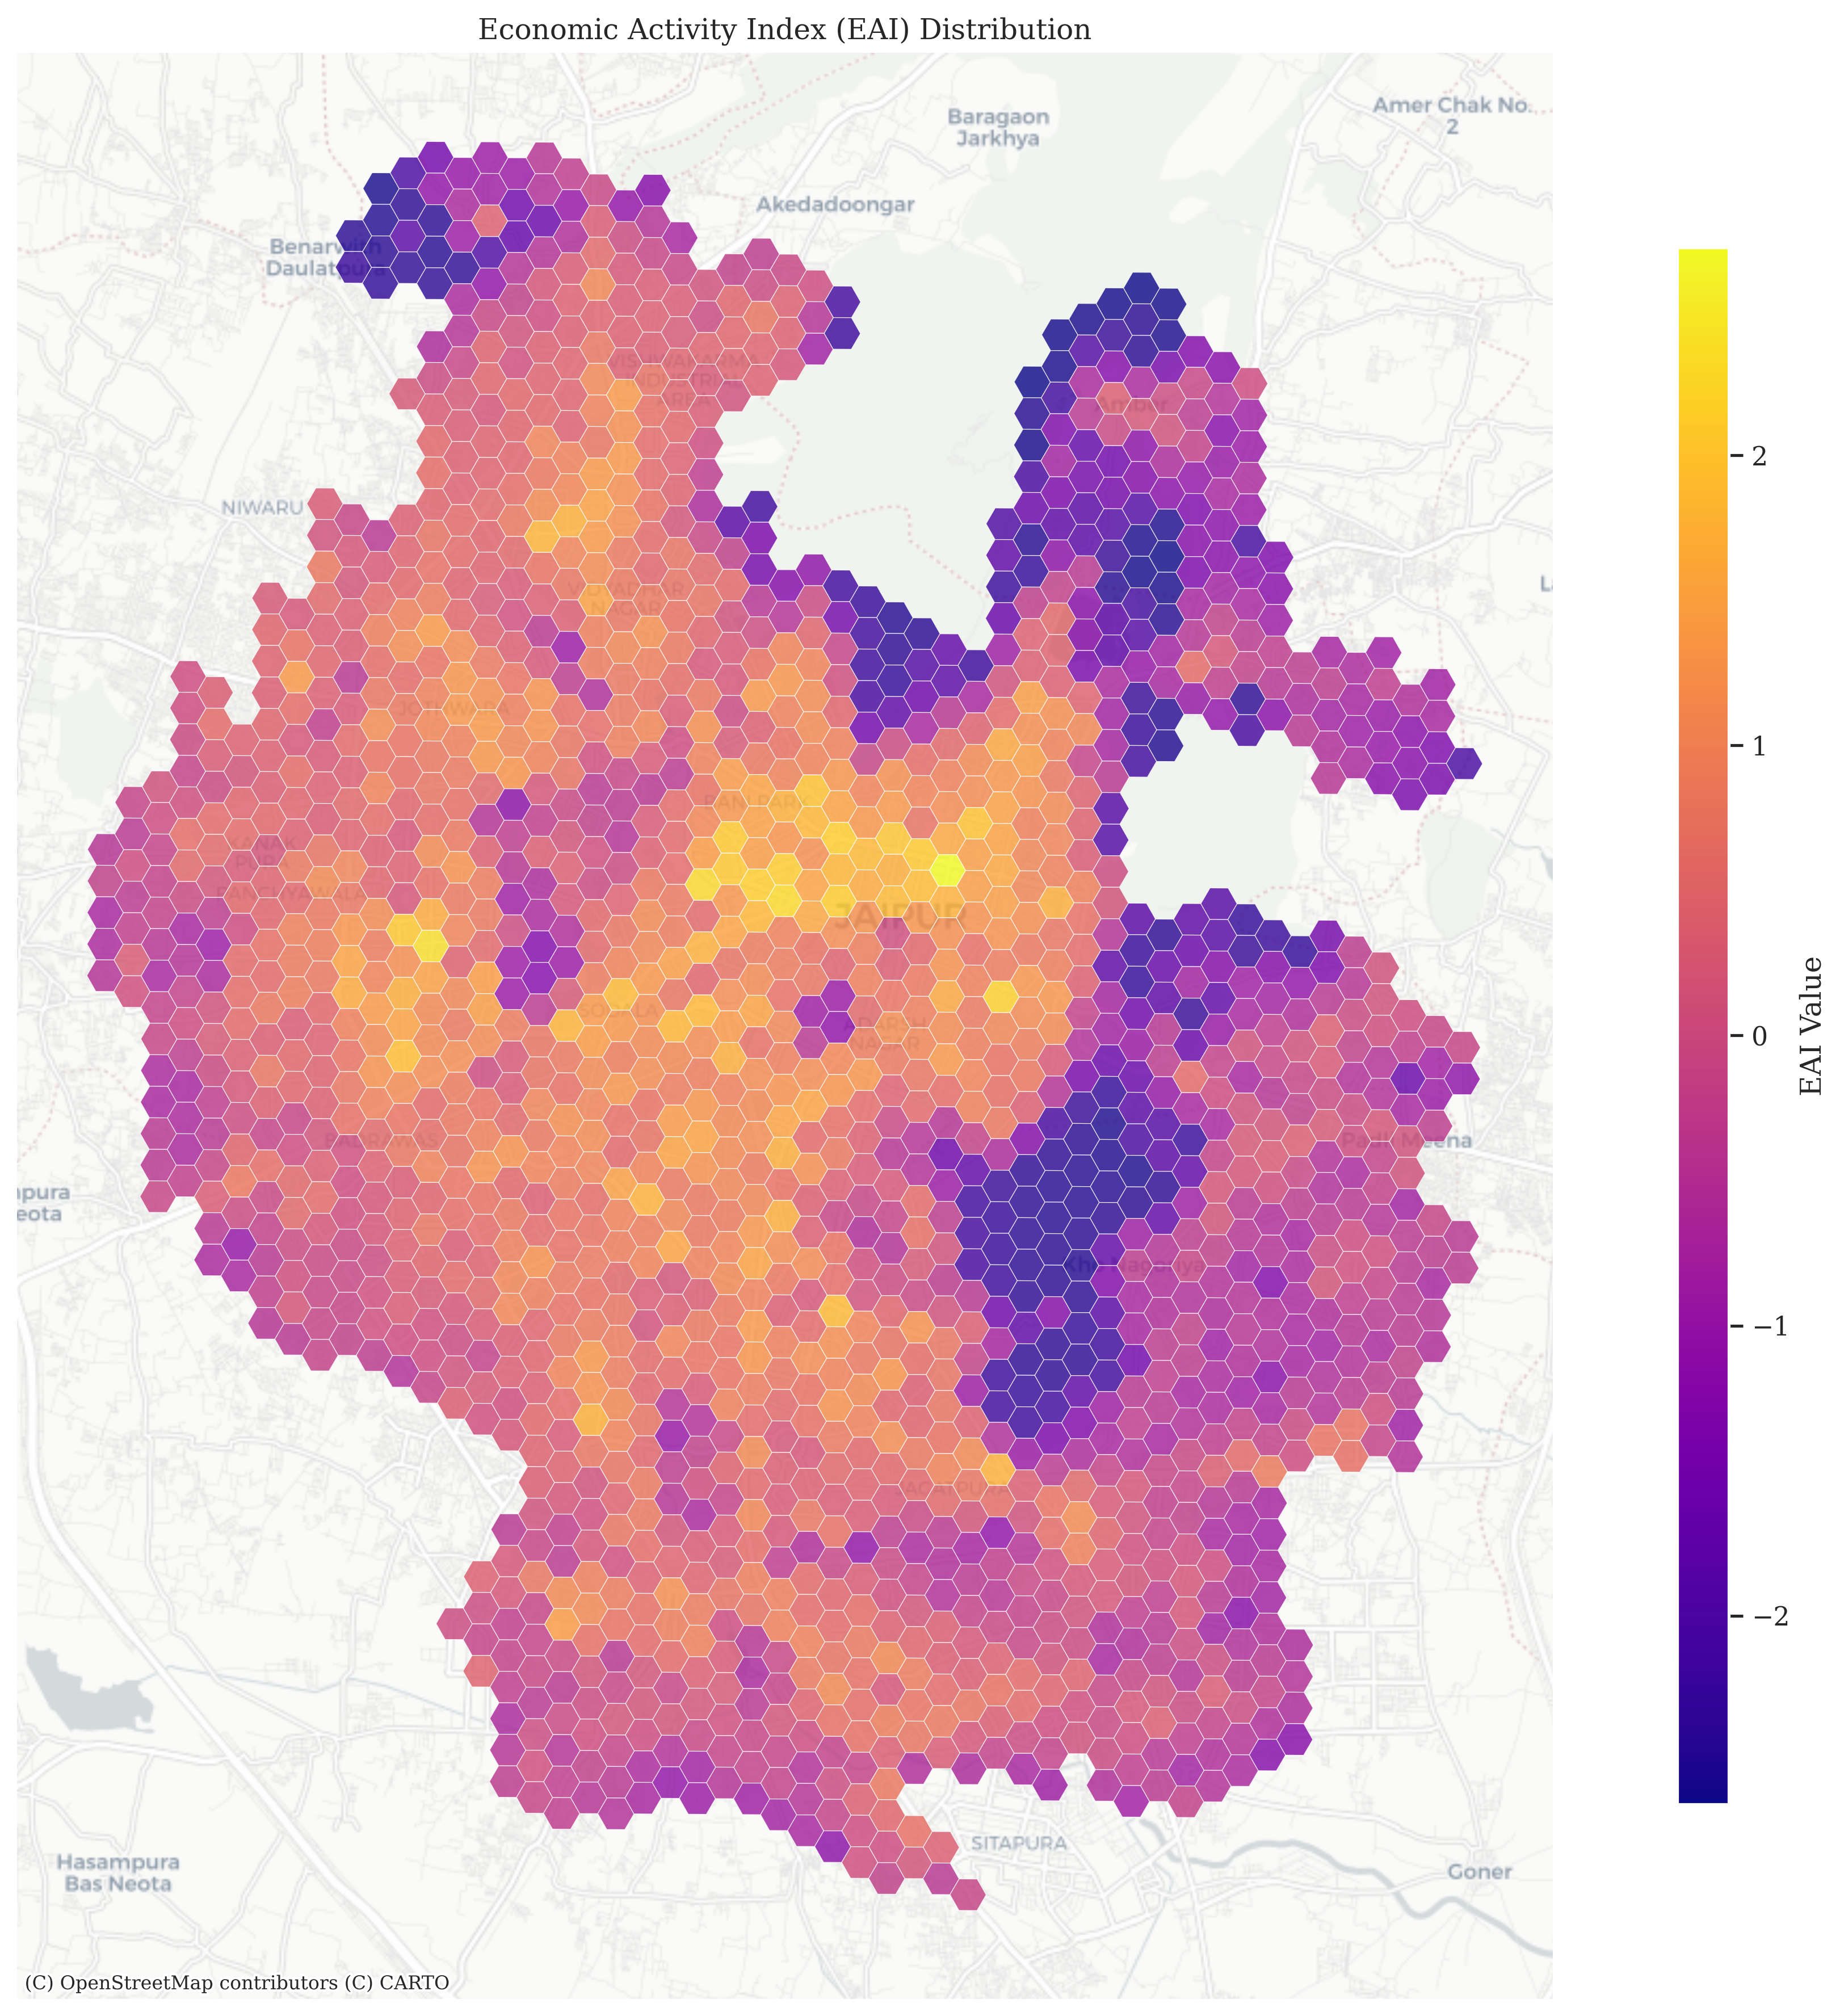
\includegraphics[width=0.98\linewidth]{thesis_images/04RE_eai_distribution_map} 

}

\caption{ Economic Activity Index (EAI) Distribution }\label{fig:04RE-eai}
\end{figure}

\begin{figure}

{\centering 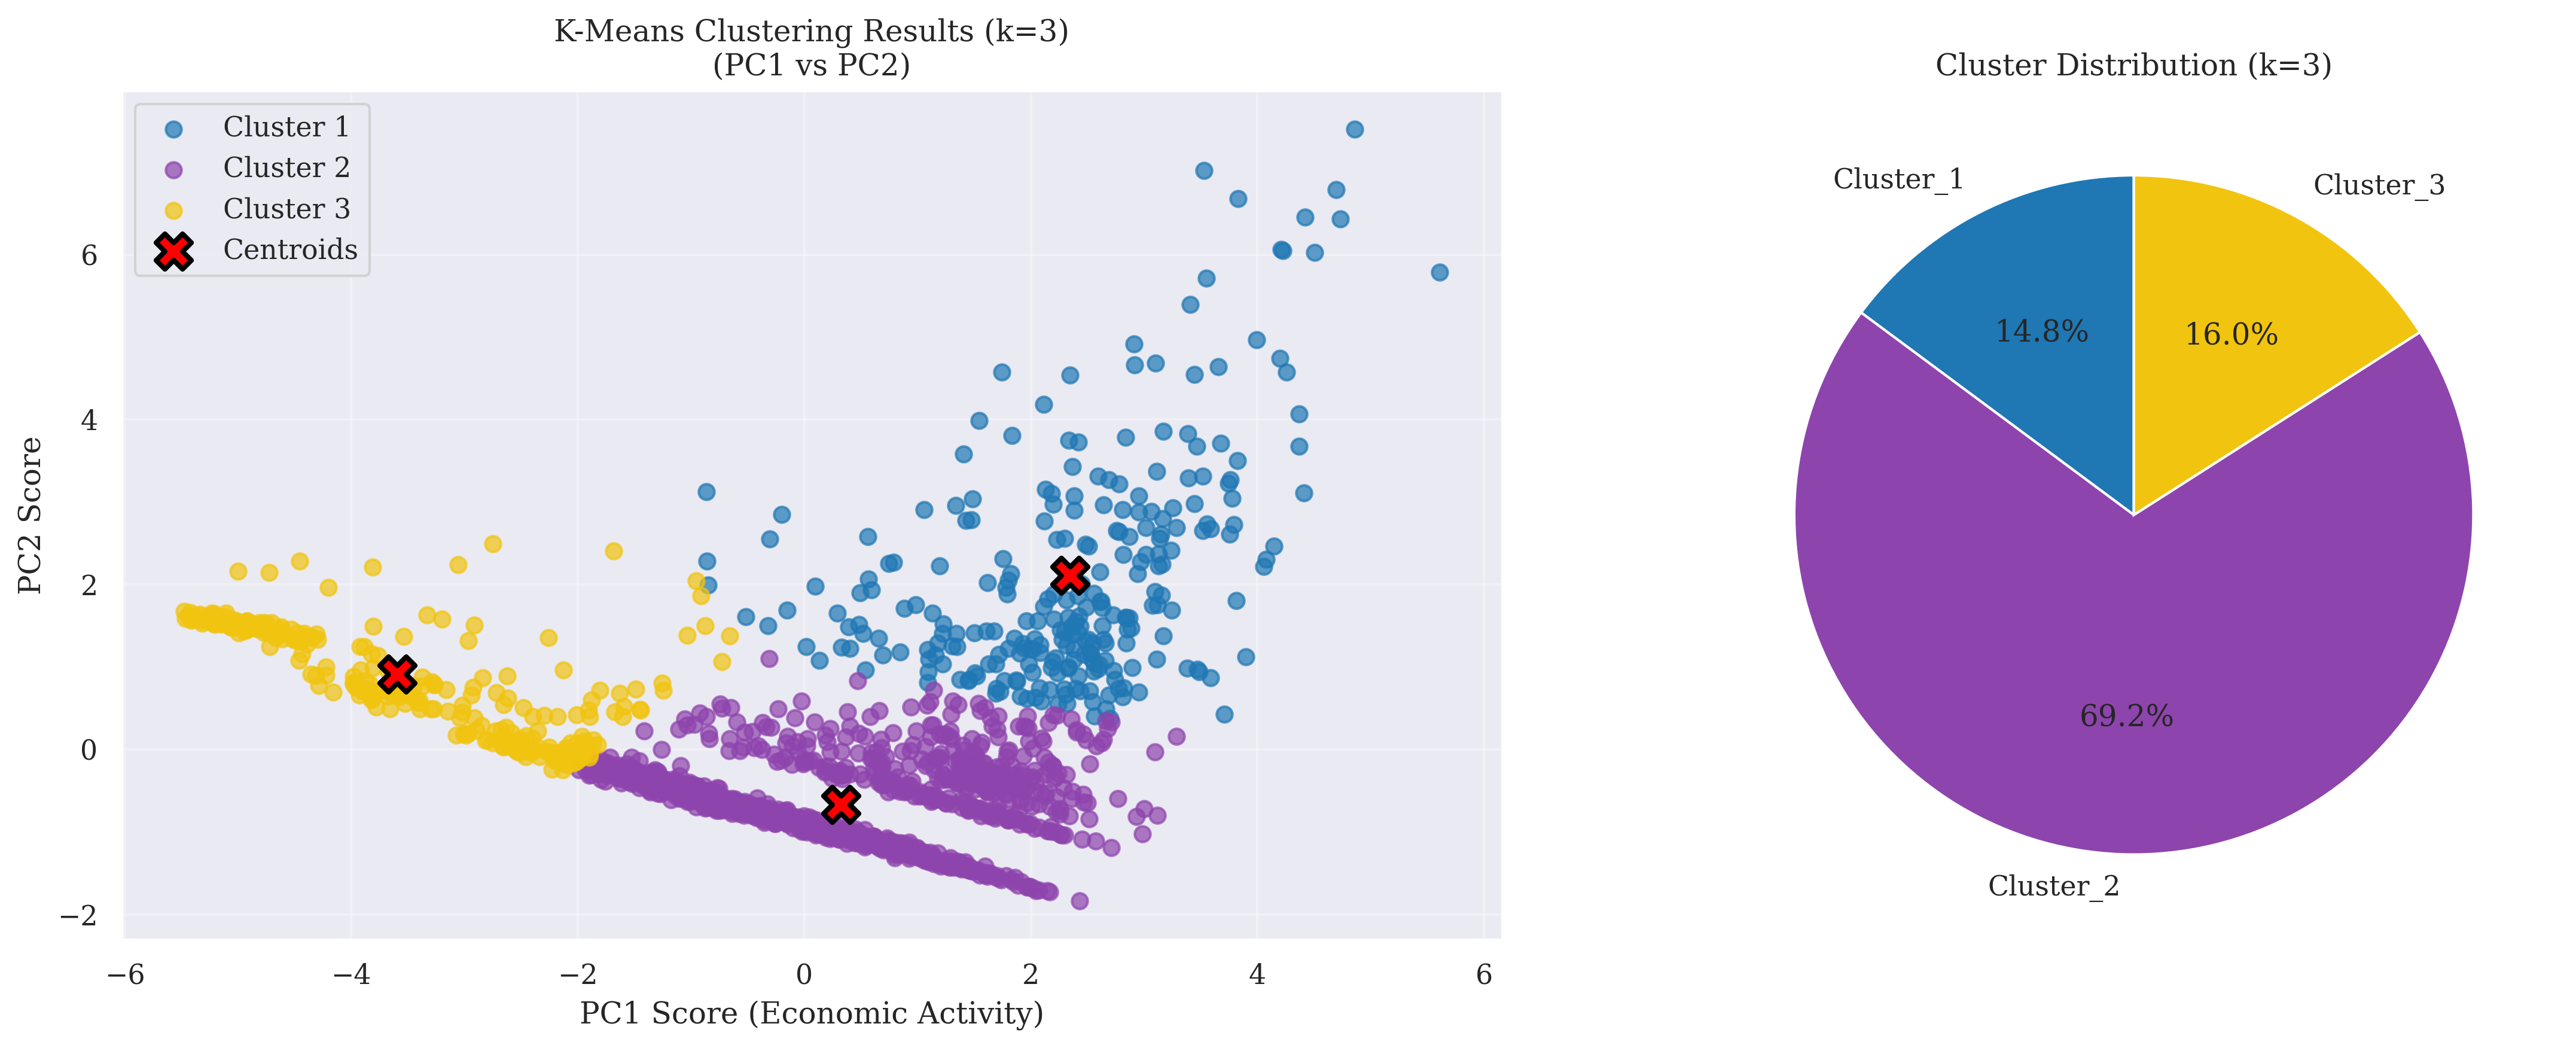
\includegraphics[width=0.98\linewidth]{thesis_images/04RE_kmeans_clustering_results} 

}

\caption{ K-Means Clustering Results for EAI }\label{fig:04RE-eai-cluster}
\end{figure}

\begin{figure}

{\centering 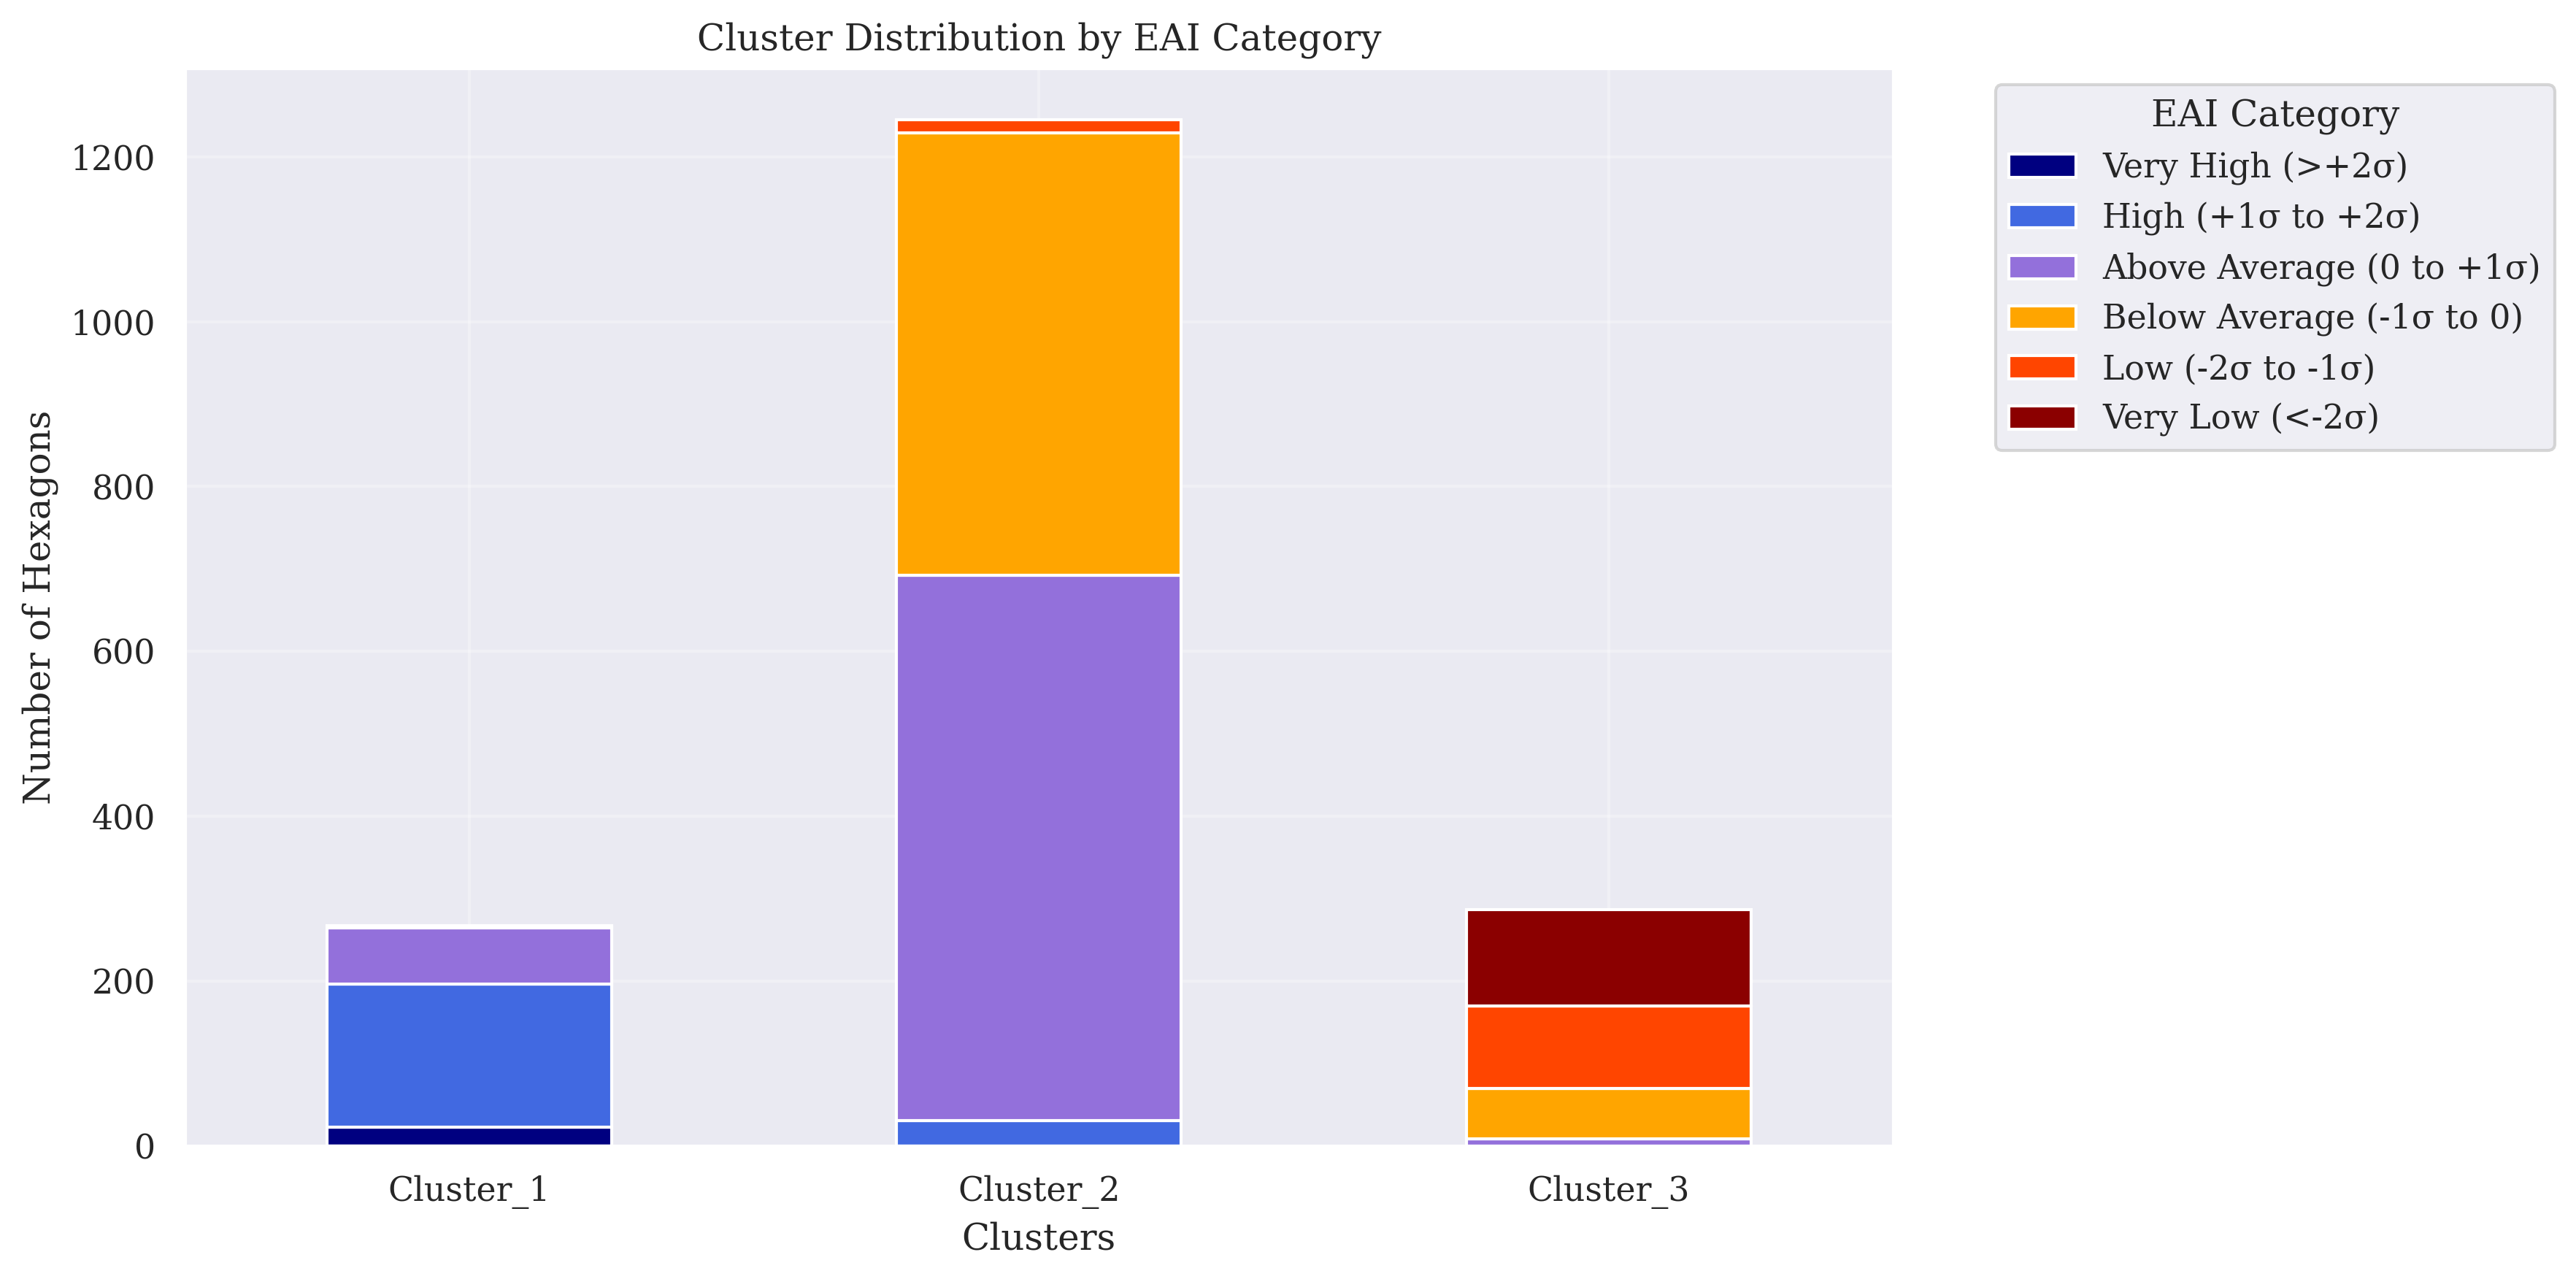
\includegraphics[width=0.98\linewidth]{thesis_images/04RE_cluster_vs_epi_distribution} 

}

\caption{ Composition of K-Means Clusters for EAI. Legend categories reflect z-score-based classification of EAI values.}\label{fig:04RE-eai-cluster-cate}
\end{figure}

\begin{figure}

{\centering 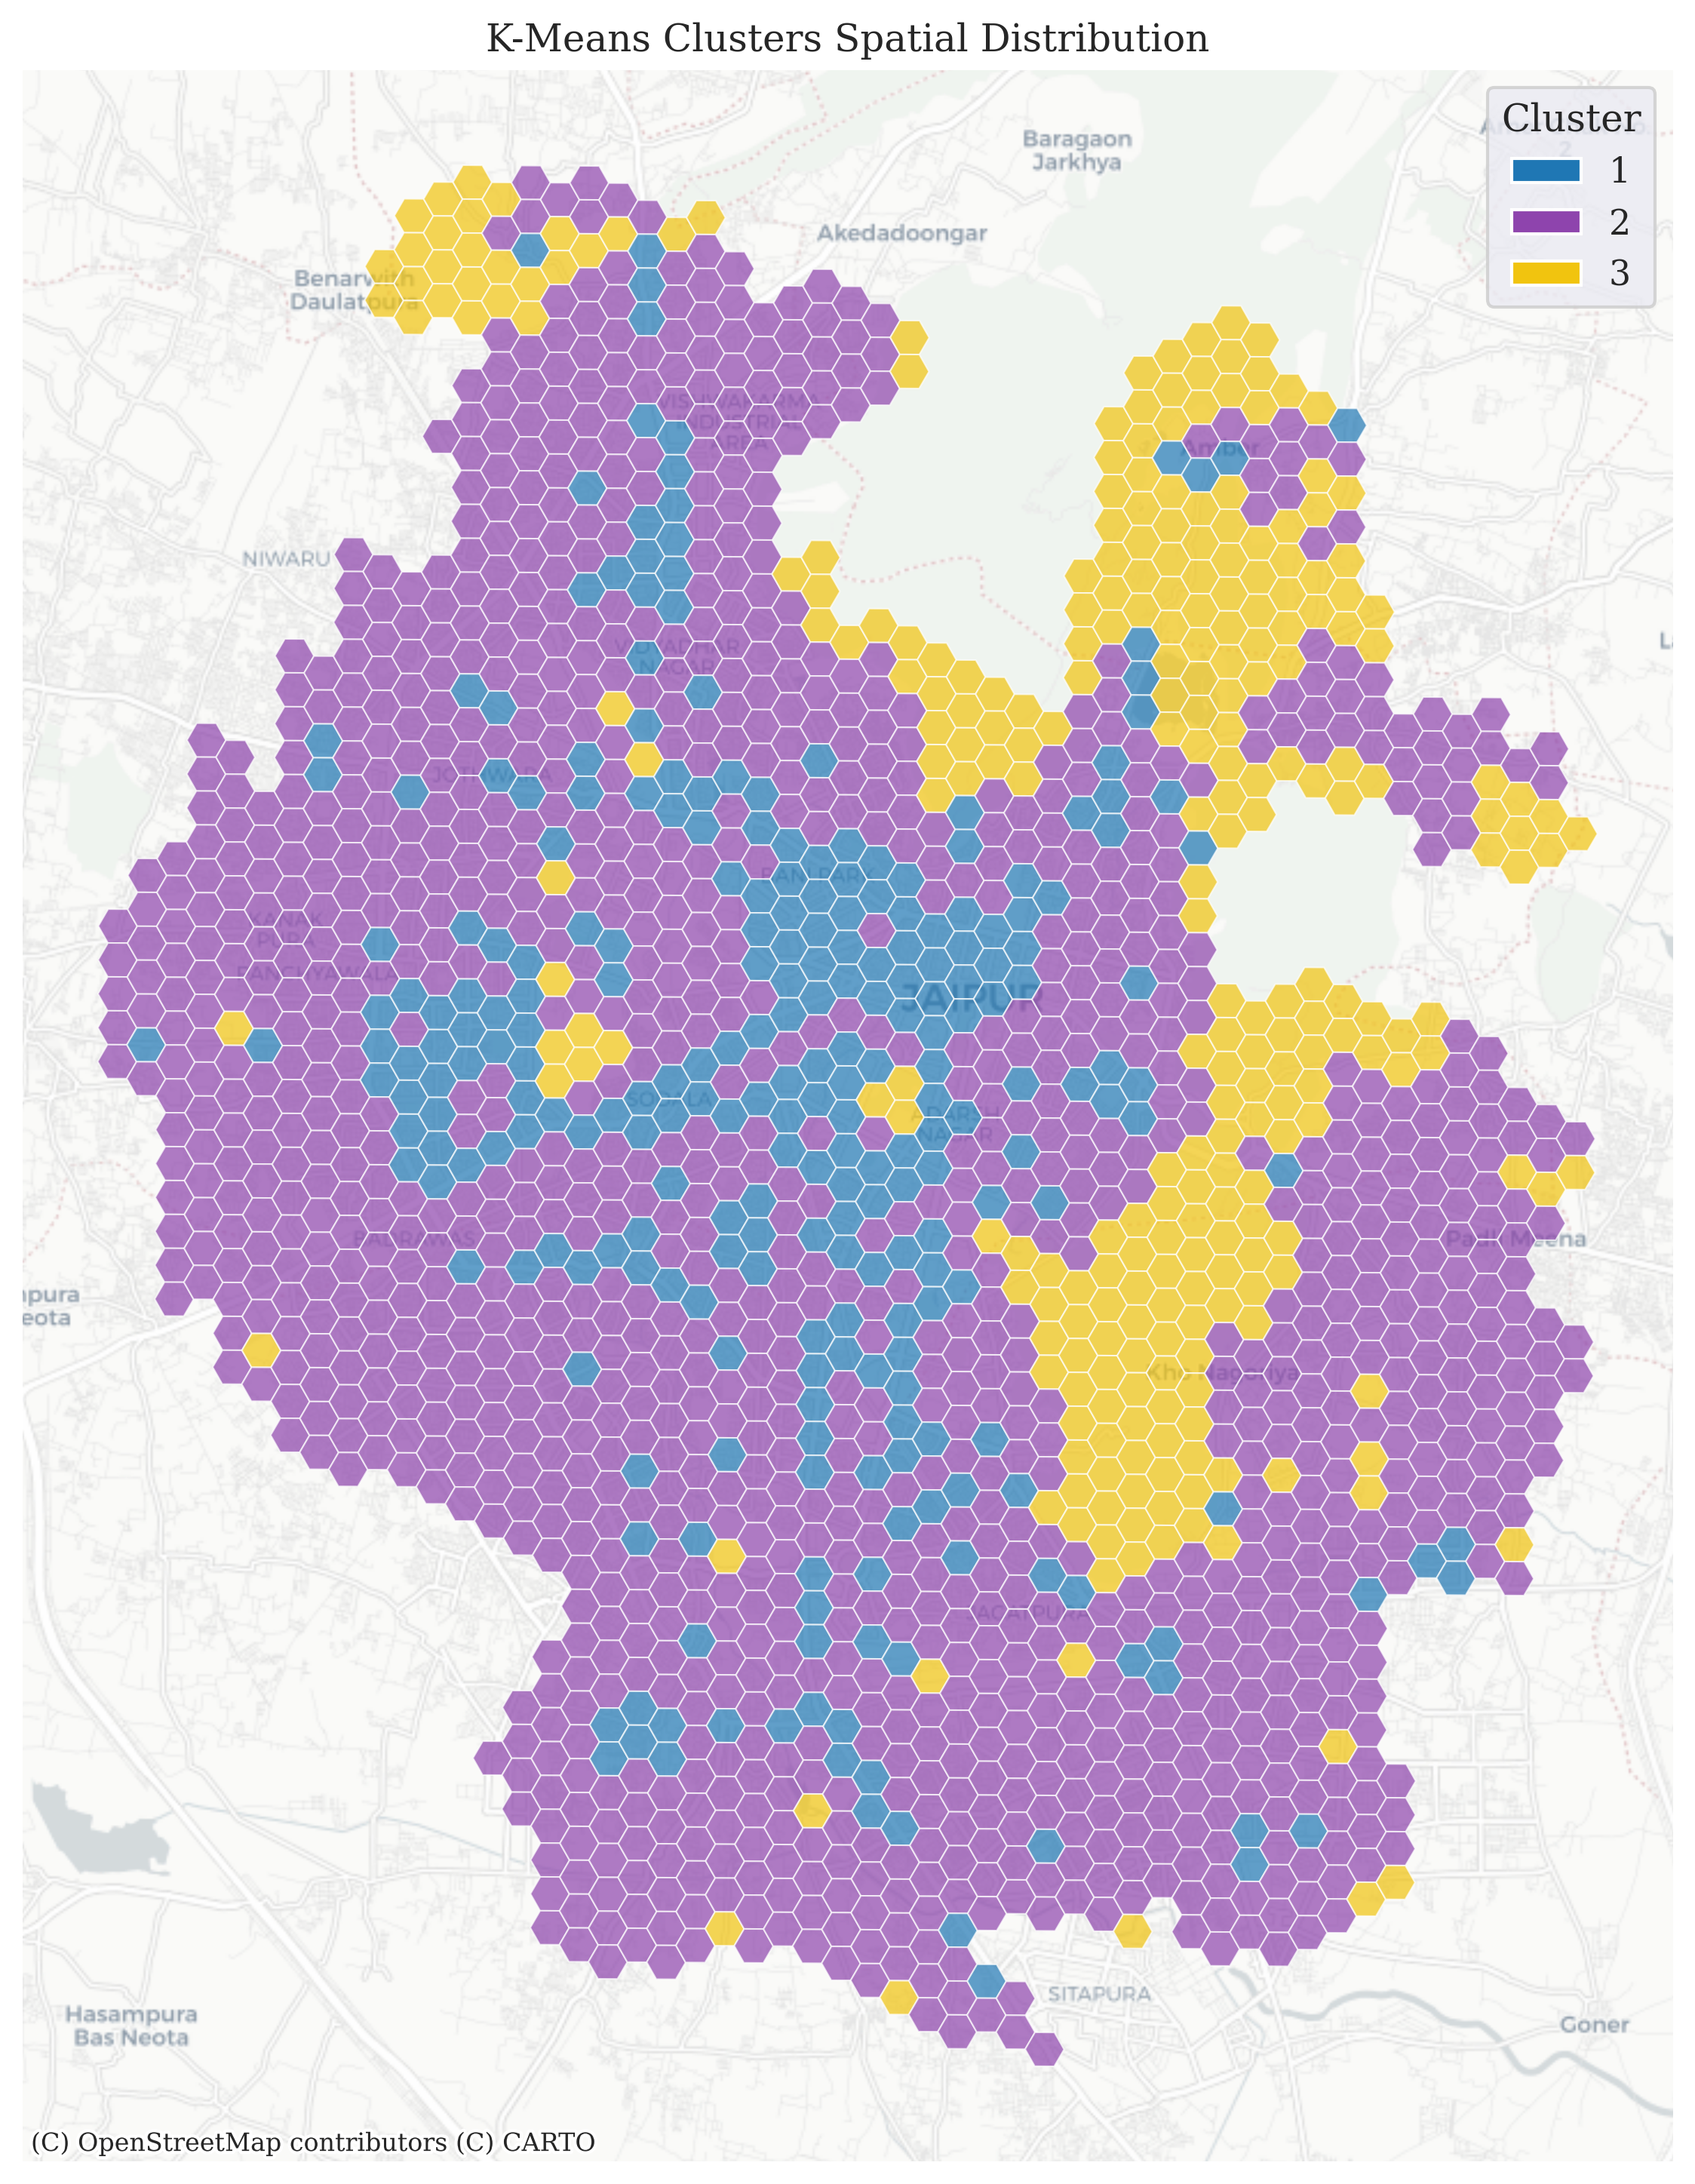
\includegraphics[width=0.98\linewidth]{thesis_images/04RE_kmeans_clusters_map} 

}

\caption{ K-Means Clusters Spatial Distribution for EAI }\label{fig:04RE-eai-cluster-spa}
\end{figure}

\section{Response to RQ2: GEE -- Jaipur Urban Activities Analysis App}\label{response-to-rq2-gee-jaipur-urban-activities-analysis-app}

To address the second research question, the outputs of the MGWR-based population disaggregation and the Economic Activity Index (EAI) were embedded into an interactive Google Earth Engine (GEE) web application (Figure \ref{fig:04RE-geeapp}). Without delving into technical implementation, the app is presented as a proof of concept, showing how analytical outputs can be translated into a transparent and accessible tool for digital planning. . By allowing stakeholders to explore and interpret spatial data directly in a browser, the app lowers the technical barriers posed by conventional GIS software and supports more inclusive, evidence-based dialogue.

The application demonstrates three ways in which results can be mobilised for planning:

\begin{itemize}
\tightlist
\item
  \textbf{Comparing neighbourhood populations:} Users can draw custom polygons and instantly obtain population counts and histograms. This flexibility allows comparisons beyond ward boundaries, supporting discussions of uneven population densities and local service demand.
\item
  \textbf{Highlighting economic contrasts:} Ward-level aggregation ranks areas by their average EAI, displaying the top ten as a clear entry point for identifying economic hotspots and areas of relative deprivation. This ranking function transforms abstract indices into a straightforward narrative of concentration and disparity.
\item
  \textbf{Interrogating indicator contributions:} Users can switch between NDVI, nighttime lights, and road density layers to see how each indicator contributes to the composite EAI. This transparency enables scrutiny of the underlying assumptions and encourages informed debate on the drivers of urban economic activity.
\end{itemize}

These functions transform static analytical results into an interactive platform that is meaningful for both experts and non-experts. For planners, the app provides rapid access to disaggregated data without specialised software; for communities, it renders complex indicators into intuitive visualisations. In this way, the Jaipur Urban Activities Analysis App demonstrates how geospatial analysis, when coupled with cloud-based dissemination, can bridge the gap between technical research and public participation.

\FloatBarrier

\begin{figure}[H]

{\centering \subfloat[Application home page\label{fig:04RE-geeapp-1}]{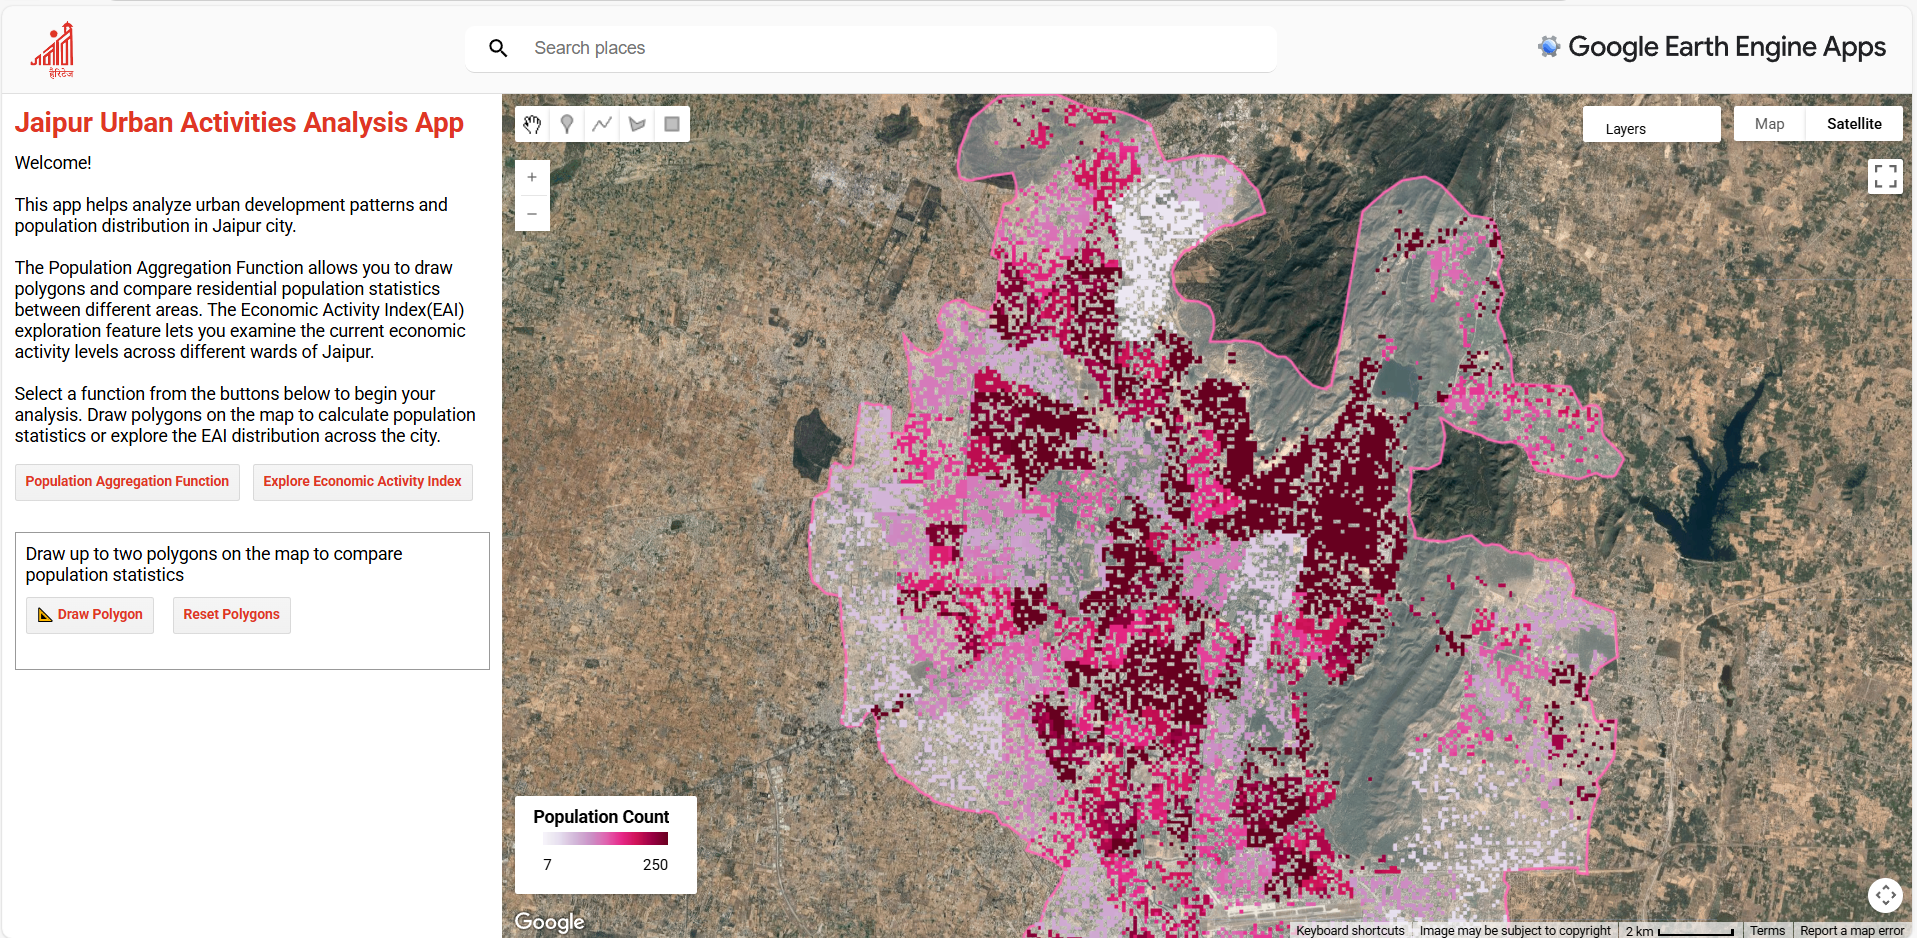
\includegraphics[width=0.48\linewidth]{thesis_images/04RE_geeapp_01} }\subfloat[Polygon-based population comparison\label{fig:04RE-geeapp-2}]{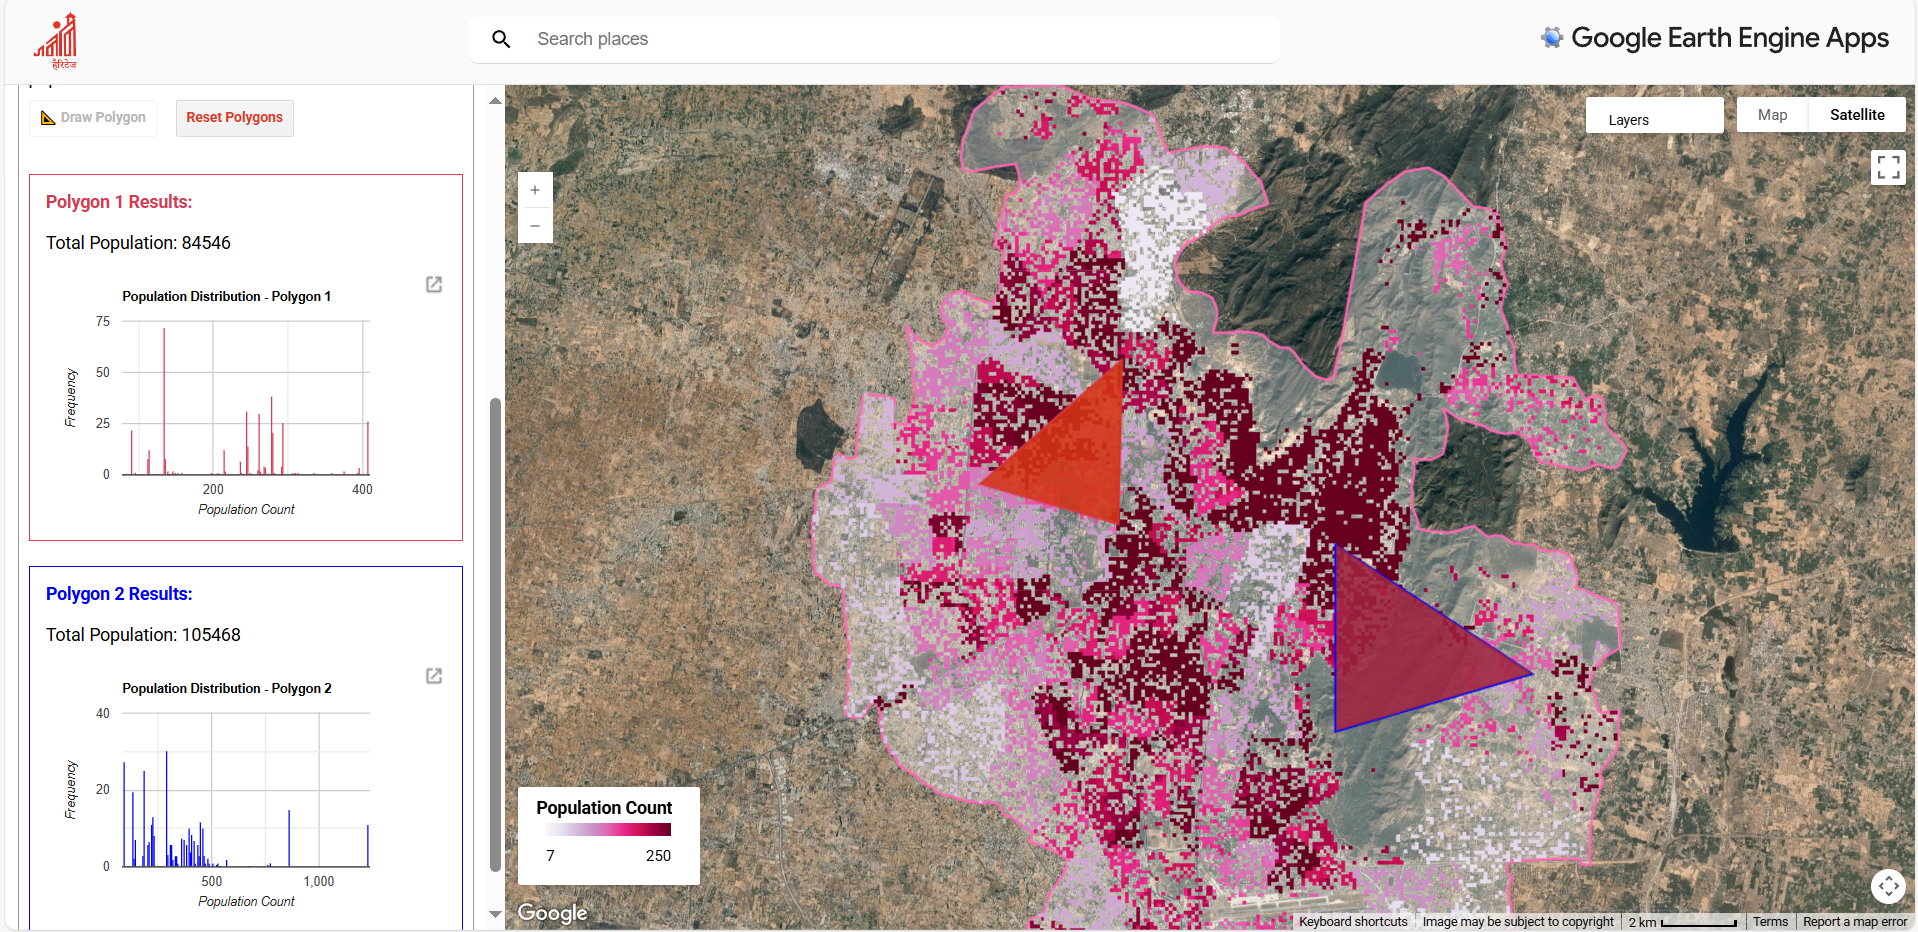
\includegraphics[width=0.48\linewidth]{thesis_images/04RE_geeapp_02} }\newline\subfloat[Ward-based EAI aggregation\label{fig:04RE-geeapp-3}]{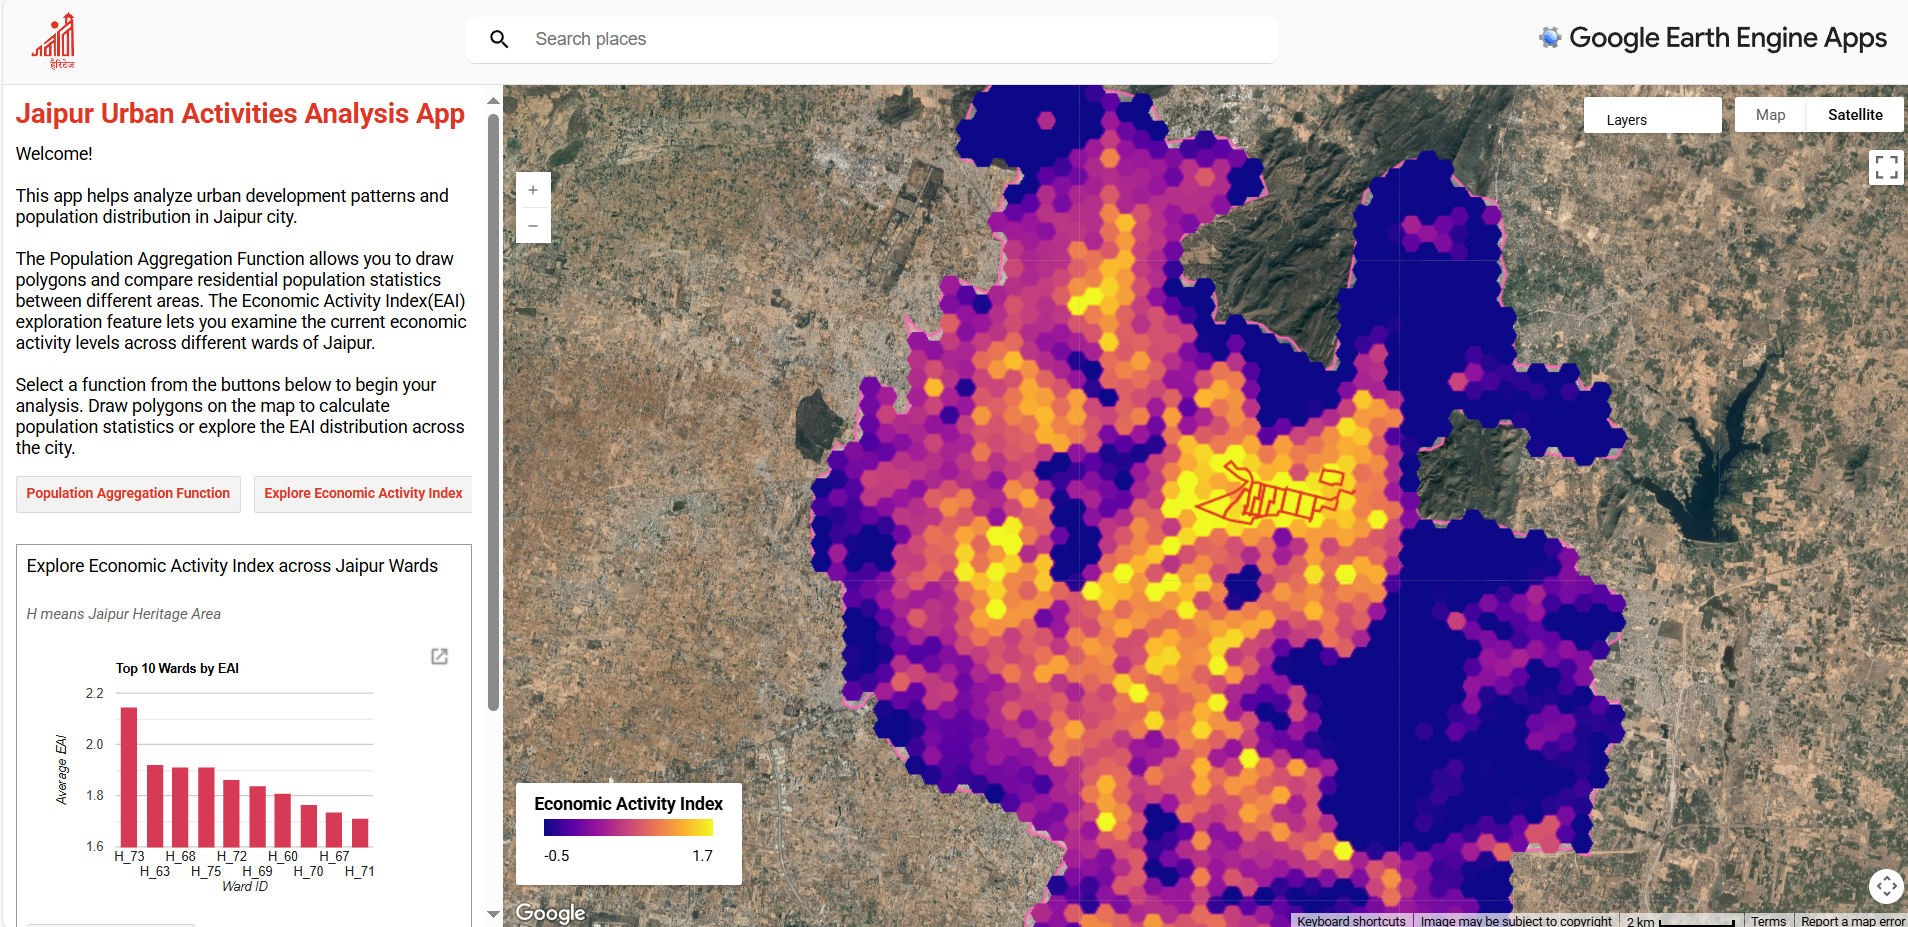
\includegraphics[width=0.48\linewidth]{thesis_images/04RE_geeapp_03} }\subfloat[Variable distribution mapping (nighttime lights)\label{fig:04RE-geeapp-4}]{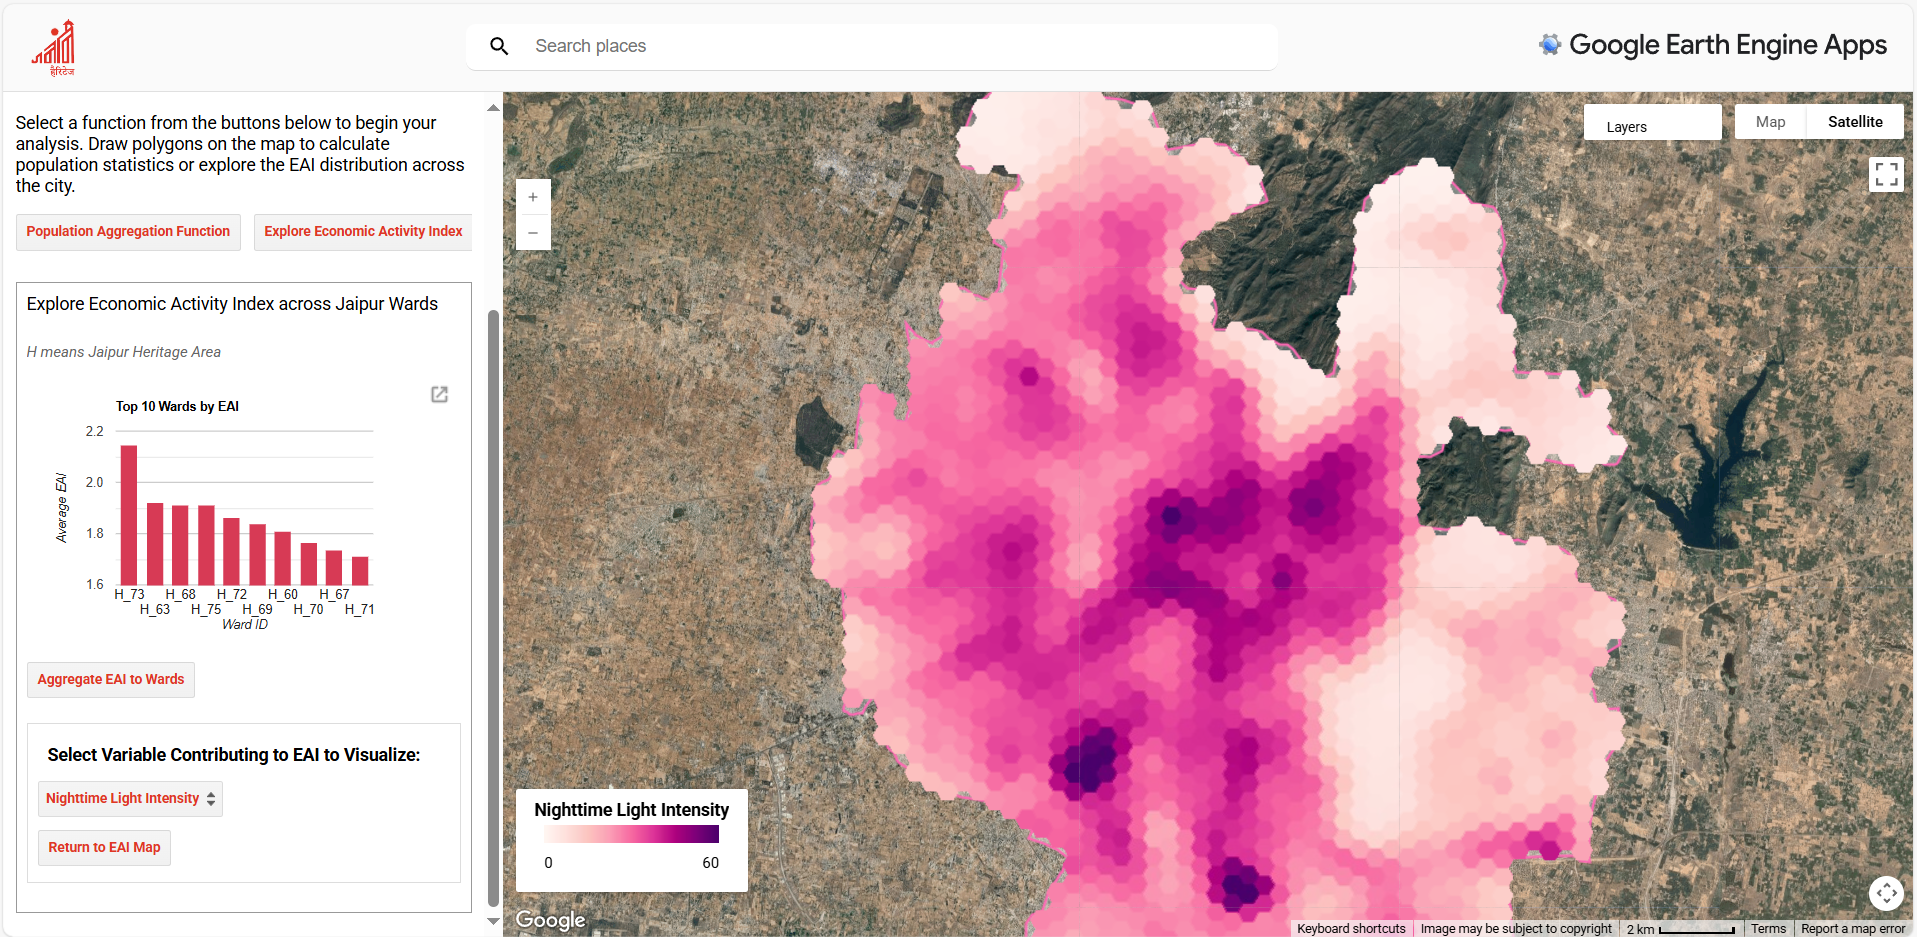
\includegraphics[width=0.48\linewidth]{thesis_images/04RE_geeapp_04} }\newline

}

\caption{Screenshots of the Interactive Google Earth Engine (GEE) Web Application Developed for This Study. Access link in GitHub repo.}\label{fig:04RE-geeapp}
\end{figure}

The findings across RQ1 and RQ2 demonstrate that remote sensing and open data can be effectively harnessed to estimate urban population distribution and economic activity in Jaipur, and that these outputs can be implemented into an accessible web application. Together, the analyses establish both methodological feasibility in a data-scarce context and practical relevance through interactive dissemination. Building on these results, the following Discussion reflects on their implications, limitations, and broader significance for digital urban planning.

\chapter{Discussion}\label{discussion}

\section{Evaluating Population Disaggregation: Strengths and Localised Biases}\label{evaluating-population-disaggregation-strengths-and-localised-biases}

The MGWR-based disaggregation of residential population reproduced Jaipur's overall settlement structure and corresponded well with GHSL benchmarks across much of the distribution. Residual analysis, however, revealed systematic deviations: dense zones were often overestimated, while environmentally constrained or low-density areas were underestimated. These biases reflect both the inherent limits of remote sensing proxies---nighttime lights, building volume, and POI kernel density---and the restricted variable sets, which cannot capture the full drivers of population variation.

Overestimation was not confined to the city core. Central wards near the Walled City were inflated mainly by the combination of dense commercial POI and saturated nighttime lights, even though most buildings are only one or two storeys. Outside the core, similar inflation appeared in other contexts. Clusters of JDA Quarters---standardised three-storey housing estates built by the Jaipur Development Authority---were systematically assigned higher population than neighbouring peri-urban blocks of detached houses. Likewise, large transport hubs drew disproportionate allocations because of strong POI signals, despite having little residential stock nearby.

By contrast, underestimation occurred in three main settings. In the northern Aravalli fringes, hillside villages remained weak in all three proxies (low lights, low residential volume, sparse POI). Within the city, large and greener institutional or open complexes showed little residential signal, reducing estimates even where dwellings were present. In peri-urban agricultural zones, dispersed housing embedded in cropland also produced faint signals, despite census and imagery evidence of sustained habitation.

Two structural factors further reinforced these patterns. First, the residential mask excluded some areas in advance as non-residential. Where dwellings existed outside the mask, the population had to be concentrated into the remaining residential cells, inflating estimates there. Second, the proxies themselves reflect built and service intensity rather than actual occupancy. This left the model insensitive to underused housing stock and to residential uses embedded within non-residential settings.

Industrial and mixed-use environments showed especially mixed results. Some estates were overestimated, where industrial sheds, intense lighting, and business-related POI were misread as residential signals---such as several RIICO industrial blocks. Others were underestimated, where worker housing or embedded residences produced only weak proxy values---such as the Vishwakarma industrial area in the north. These contrasts highlight the ambiguity of proxies, where economic signals do not equate to residential population, and underline the absence of variables that could separate economic from residential land uses.

To illustrate how these mechanisms manifest across Jaipur, eight selected sites---four overestimated and four underestimated---are presented with satellite imagery and street-level views (Figure \ref{fig:05DI-8estimates-01} and Figure \ref{fig:05DI-8estimates-02}).

\begin{figure}

{\centering 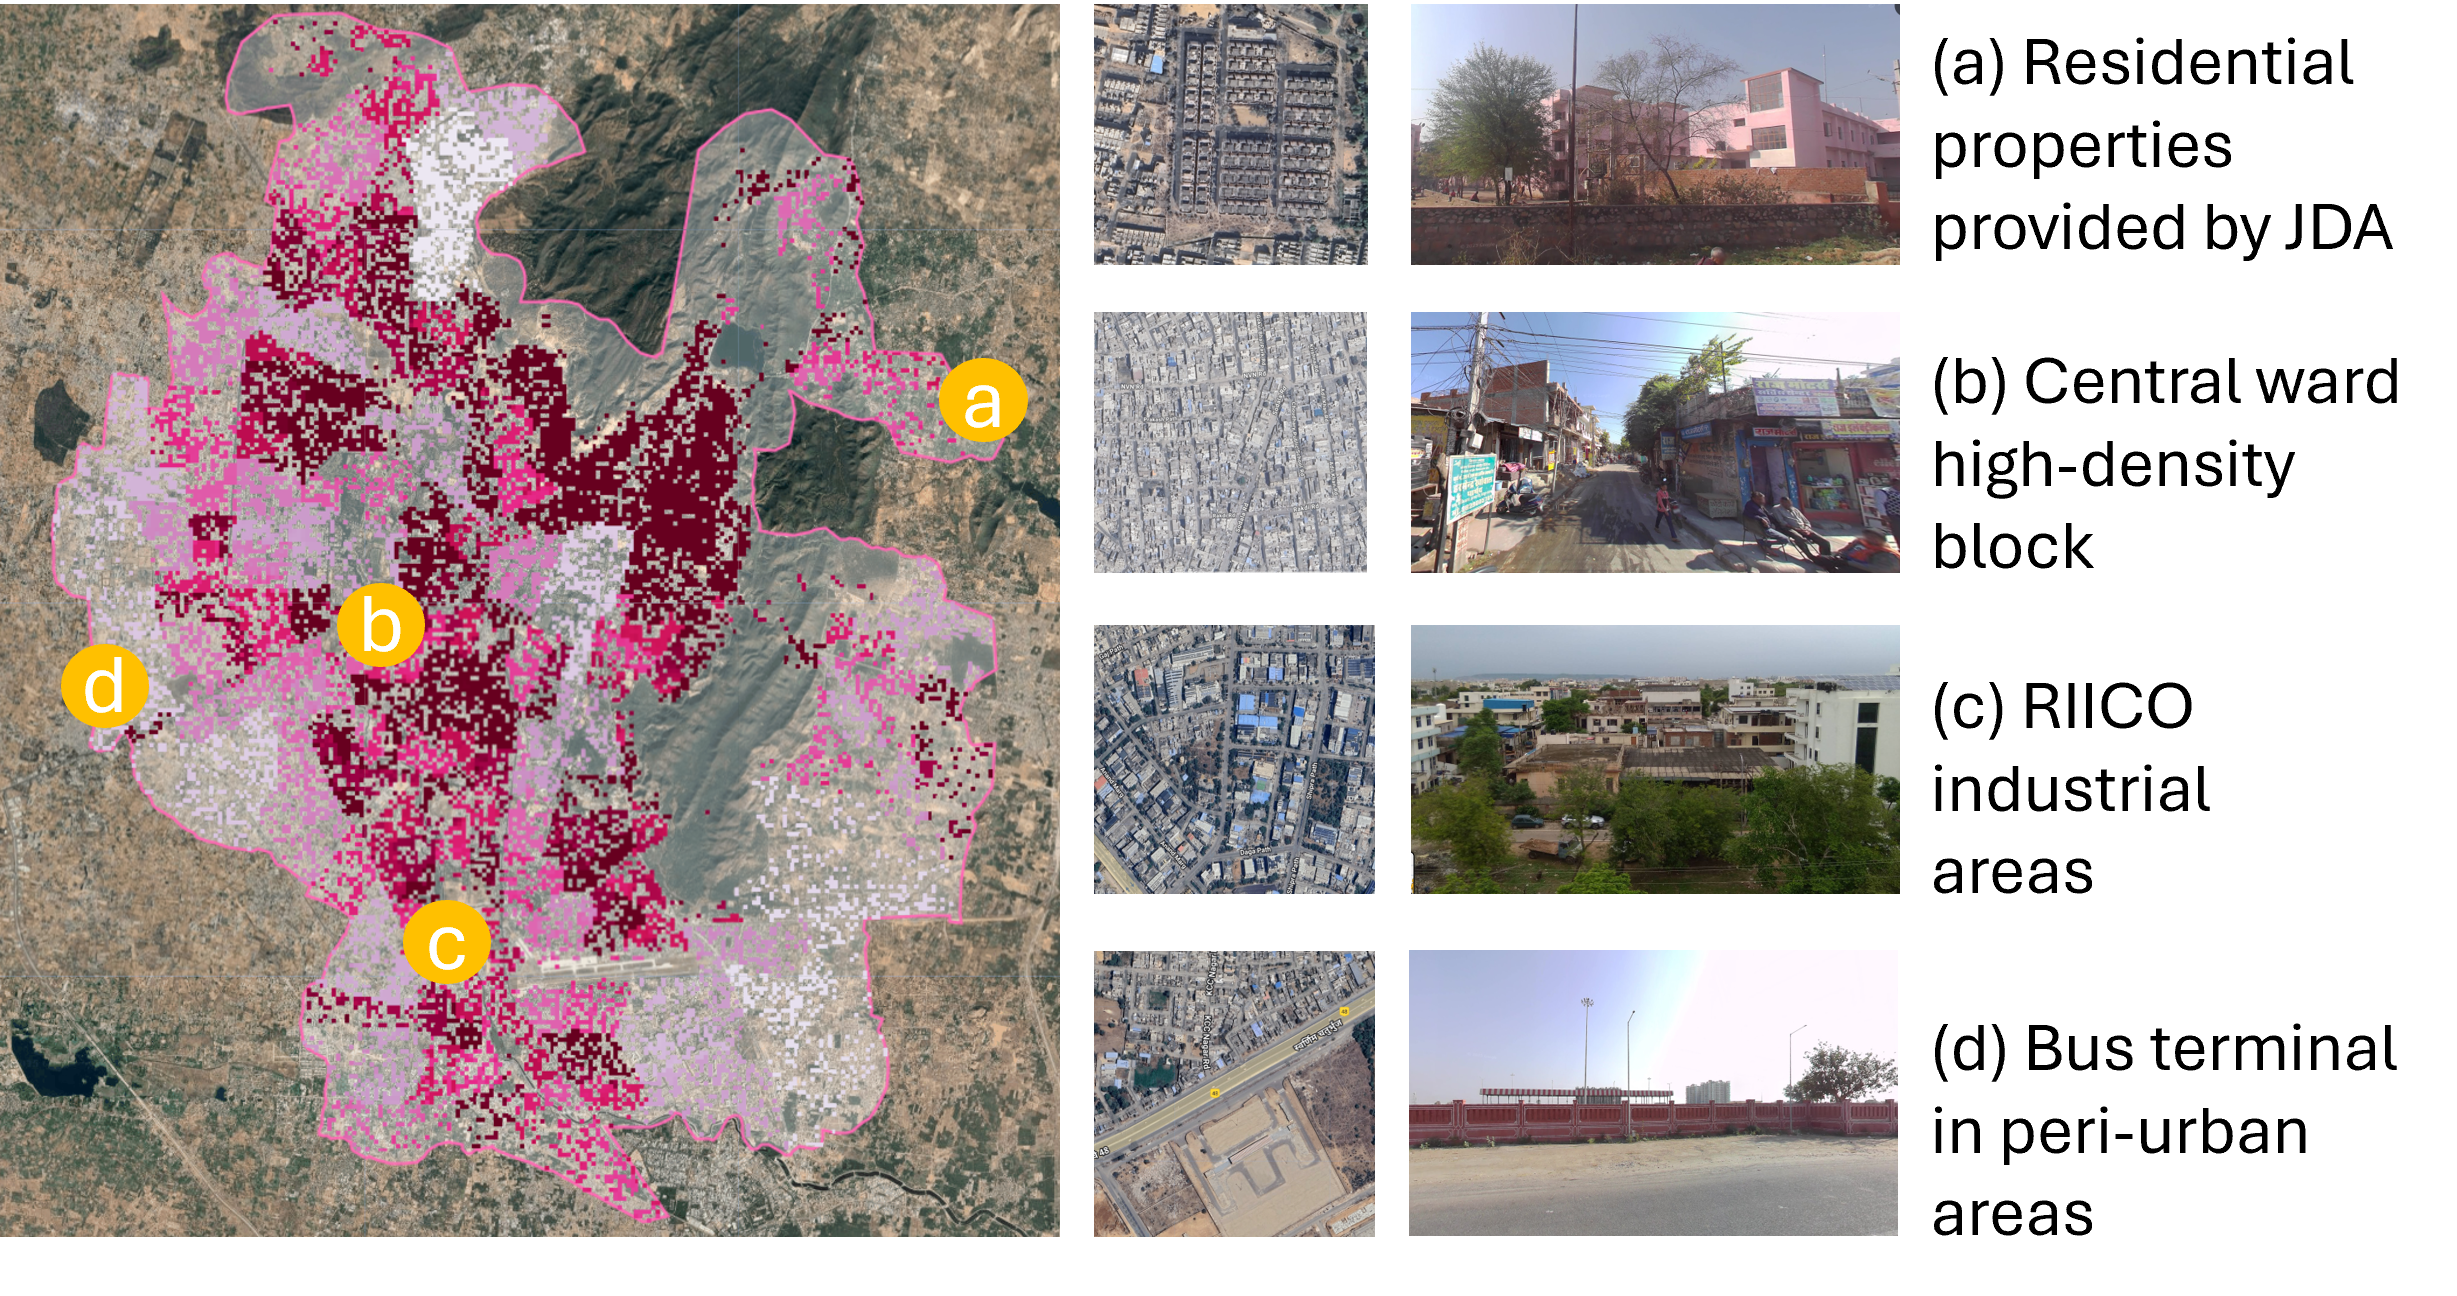
\includegraphics[width=0.96\linewidth]{thesis_images/05DI_8estimates_01} 

}

\caption{Spatial Distribution of four Population Overestimation Cases in Jaipur City (Basemap: Google).}\label{fig:05DI-8estimates-01}
\end{figure}

\begin{figure}

{\centering 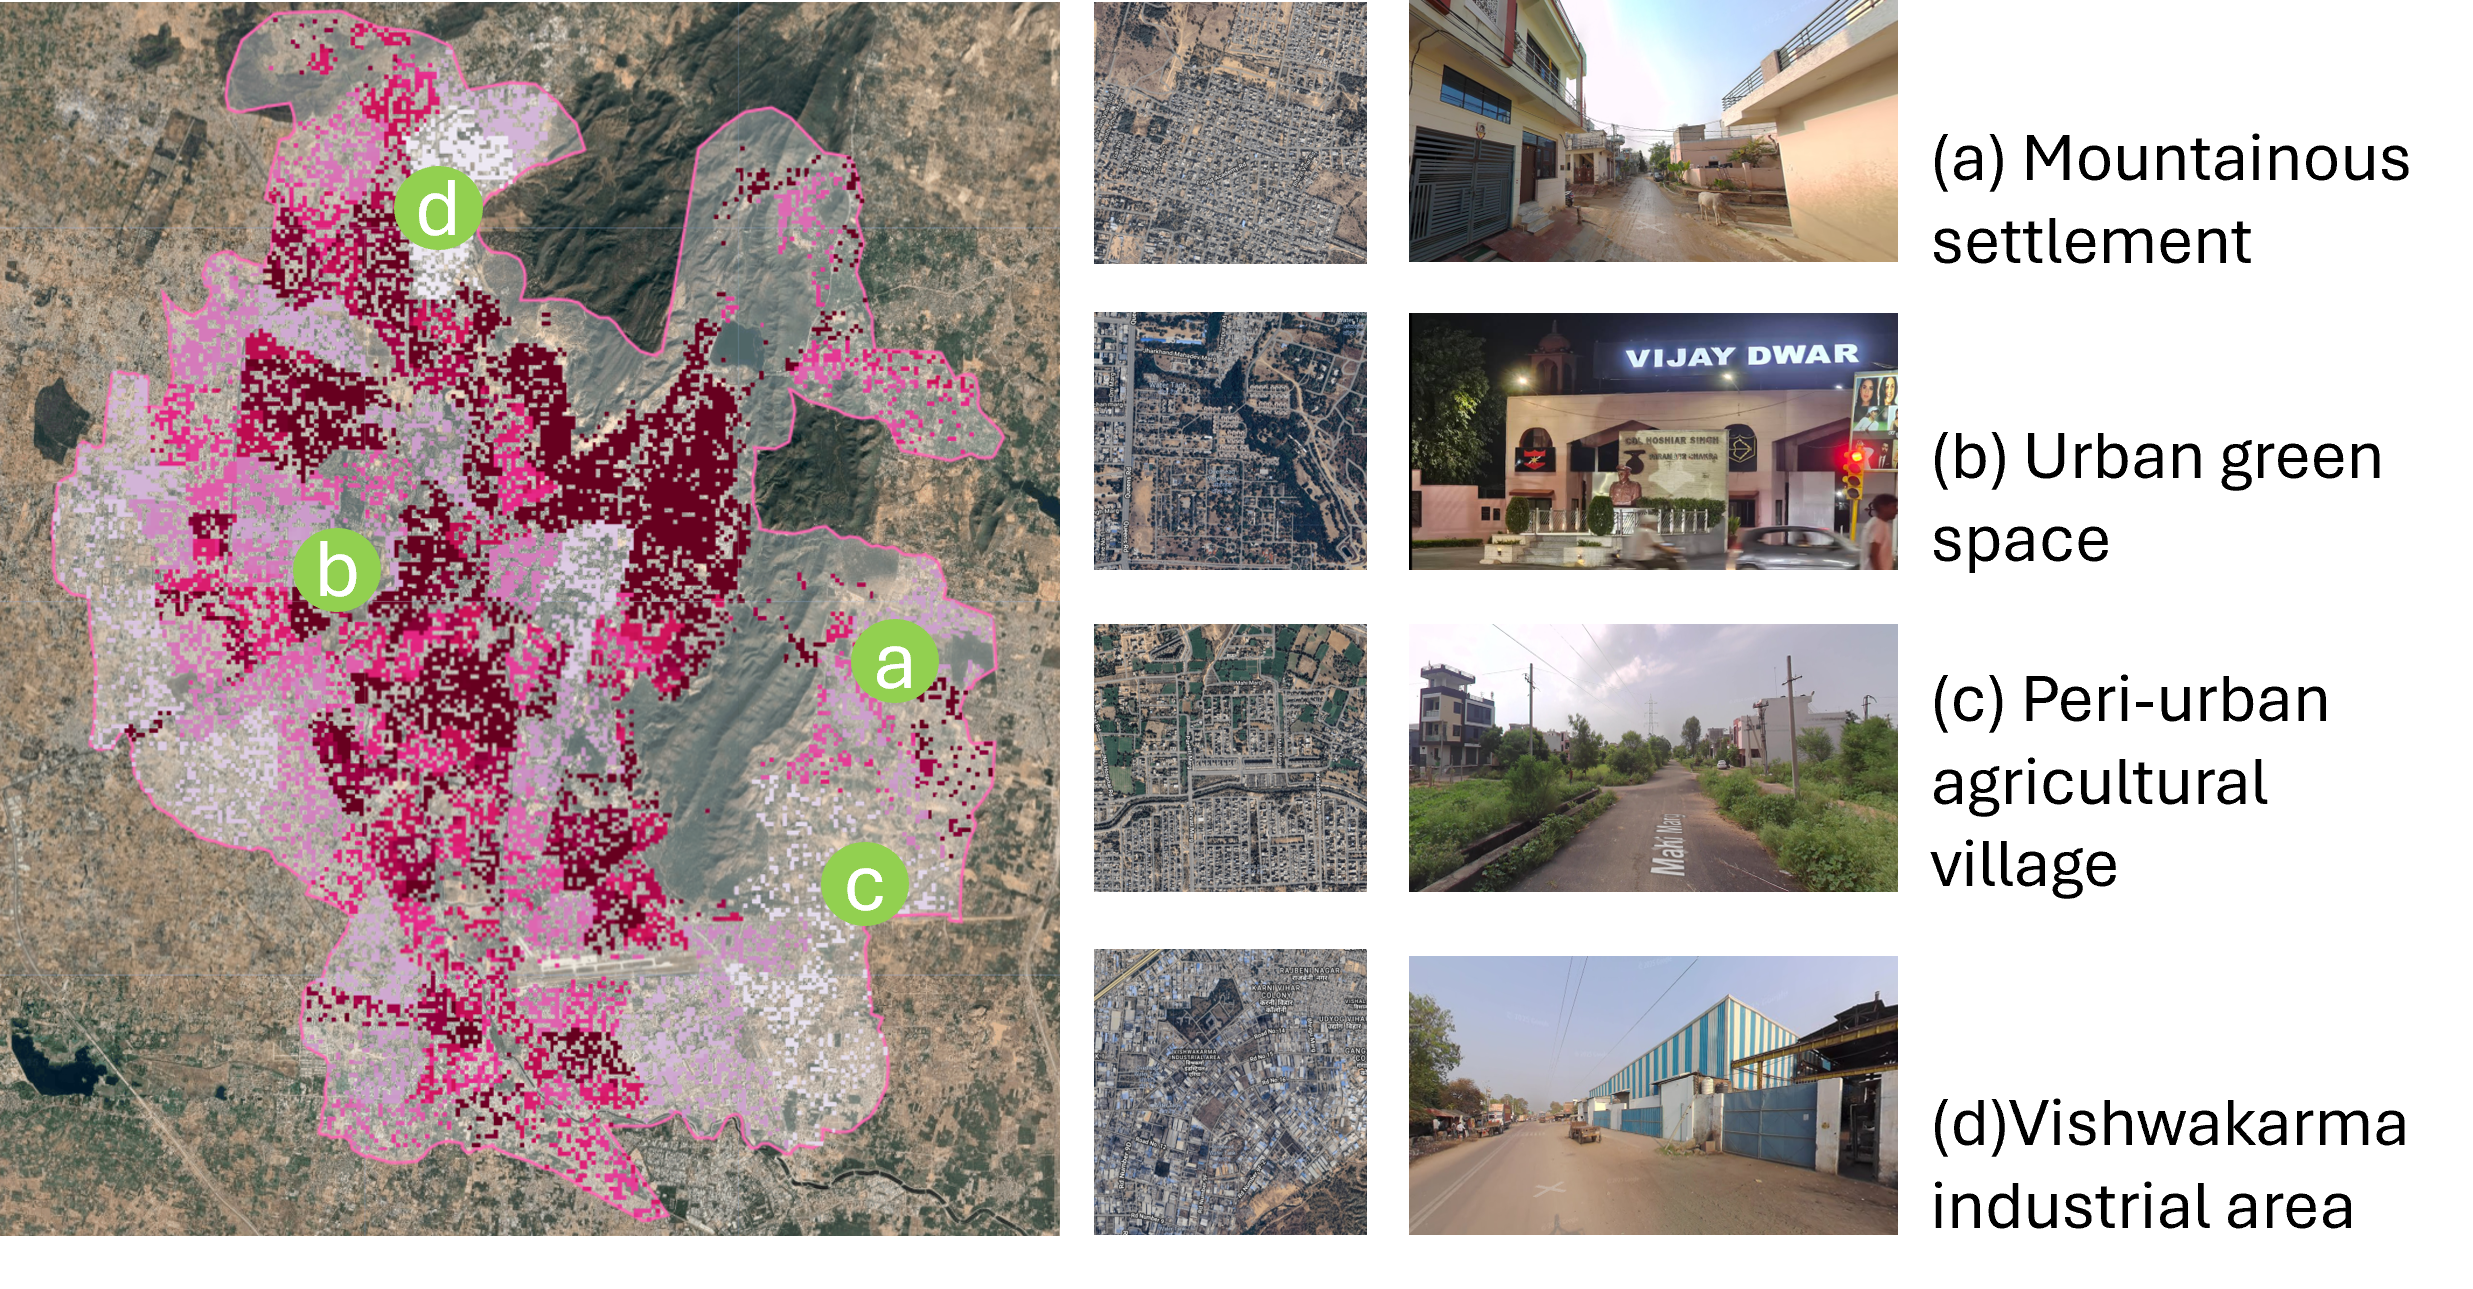
\includegraphics[width=0.96\linewidth]{thesis_images/05DI_8estimates_02} 

}

\caption{Spatial Distribution of four Population Underestimation Cases in Jaipur City (Basemap: Google).}\label{fig:05DI-8estimates-02}
\end{figure}

\section{Interpreting the EAI: Potentials and Methodological Limits}\label{interpreting-the-eai-potentials-and-methodological-limits}

The Economic Activity Index (EAI), derived from PCA, provides a compact representation of variation in Jaipur's economic environment. Its value lies not in the statistical process itself but in how it can be interpreted as a proxy for economic activity. One strength is its general alignment with the settlement structure. High values appeared in built-up corridors and dense residential areas, showing that variables such as built-up density, road density, POI density, population density, and nighttime lights captured major aspects of spatial intensity. Yet divergences also emerged. In the Vishwakarma industrial area, EAI values were high despite limited residential population, reflecting the influence of workplace POI and strong illumination. By contrast, some estates in RIICO industrial blocks showed high values both for population and for the EAI, pointing to the overlap between employment and nearby housing. These cases show that the EAI not only reflects population distribution, but also highlights workplaces and infrastructure that shape the urban economy.

At the same time, the PCA loadings raise interpretive challenges. A first issue is polarity. NDVI loaded negatively on PC1, which meant greener areas systematically reduced EAI values. This is statistically consistent because vegetation is often inversely related to built-up density. However, in planning practice, green space is usually seen as improving the attractiveness and competitiveness of a city, so the sign is opposite to standard expectations. A similar problem is that some variables that are central to urban economies, such as large transport infrastructure, received relatively low weights because their correlations with other variables were weaker. This illustrates the tension between PCA's simplification of data structure and the multidimensional nature of urban economic life.

A broader limitation concerns PCA's role as a weighting device. PCA assumes that all indicators are reflections of one hidden factor and can be treated as similar in meaning. But economic activity is not like this. It is formed by different elements---such as density, accessibility, and services---that are not the same and cannot replace each other. If PCA is applied mechanically, important dimensions may receive low weights simply because they do not co-vary strongly with others. This creates two risks. First, dimensions that are theoretically central, such as accessibility or service location, may be undervalued in the index. Second, the results have limited transferability. The weights are sample- and time-dependent, so the same variable may play very different roles across cities or over time. For example, in Jaipur, NDVI reduced the index because vegetation marks peripheral or low-density areas. In contrast, in other cities, green areas may be associated with high-value residential or commercial districts. Similarly, the role of POI may shift over time as services cluster or disperse. These contingencies make it challenging to interpret PCA-based indices consistently and weaken their robustness as general measures.

In summary, the EAI is best seen as a descriptive surface. It reveals spatial contrasts in Jaipur's economic environment and highlights zones where settlement and infrastructure overlap or diverge. However, polarity mismatches, the down-weighting of theoretically important variables, and the dependence of weights on context all point to the limits of PCA as a basis for generalisable measures.

\section{Evaluating the GEE Web App for Digital Planning}\label{evaluating-the-gee-web-app-for-digital-planning}

The GEE web app in this study served as a medium for delivering analytical results rather than as a modelling tool. Its use highlights both strengths and limits for digital planning. Outputs from the population disaggregation and the EAI were made available through the app, allowing planners, researchers, and potentially wider audiences to interact with the findings. Most of the data processing was undertaken in Python using the \emph{geemap} package, which integrated vector layers with large remote sensing datasets, while the app itself demonstrated how outputs can be translated into an accessible form. Compared with conventional Planning Support Systems (PSS), which often depend on proprietary software, specialist training, and localised data integration, the GEE-based interface benefits from cloud computing and globally available datasets, making it easier to share and update. Its strengths lie in accessibility and interactivity, though limitations remain: GEE's modelling functions are constrained for more complex processes, and concerns about data governance and security persist, as GEE is a commercial platform. \autocite{zhaoProgressTrendsApplication2021}.

The main contribution of the GEE environment is that it lowers technical barriers. Its code editor, documentation, and instant visualisation make it more approachable for planners with GIS backgrounds than traditional programming environments. This reduces reliance on external experts and allows practitioners to experiment directly with data rather than passively receiving outputs from opaque models. By lowering the entry threshold, GEE also opens opportunities for broader participation. Members of the public with an interest in urban issues can use the same tools to explore spatial data, test analyses, and contribute to debates on city futures. In this way, GEE functions not only as an analytical instrument but also as a participatory platform.

As \textcite{danielDigitalDisruptionPlanning2021} note, professional planners have often lagged in adopting digital tools, lacking the skills to interpret or build models independently. Platforms like GEE help bridge this gap by combining coding and geospatial analysis in a single environment. This allows planners to test, adapt, and visualise models in real time, making the platform more than a channel for sharing results. It can act as a bridge towards more active forms of digital planning practice. Looking ahead, GEE's capacity to integrate machine learning with remote sensing inputs points to possible predictive applications, supporting planners in monitoring and anticipating urban change. While such uses were not explored here, they suggest that cloud platforms could evolve into lightweight and flexible alternatives to traditional PSS, particularly in data-scarce contexts.

\section{Limitations and Transferability}\label{limitations-and-transferability}

At the data level, each proxy brings uncertainty. Nighttime lights are widely used for population/GDP, but their relationships are non-linear and non-uniform. In Jaipur, they correlate well with built-up density, yet saturation and temporal noise can reduce their reliability of population estimates in dense urban cores, while inhabited but poorly lit areas remain underestimated \autocite{wuBuildingVolumeAdjusted2023}. For economic activity, the sensitivity of lights to GDP varies across sectors and settlement types, so economic changes in services or agriculture may not be consistently reflected \autocite{bluhmWhatCanWe2022a}. Also, building volume improves representation of urban morphology, but it is still subject to footprint inaccuracies and height errors. Moreover, residential population density is used as a proxy to reflect economic activity, resulting in overlooking daytime and transient groups that strongly shape the urban economy.

At the methodological level, the models also have limits. MGWR reveals spatial heterogeneity but is bounded by the chosen covariates (e.g., tenure, migration, informal processes lie outside scope). PCA compresses multiple indicators but its polarity, sample dependence, and interpretive ambiguity weaken robustness as a stable metric.

Regarding transferability, the findings point to both potential and caution. Proxies that perform strongly in Jaipur---such as lights or built-up density---may be less reliable in cities with different infrastructures, economies, or morphologies. Even so, the overall framework has wider relevance for data-scarce contexts. By combining open remote sensing data with lightweight analytical models, it offers a replicable entry point for estimating urban activity. But local conditions must guide interpretation. Factors such as metropolitan scale, growth history, or ethnic composition will shape how results should be understood.

Possible improvements can also be noted. Integrating multiple sources of remote sensing, such as SAR for built-up detection, LiDAR for vertical structure, or higher-frequency composites of nighttime lights, would reduce dependence on any single proxy. Beyond residential indicators, incorporating dynamic datasets such as commuting flows, mobile phone records, or origin--destination surveys could add an ambient population perspective. Even if such data are only available at local scales, they can still strengthen planners' ability to interpret urban activity in data-scarce settings.

In sum, the proxies and models used here provide useful entry points for analysing urban activity, but their effectiveness is conditional on data quality and local context. These limitations underline the need for cautious interpretation and point to opportunities for methodological improvement in future research.

\chapter{Conclusion}\label{conclusion}

The central question of this study was: how can digital and open-access planning be supported in a data-scarce context? Using Jaipur, India, as a case study, it explored methods for estimating urban activities from open and remote sensing data, and for translating these outputs into forms usable by planners through a web-based platform. Two stages of analysis were developed: residential population was estimated at the grid level using MGWR-based disaggregation, and an Economic Activity Index (EAI) was constructed through PCA to integrate multiple spatial indicators. Both outputs were then deployed in a GEE app, allowing planners and researchers to interact with the results.

The grid-level population model reproduced Jaipur's overall settlement structure while also revealing systematic local biases. Overestimation was found in commercial cores, transport hubs, and planned estates, where intense POI signals and nighttime lights outweighed modest residential presence. Underestimation occurred in hillside villages, institutional complexes, and peri-urban croplands, where weak proxy values masked sustained habitation. These discrepancies show that while remote sensing proxies capture the overall distribution of settlement, they often misclassify specific contexts, particularly where residential and non-residential uses overlap.

The EAI was designed to approximate the city's economic environment by combining indicators of density, infrastructure, services, and illumination into a composite measure. It captured corridors of concentrated economic activity and highlighted industrial zones with strong workplace presence but limited residents. In this way, the index reflected contrasts between settlement and economic intensity, showing how open datasets such as nighttime lights, built-up area, and POI can be used to reveal patterns of economic activity in the absence of conventional statistics. Together, these two stages demonstrate how population and activity can be inferred from globally available data sources, offering planners alternative perspectives on urban structure and economy in contexts where surveys are irregular or absent.

A further contribution of this study lies in the delivery. The GEE web app enabled outputs to be explored without specialist software, offering both accessibility and transparency. For practitioners in resource-constrained settings, such platforms illustrate how open data and cloud computing can deliver planning insights that are reproducible and shareable across institutional and public audiences. More broadly, in the Global South, where statistical surveys are irregular and access to proprietary planning tools is limited, the combination of remote sensing proxies and online delivery represents a practical step toward more open and collaborative planning support.

Limitations must also be acknowledged. Each proxy introduces uncertainty: nighttime lights saturate in dense cores and underestimate poorly lit settlements, while building volume depends on footprint accuracy and height assignment. MGWR is bounded by the set of covariates available, and PCA compresses diverse dimensions into a single component that may not always align with theory. Proxies that performed well in Jaipur may also behave differently in cities with distinct infrastructures or economies, restricting transferability. Future work should integrate multi-source remote sensing (e.g.~SAR, LiDAR, higher-frequency lights) and incorporate dynamic datasets (e.g.~commuting flows, mobile-phone records) to capture ambient populations and improve robustness.

In conclusion, this study has shown that in data-scarce contexts, open and remote sensing data combined with accessible web delivery can generate meaningful planning insights into population and economic activity. While not substitutes for detailed surveys, the approaches developed here provide a replicable pathway for producing indicative surfaces that planners can use to guide dialogue, experimentation, and decision-making. The work contributes both methodologically, by demonstrating how urban activities can be estimated from open data, and practically, by showing how results can be delivered in forms that expand access to digital planning support.

\addcontentsline{toc}{chapter}{Bibliography}
\printbibliography

\chapter*{Appendix A Research log}\label{appendix-a-research-log}
\addcontentsline{toc}{chapter}{Appendix A Research log}

\addtocontents{toc}{\protect\setcounter{tocdepth}{0}}

\begin{longtable}[t]{>{\raggedright\arraybackslash}p{3cm}>{\raggedright\arraybackslash}p{10cm}}
\toprule
\textbf{Time} & \textbf{Things finished}\\
\midrule
\endfirsthead
\multicolumn{2}{@{}l}{\textit{(continued)}}\\
\toprule
\textbf{Time} & \textbf{Things finished}\\
\midrule
\endhead

\endfoot
\bottomrule
\endlastfoot
25th March 2025 & proposal first initialized\\
7th April 2025 & first meeting with Jens about ethics form and how to kick off the research\\
30th April 2025 & try to redefine the research question and prepare for staff meeting\\
2nd May 2025 & staff meeting and restrict research questions after meeting\\
26th May 2025 & literature review on new resaerch questions\\
\addlinespace
28th May 2025 & Jens meeting on dissertation outline\\
30th May 2025 & staff meeting for understanding data avalibility\\
11th June 2025 & Jens meeting on data problem, topic and method\\
4th July 2025 & staff meeting for ensuring data avalibility\\
18th July 2025 & Jens meeting for discussing final methodology\\
\addlinespace
23rd July 2025 & Jens meeting for discussing data processing\\
4th August 2025 & finish all analysis code\\
6th August 2025 & finish gee app\\
12th August 2025 & reviewed literature review draft\\
20th August 2025 & finish all and proofreading\\
\addlinespace
22nd August 2025 & final proofreading\\*
\end{longtable}

\chapter*{Appendix B POI Kernel Density Correlation Matrix in MGWR}\label{appendix-b-poi-kernel-density-correlation-matrix-in-mgwr}
\addcontentsline{toc}{chapter}{Appendix B POI Kernel Density Correlation Matrix in MGWR}

\begin{figure}

{\centering 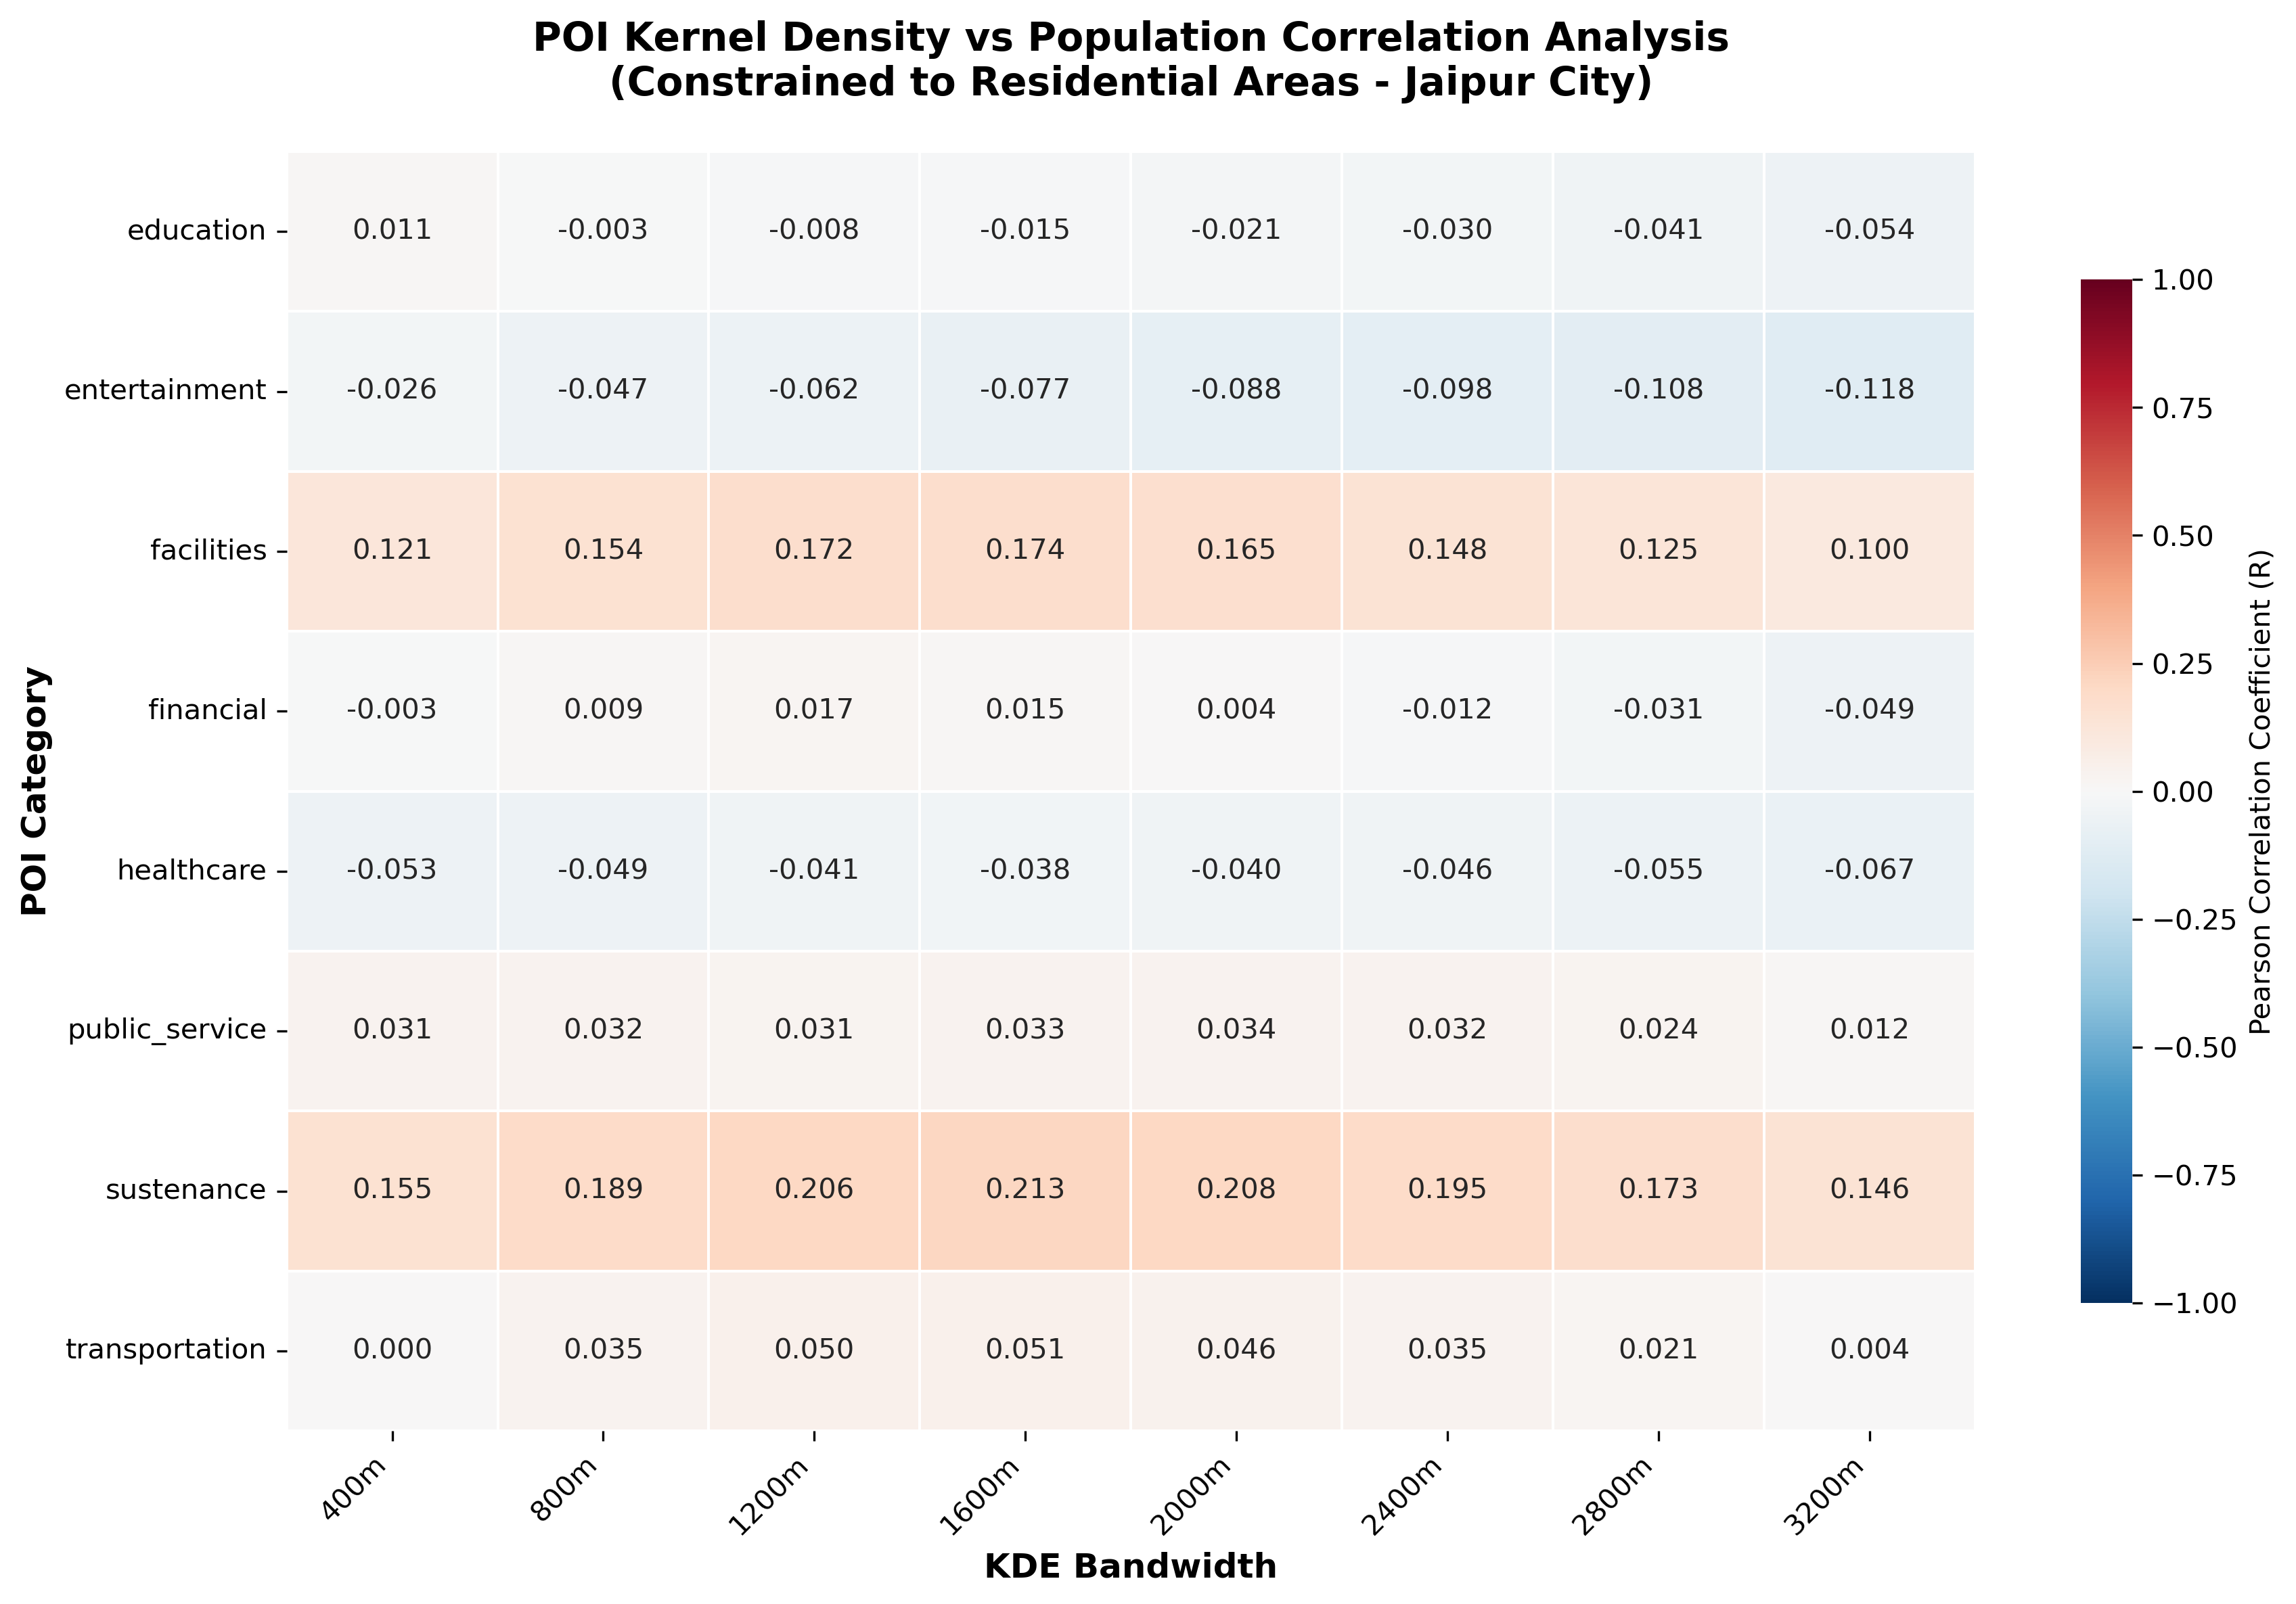
\includegraphics[width=0.9\linewidth]{thesis_images/Ab_jaipur_all_poi_correlation_heatmap} 

}

\caption{Heatmap of Pearson Correlations between POI Kernel Density and Ward Population Counts across KDE Bandwidths (Jaipur City, Residential Areas Only) }\label{fig:08Ab-mgwr-kde-matrix}
\end{figure}

\begin{figure}

{\centering 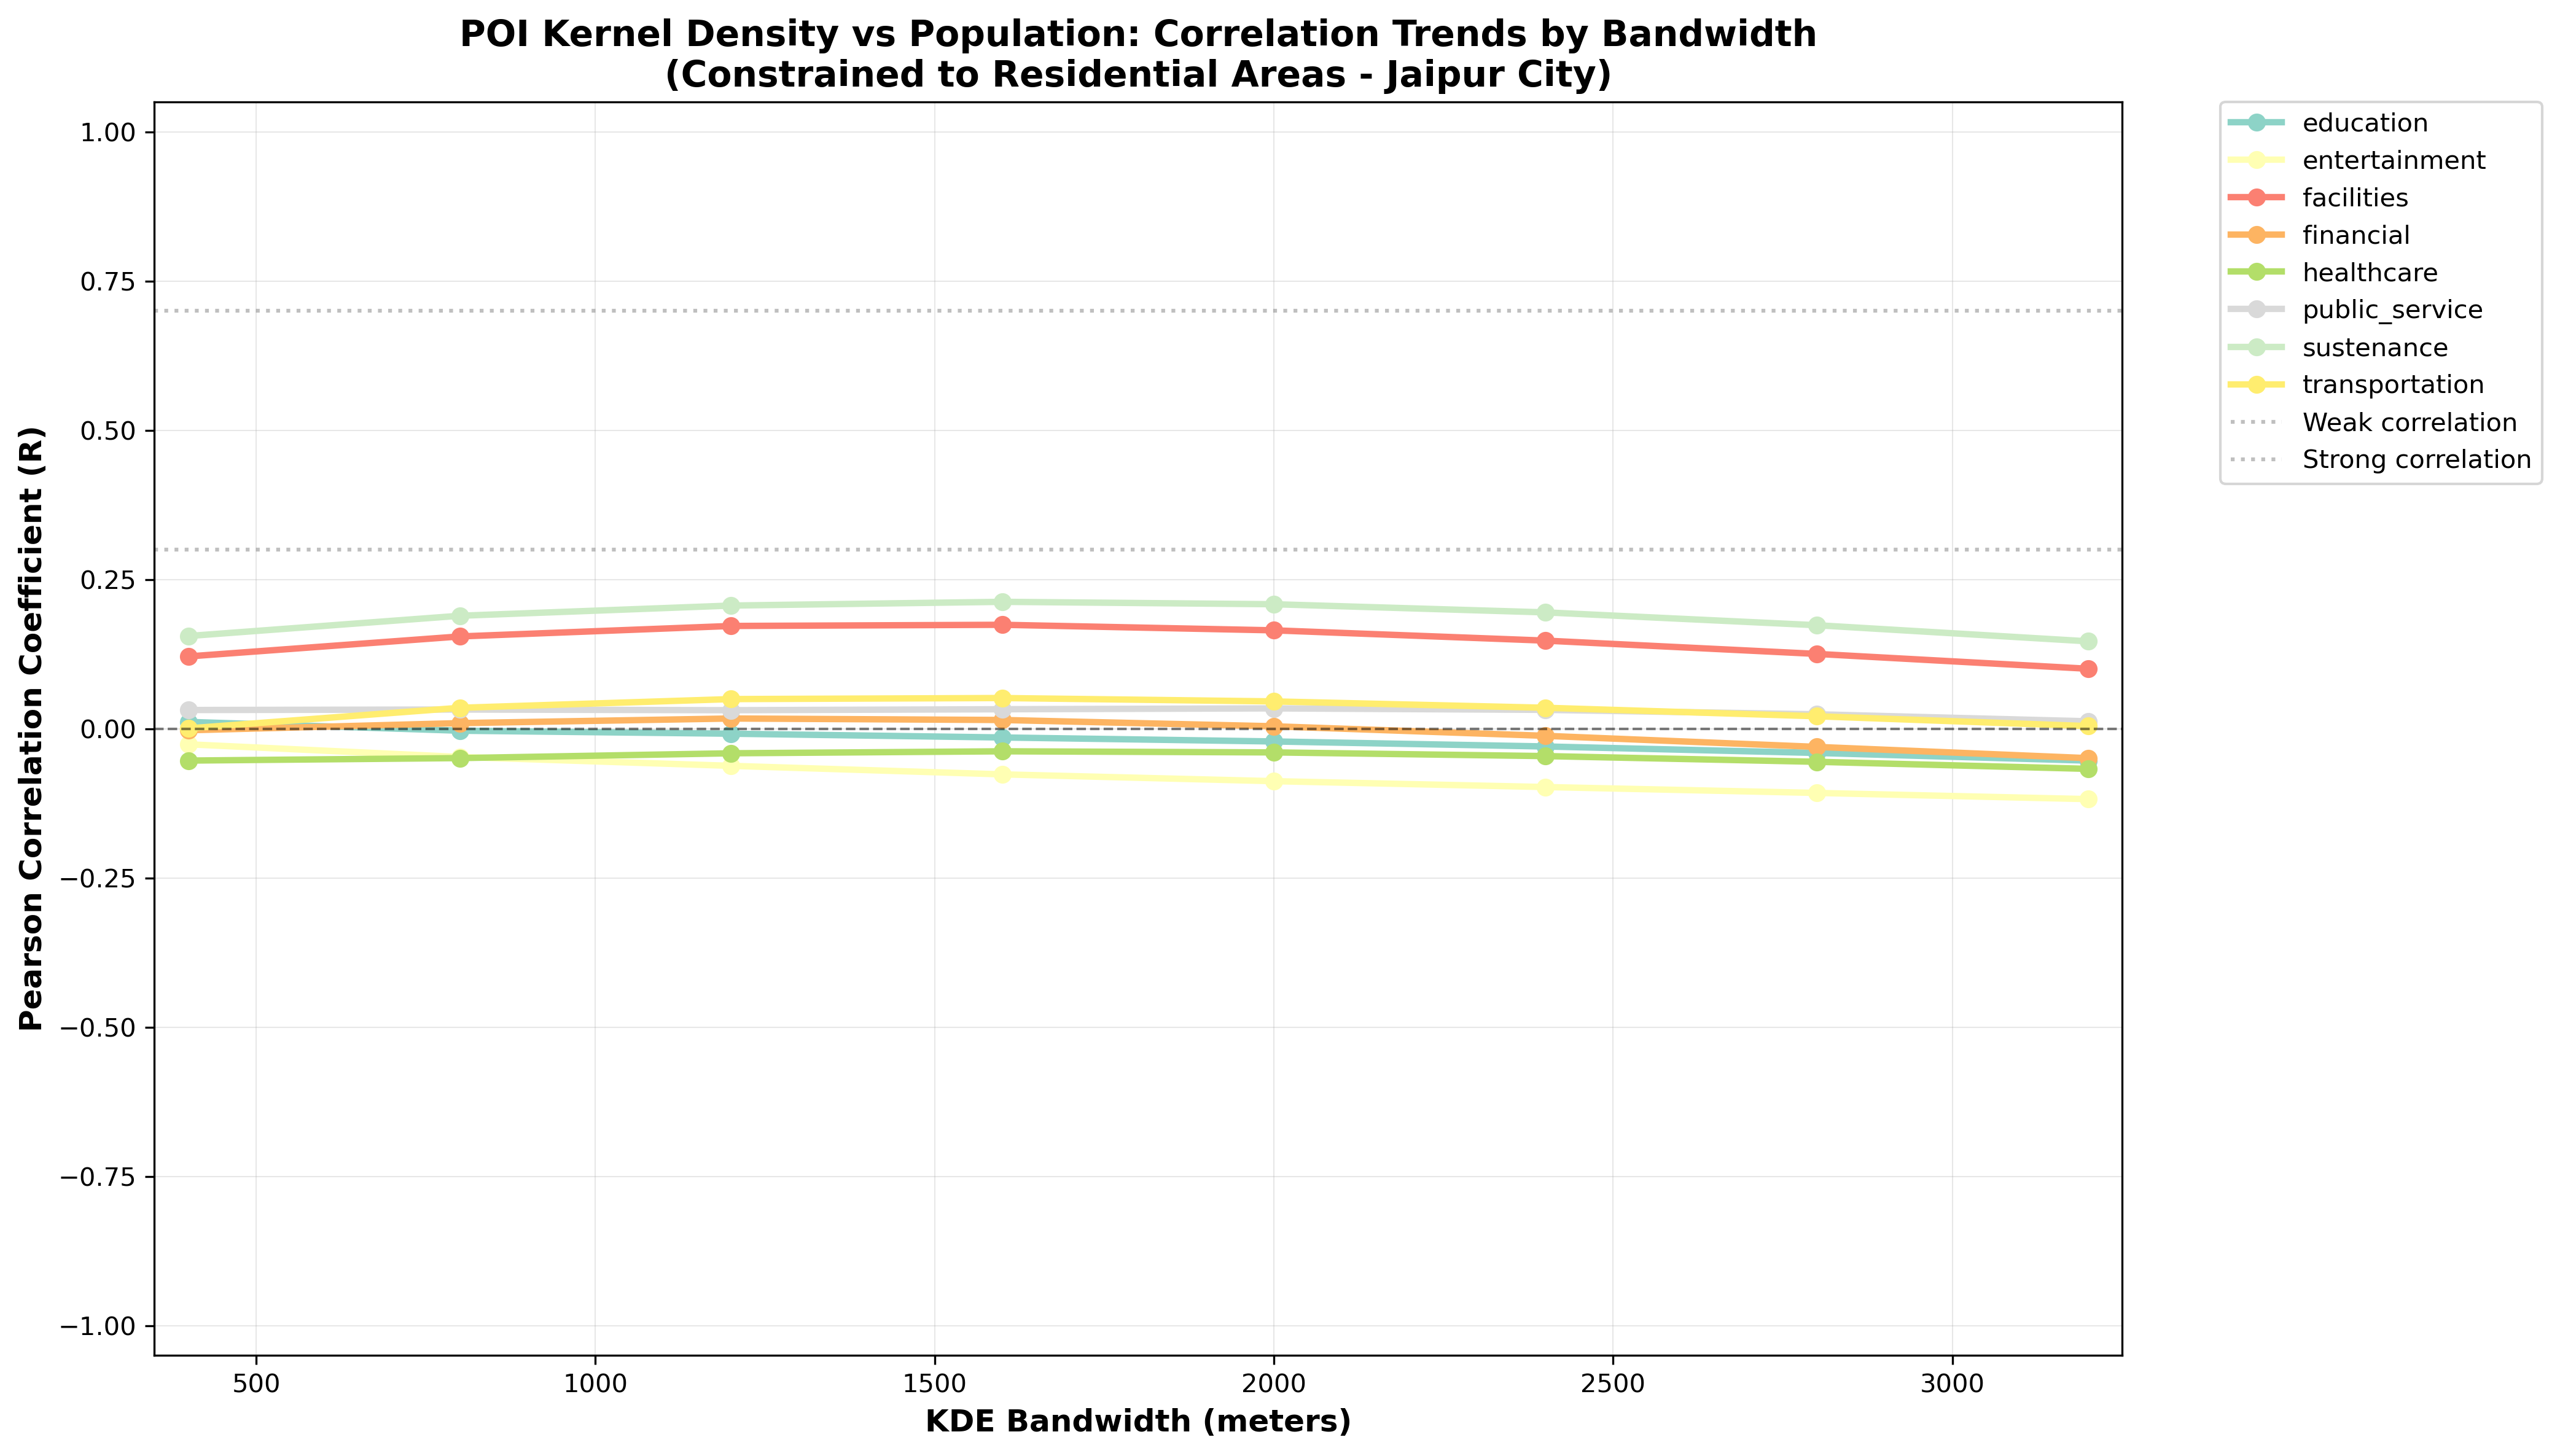
\includegraphics[width=0.9\linewidth]{thesis_images/Ab_jaipur_all_poi_correlation_trends} 

}

\caption{ Bandwidth-Sensitive Correlation Trends between POI Kernel Density and Ward Population Counts (Jaipur City, Residential Areas Only)}\label{fig:08Ab-mgwr-kde-pick}
\end{figure}

\chapter*{Appendix C Codes for Transformation Steps in MGWR Population Disaggregation}\label{appendix-c-codes-for-transformation-steps-in-mgwr-population-disaggregation}
\addcontentsline{toc}{chapter}{Appendix C Codes for Transformation Steps in MGWR Population Disaggregation}

\begin{Shaded}
\begin{Highlighting}[numbers=left,,]
\CommentTok{\# now this time this gpd is already have predictions of }
\CommentTok{\#logged grid{-}level population density}
\CommentTok{\# in df[Predicted\_log\_Y]}
\NormalTok{df }\OperatorTok{=}\NormalTok{ gpd.read\_file(}\StringTok{\textquotesingle{}data/cleaned/grid\_data\_for\_weights\_mgwr03.geojson\textquotesingle{}}\NormalTok{)}
\end{Highlighting}
\end{Shaded}

\begin{Shaded}
\begin{Highlighting}[numbers=left,,]
\CommentTok{\#{-}{-}{-} Step 2: Defining parameters and identifying areas {-}{-}{-}}

\CommentTok{\# Parameters for weighting}
\NormalTok{GAMMA }\OperatorTok{=} \FloatTok{0.5}  \CommentTok{\# Softmax sharpness: \textgreater{}1 sharper, \textless{}1 smoother}

\NormalTok{ALPHA }\OperatorTok{=} \FloatTok{0.5}  \CommentTok{\# Power transform for smoothing: \textless{}1 compresses high values}

\NormalTok{BASE\_WEIGHT\_UNINHABITED }\OperatorTok{=} \FloatTok{1e{-}9} \CommentTok{\# A very small base weight for }
\CommentTok{\#non{-}residential areas for visulisation, but does not }
\CommentTok{\#contribute to population as the remainder function }
\CommentTok{\#will not allocate any population to these areas.}

\NormalTok{WINSOR\_THRESHOLD }\OperatorTok{=} \FloatTok{0.99} \CommentTok{\# Percentile to cap extreme weights}

\CommentTok{\# Define inhabited vs. uninhabited areas based on a key variable}
\CommentTok{\# Using \textquotesingle{}illum\_vol\_density\textquotesingle{} is a robust choice.}
\NormalTok{uninhabited\_mask }\OperatorTok{=}\NormalTok{ (df[}\StringTok{\textquotesingle{}illum\_vol\_density\textquotesingle{}}\NormalTok{] }\OperatorTok{==} \DecValTok{0}\NormalTok{)}
\NormalTok{habited\_mask }\OperatorTok{=} \OperatorTok{\textasciitilde{}}\NormalTok{uninhabited\_mask}
\end{Highlighting}
\end{Shaded}

\begin{Shaded}
\begin{Highlighting}[numbers=left,,]
\CommentTok{\# Introduce a smoothing parameter epsilon in the Softmax function}
\CommentTok{\#{-}{-}{-} Step 3: Calculating preliminary weights (w\_pt) {-}{-}{-}}

\KeywordTok{def}\NormalTok{ softmax\_on\_scaled\_z(z\_vals, gamma}\OperatorTok{=}\FloatTok{1.0}\NormalTok{):}
    \CommentTok{"""Calculates softmax on min{-}max scaled values."""}
    \CommentTok{\# ensure working with a NumPy array}
\NormalTok{    z }\OperatorTok{=}\NormalTok{ np.asarray(z\_vals, dtype}\OperatorTok{=}\BuiltInTok{float}\NormalTok{)}
    \CommentTok{\# if all are nan, return an array of nans}
    \ControlFlowTok{if}\NormalTok{ np.isnan(z).}\BuiltInTok{all}\NormalTok{():}
        \ControlFlowTok{return}\NormalTok{ np.full\_like(z, np.nan)}
    \CommentTok{\# compute min and max ignoring nan}
\NormalTok{    z\_min }\OperatorTok{=}\NormalTok{ np.nanmin(z)}
\NormalTok{    z\_max }\OperatorTok{=}\NormalTok{ np.nanmax(z)}
    \CommentTok{\# if constant, return uniform weights}
    \ControlFlowTok{if}\NormalTok{ z\_max }\OperatorTok{==}\NormalTok{ z\_min:}
        \ControlFlowTok{return}\NormalTok{ np.full\_like(z, }\FloatTok{1.0} \OperatorTok{/}\NormalTok{ z.size)}
    \CommentTok{\# min–max scale}
\NormalTok{    z\_scaled }\OperatorTok{=}\NormalTok{ (z }\OperatorTok{{-}}\NormalTok{ z\_min) }\OperatorTok{/}\NormalTok{ (z\_max }\OperatorTok{{-}}\NormalTok{ z\_min)}
\NormalTok{    exps }\OperatorTok{=}\NormalTok{ np.exp(gamma }\OperatorTok{*}\NormalTok{ z\_scaled)}
    \ControlFlowTok{return}\NormalTok{ exps }\OperatorTok{/}\NormalTok{ np.nansum(exps)}

\CommentTok{\# a. Calculate softmax weights for HABITED areas}
\NormalTok{df[}\StringTok{\textquotesingle{}w\_raw\textquotesingle{}}\NormalTok{] }\OperatorTok{=}\NormalTok{ np.nan}
\NormalTok{df.loc[habited\_mask, }\StringTok{\textquotesingle{}w\_raw\textquotesingle{}}\NormalTok{] }\OperatorTok{=}\NormalTok{ df[habited\_mask].groupby(}\StringTok{\textquotesingle{}Id\textquotesingle{}}\NormalTok{)}
\NormalTok{[}\StringTok{\textquotesingle{}Predicted\_log\_Y\textquotesingle{}}\NormalTok{].transform(}
    \KeywordTok{lambda}\NormalTok{ z: softmax\_on\_scaled\_z(z.values, gamma}\OperatorTok{=}\NormalTok{GAMMA)}
\NormalTok{)}

\CommentTok{\# b. Apply alpha power transform to smooth the raw weights}
\NormalTok{df[}\StringTok{\textquotesingle{}w\_pt\textquotesingle{}}\NormalTok{] }\OperatorTok{=}\NormalTok{ np.nan}
\NormalTok{df.loc[habited\_mask, }\StringTok{\textquotesingle{}w\_pt\textquotesingle{}}\NormalTok{] }\OperatorTok{=}\NormalTok{ df.loc[habited\_mask, }\StringTok{\textquotesingle{}w\_raw\textquotesingle{}}\NormalTok{] }\OperatorTok{**}\NormalTok{ ALPHA}

\CommentTok{\# c. Assign a tiny base weight to UNINHABITED areas}
\NormalTok{df.loc[uninhabited\_mask, }\StringTok{\textquotesingle{}w\_pt\textquotesingle{}}\NormalTok{] }\OperatorTok{=}\NormalTok{ BASE\_WEIGHT\_UNINHABITED}
\end{Highlighting}
\end{Shaded}

\begin{Shaded}
\begin{Highlighting}[numbers=left,,]
\CommentTok{\#{-}{-} Step 4: Normalizing, winsorizing, and finalizing weights {-}{-}{-}}

\CommentTok{\# a. First normalization to get initial final weights}
\NormalTok{df[}\StringTok{\textquotesingle{}w\_initial\textquotesingle{}}\NormalTok{] }\OperatorTok{=}\NormalTok{ df.groupby(}\StringTok{\textquotesingle{}Id\textquotesingle{}}\NormalTok{)[}\StringTok{\textquotesingle{}w\_pt\textquotesingle{}}\NormalTok{].}
\NormalTok{transform(}\KeywordTok{lambda}\NormalTok{ w: w }\OperatorTok{/}\NormalTok{ w.}\BuiltInTok{sum}\NormalTok{())}

\CommentTok{\# b. Winsorize (trim) the weights to handle outliers}
\NormalTok{threshold }\OperatorTok{=}\NormalTok{ df[}\StringTok{\textquotesingle{}w\_initial\textquotesingle{}}\NormalTok{].quantile(WINSOR\_THRESHOLD)}
\NormalTok{df[}\StringTok{\textquotesingle{}w\_trim\textquotesingle{}}\NormalTok{] }\OperatorTok{=}\NormalTok{ np.minimum(df[}\StringTok{\textquotesingle{}w\_initial\textquotesingle{}}\NormalTok{], threshold)}

\CommentTok{\# c. Final re{-}normalization to get the final weights for disaggregation}
\NormalTok{df[}\StringTok{\textquotesingle{}w\_final\_trim\textquotesingle{}}\NormalTok{] }\OperatorTok{=}\NormalTok{ df.groupby(}\StringTok{\textquotesingle{}Id\textquotesingle{}}\NormalTok{)[}\StringTok{\textquotesingle{}w\_trim\textquotesingle{}}\NormalTok{].}
\NormalTok{transform(}\KeywordTok{lambda}\NormalTok{ w: w }\OperatorTok{/}\NormalTok{ w.}\BuiltInTok{sum}\NormalTok{())}
\end{Highlighting}
\end{Shaded}

\addtocontents{toc}{\protect\setcounter{tocdepth}{3}}
\enddocument

\printbibliography

\end{document}
